\documentclass[letterpaper, 12pt, oneside]{memoir}

\usepackage{GSAS} % uses GSAS style file we wrote

\begin{document}

\maxtocdepth{subsection} % put 4 levels into the toc

% Fill in title page
\settitle{Statistical and Machine \vspace{0.75ex} Learning Methods for Pattern \vspace{0.75ex} Identification in Environmental Mixtures} % your title
\setauthor{Elizabeth Atkeson Gibson} % your full name
\setinitial{Elizabeth A. Gibson} % your name with middle initial
\setyear{2021} % graduation/copyright year

% Here's the Title Page
\thetitlepage

% Here's the copyright page
\thecopyright

% Here's the Abstract
\thispagestyle{empty}
%\begin{GSASabstract}
\chapter*{Abstract}
\vspace{-2.5em}
\begin{center}
    \large \textbf{Statistical and Machine Learning Methods for Pattern Identification in Environmental Mixtures} \\
    Elizabeth Atkeson Gibson \\
\end{center}
\thispagestyle{empty}

Abstract of dissertation. In the abstract, you must (1) present the problem of the thesis/dissertation, (2) discuss the materials and methods used, and (3) state the conclusions reached. Individual chapters should not have abstracts.	Abstract of dissertation. In the abstract, you must (1) present the problem of the thesis/dissertation, (2) discuss the materials and methods used, and (3) state the conclusions reached. Individual chapters should not have abstracts.
	
\paragraph{Purpose of Review.}

The purpose of this review is to outline the main questions in environmental mixtures research and provide a non-technical explanation of novel or advanced methods to answer these questions.

\paragraph{Recent Findings.} 

Machine learning techniques are now being incorporated into high-dimensional mixture research to overcome issues with traditional methods. Though some methods perform well on specific tasks, no method consistently outperforms all others in complex mixture analyses, largely because different methods were developed to answer different research questions. We discuss four main questions in environmental mixtures research: 1) Are there specific exposure patterns in the study population? 2) Which are the toxic agents in the mixture? 3) Are mixture members acting synergistically? and 4) What is the overall effect of the mixture? 

\paragraph{Summary.} 

We emphasize the importance of robust methods and interpretable results over predictive accuracy. We encourage collaboration with computer scientists, data scientists, and biostatisticians in future mixtures methods development.

\thispagestyle{empty} 
\clearpage

%\end{GSASabstract}

\frontmatter % lowercase Roman page numbers for the next sections

\clearpage\tableofcontents
\clearpage\listoffigures
\clearpage\listoftables

% Abbreviations
\clearpage\chapter{List of Abbreviations}
\vspace{-3em}

% to start tables at top of page
\makeatletter
\setlength{\@fptop}{0pt}
\setlength{\@fpbot}{0pt plus 1fil}
\makeatother

\begingroup
\renewcommand{\arraystretch}{1.25}
\begin{table}[!ht]
\centering
\begin{tabular}{p{3cm}l}
24-DCP & 2,4-dichlorophenol  \\
25-DCP & 2,5- dichlorophenol \\
AIC & Akaike information criterion  \\
B-PB & Butyl paraben  \\
BIC & Bayesian information criterion \\
BKMR & Bayesian kernel machine regression  \\
\bnmf & Bayesian non-parametric non-negative matrix factorization  \\
BP-3 & Benzophenone-3 \\
BPA & Bisphenol A \\
BSID & Bayley Scales of Infant Development \\
BzBP & Benzylbutyl phthalate \\
CCCEH & Columbia Center for Children’s Environmental Health \\
CDC & U.S. Centers for Disease Control and Prevention  \\
CI & Confidence interval \\
CrI & Credible interval \\
DBP & Diastolic blood pressure \\
DEHP & Di(2-ethylhexyl) phthalate \\
DiBP & Di-isobutyl phthalate  \\
DnBP & Di-n-butyl phthalate \\
EDC & Endocrine disrupting chemical  \\
EPA & U.S. Environmental Protection Agency \\
\end{tabular}
\end{table}
\endgroup

\begingroup
\renewcommand{\arraystretch}{1.25}
\begin{table}[!ht]
\centering
\begin{tabular}{p{3cm}l}
HOME & Home Observation for Measurement of the Environment \\
IQ & Intelligence quotient \\
IQR & Inter-quartile range \\
Lasso & Least absolute shrinkage and selection operator \\
LOD & Limit of detection  \\
M-PB & Methyl paraben   \\
MBP & Mono-n-butyl   \\
MBZP & Mono-benzyl \\
MCAR & Missing completely at random \\
MCMC & Markov chain Monte Carlo \\
MCPP & Mono-3-carboxypropyl  \\
MECPP & Mono-2-ethyl-5-carboxypentyl \\
MEHHP & Mono-2-ethyl-5-hydroxyhexyl \\
MEHP & Mono-2-ethylhexyl \\
MEOHP & Mono-2-ethyl-5-oxohexyl  \\
MEP & Mono-ethyl \\
MIBP & Mono-isobutyl \\
MSE & Mean squared error  \\
\ncpcp & Non-convex square root principal component pursuit \\
NHANES & U.S. National Health and Nutrition Examination Surveys \\
NIEHS & U.S. National Institute of Environmental Health Sciences \\
NMF & Non-negative matrix factorization  \\
NMF-$\ell_2$ & Non-negative matrix factorization with squared error objective \\
NMF-P & Non-negative matrix factorization with divergence objective \\
NRC & U.S. National Research Council \\
NSF & U.S. National Science Foundation \\
NTP & U.S. National Toxicology Program \\
OLS & Ordinary least squares  \\
P-PB & Propyl paraben  \\
PCA & Principal component analysis  \\
PCB & Polychlorinated biphenyls  \\
PCP & Principal component pursuit  \\
\rootpcp & Square root principal component pursuit \\
\end{tabular}
\end{table}
\endgroup

\begingroup
\renewcommand{\arraystretch}{1.25}
\begin{table}[!ht]
\centering
\begin{tabular}{p{3cm}l}
PCP-LOD & Principal component pursuit with limit of detection penalty \\
PII & Personally identifiable information \\
PM & Particulate matter \\
PMF & Positive matrix factorization   \\
POP & Persistent organic pollutants   \\
SBP & Systolic blood pressure \\
SNMU & Sparse non-negative matrix underapproximation  \\
SVD & Singular value decomposition \\
sd & Standard deviation \\
TEF & Toxic equivalency factor \\
TEQ & Toxic equivalency score \\
WISC-IV & Wechsler Intelligence Scale for Children, 4th edition  \\
WQS & Weighted quantile sum regression \\
\end{tabular}
\end{table}
\endgroup

% end code to start tables at top of page
\clearpage
\makeatletter
\setlength{\@fptop}{0pt plus 1fil}
\setlength{\@fpbot}{0pt plus 1fil}
\makeatother

% Acknowledgements
\chapter{Acknowledgements}


% Dedication
\chapter{Dedication}

\mainmatter % begin Arabic numbers pages from here on

\chapter[Introduction]{Introduction: Complex mixtures, complex analyses, an emphasis on interpretable results}
\vspace{-3em}

\begin{center}
Elizabeth A. Gibson,\textsuperscript{1} 
Jeff Goldsmith,\textsuperscript{2} 
Marianthi-Anna Kioumourtzoglou\textsuperscript{1} \\

\textbf{Affiliations:} \\ 
1. Department of Environmental Health Sciences, Columbia University; \\ 
2. Department of Biostatistics, Columbia University. \\ 

\textbf{Published as:} \\
Gibson EA, Goldsmith J, Kioumourtzoglou M-A. Complex Mixtures, Complex Analyses: an Emphasis on Interpretable Results. \textit{Current Environmental Health Reports}. 2019 May 8:1-9.
\end{center}
\label{sec:intro}

\clearpage

%% main text
\section{Background}\label{sec:Intro}

We are exposed daily to numerous environmental pollutants. Only a small proportion of these has been assessed for toxicity, with most studies conducted in experimental settings and not necessarily involving humans \citep{grandjean06}. Furthermore, studies evaluating adverse health have traditionally conducted single-chemical analyses. This approach, however, does not represent reality; we are exposed to a mixture of chemicals at any given time, which can act synergistically or antagonistically. Furthermore, due to high correlations among many of these chemicals, we might detect associations between some of them and the outcome of interest due to their correlation with the actual ``bad actor(s),'' i.e. the actual toxic agent(s) in the mixture. Finally, testing a plethora of chemicals in single-pollutant models---i.e., multiple comparisons---dramatically increases the chances of spurious findings and, consequently, may increase disagreement across studies. For these reasons, the US Environmental Protection Agency, National Research Council (NRC), and National Institute of Environmental Health Sciences have all recognized the necessity to assess exposure to mixtures \citep{epaSP, nrc}.

Assessing exposures to mixtures, nonetheless, is especially challenging. First, the dimensionality of the data dramatically increases when one includes multiple chemicals in the statistical model. Many studies do not have the power to accommodate this need. Furthermore, high correlation among chemicals can lead to collinearity and subsequently inflated standard errors and unstable effect estimates. Two main issues stemming from current limitations in mixtures analyses have been identified: the need for (a) novel and robust statistical approaches to assess exposure to mixtures, and (b) appropriate use of available statistical methods in epidemiologic studies \citep{taylor16}.

Given the increasing need to incorporate complex high-dimensional data in environmental health studies, researchers have progressively turned towards machine learning methods. Adapting machine learning and data science methods can be especially advantageous, leading to more comprehensive studies of environmental exposure impacts on human health. Nonetheless, these methods were developed to serve a different purpose, mostly focusing on optimizing predictive accuracy, which is not necessarily well-aligned with Public and Environmental Health. Environmental health researchers, therefore, should be especially cautious when using such methods, and preferably should work with computer and data scientists, in collaboration with biostatisticians, to best adapt and extend machine learning methods for appropriate use in environmental health. 

The goal of this paper is not to give a comprehensive overview of all existing methods to analyze exposure to mixtures. Instead, we will discuss four types of scientific questions that are of interest in mixtures research. We will provide a conceptual description of analytic techniques appropriate to answer each question, along with examples in recent studies. No single method, to date, can adequately address all four types of mixtures-related scientific questions \citep{taylor16}. Although other reviews exist on mixtures methods \citep{hamra2018environmental, stafoggia2017statistical, huang2018cumulative, coker2018multi}, here we emphasize the need for methods that ensure robust results while focusing on interpretability and inference. Although the specific research question(s) might differ across studies, the two aims of mixtures analyses are universal: to (1) better understand biological pathways of pathogenesis, and (2) inform maximally efficient targeted interventions and policies to best protect the public and prevent disease. For both of these aims, it is of utmost importance to select {\textbf robust} methods that provide {\textbf interpretable}, and therefore actionable, results.

\section{Complex mixture methods}\label{sec:Methods}

Generally, exposure to a mixture indicates exposure to multiple ``stressors'' simultaneously, which can include both chemical and non-chemical (e.g., socioeconomic status, diet, etc.) components. The question becomes, how can we represent the complexity of reality in a statistical model? 

The selected method(s) should be based on the primary research question. If the interest lies in identifying exposure patterns or groups of people with similar exposure profiles, some dimensionality reduction is required \citep{jolliffe02, jolliffe02b, thompson04, paatero94}. To identify the toxic agent(s) in a mixture, variable selection approaches may be more appropriate \citep{tibshirani96, zou05}. If the aim is to evaluate synergistic or antagonistic effects, the main options are to hard-code interactions into the health model or take advantage of more flexible semi- or non-parametric models \citep{bobb2014bayesian,coull2015,bobb2018statistical}. Finally, to observe the effect of the overall mixture, one may create a weighted index of exposure or compute the full posterior distribution using Bayesian methods \citep{carrico15,bobb2014bayesian,coull2015}.

We present the four main research questions most relevant for mixtures analyses in Table~\ref{tab:qx}. In the next sections, we describe appropriate methods to address each of these questions and provide applied examples. Please note that many of the methods discussed may answer multiple questions and thus fall under multiple subsections. To avoid repetition, we present applications under the research question to which they contribute most uniquely. \\

\begin{table}[ht]
\begin{center}
\caption{The four main possible questions in mixtures analyses.}
\label{tab:qx}
\begin{tabular}{|c p{15cm}|}
\hline
  1. & Are there specific patterns of exposure in the study population? \\
  % \hline
  2. & Which are the toxic agents in the mixture? Or, what are the independent effects of each mixture member on the health outcome of interest? \\
  % \hline
  3. & Are there synergistic effects or interactions among mixture members? \\
  % \hline
  4. & What is the overall effect of the mixture on the outcome of interest? \\
\hline
\end{tabular}
\end{center}
\end{table}
\vspace{-2em}

\subsection{Pattern or profile identification}\label{sec:Patterns}

Identification of exposure patterns in the population, e.g. due to common sources or behaviors, is highly desirable if the goal is to inform targeted interventions and regulations. Once common patterns are identified, they can be included as the exposures of interest in health models, resulting in subsequent identification of the most toxic sources/behaviors. Regulatory agencies, then, can act on certain sources, and interventions can be designed to target specific behaviors. Methods adopted from the pattern recognition field are powerful tools to help researchers identify these shared exposure patterns. 

Questions about pattern or profile identification usually involve \textit{unsupervised} techniques to describe the variability among correlated chemicals in fewer unobserved (i.e., latent) factors or to identify subgroups of individuals with similar exposure profiles (i.e., clusters). The solution of unsupervised approaches is obtained independently of any outcome(s) of interest. Both clustering and factor analysis involve dimensionality reduction of the original data. Clustering groups study analysis units (e.g. participants in a cohort study or days in a time-series), and factor analysis techniques group chemicals into factors using combinations of the mixture members within each factor, i.e. patterns. To be meaningful, the number of clusters or patterns should be substantially lower in dimension than the original data. 

Clustering partitions observations (e.g., study participants) into distinct homogeneous groups so that observations within groups are similar and observations across groups are different. Clustering is often used in exploratory analyses, although the identified clusters can later be included in a health model as indicators. Though clustering is not particularly useful in estimating main effects, this approach can be advantageous when assessing effect modification by high-dimensional modifiers \citep{mak15_clusters}. Although the results from clustering can be quite interpretable, there is no ``golden rule'' for choosing the number of clusters \citep{ISLR}, highlighting the importance of expert knowledge in interpretation.

It may be more appropriate in environmental mixtures analyses to identify exposure patterns as functions of all mixture members representing specific sources of exposure or common behaviors in the study population. Pattern identification requires expert knowledge to assign interpretable labels to the estimated patterns. Principal component analysis (PCA) is the most commonly used dimension reduction technique employed in environmental epidemiology \citep{jolliffe02, pang16, mak14_unc, robinson2018urban, manzano2015tnf}. PCA aims to explain as much of the total variance in the data as possible using a smaller number of variables (called components), which are linear combinations of the original variables. The researcher must then decide the appropriate number of components to include in further analyses based on predefined criteria, by e.g. having {\textit a priori} defined a desired amount of the total variance explained. Although PCA is still widely used, its limitations include an orthogonal solution (which might be contrary to reality if the exposure patterns to be identified are not independent), no guarantee of an interpretable solution, and reliance on the researcher to decide on the number of components to retain for subsequent analyses.

While more advanced methods of matrix factorization exist \citep{candes11} including positive matrix factorization (PMF) and sparse non-negative matrix underapproximation (SNMU), the structure of the results appears largely similar. PMF and SNMU are similar to traditional factor analysis in that the number of mixture components is designated by the researcher \citep{gillis2010, gillis2013, paatero94}, but they both include constraints in the matrix factorization that enhance interpretability. First, the non-negativity constraint in both PMF and SNMU ensures that individual scores and variable loadings on factors are on the same range as the original variables \citep{lee2001, paatero94}, as all environmental data are positive (e.g. chemical concentrations). The factors and individual exposures can be easily described---factors by the relative proportions of variables, and individual exposures by the relative proportions of factors. Second, both PMF and SNMU, unlike PCA, provide non-orthogonal results which can more realistically describe human exposure \citep{paatero94, lee2001}. Finally, SNMU adds a sparsity constraint on the solution by including a penalty term forcing the lowest contributing variables in the factor loadings to zero, ignoring chemicals that do not add to the mixture \citep{gillis2013}.

Traor\'{e} et al. implemented SNMU to identify mixtures of 210 environmental contaminants, including pesticide residues, trace elements and minerals, in two cohorts of pregnant women in France \citep{traore2018}. The authors selected the optimal number of mixture components in terms of relevance and quality of interpretation, choosing eight \citep{traore2018}. They additionally applied hierarchical clustering to identify groups of women with similar co-exposure profiles \citep{traore2018}, clustering participants based on the patterns identified by the SNMU.

\subsection{Identification of toxic agents and independent effects}\label{sec:Ind}

When interested in the identification of specific toxic agents within a mixture and the characterization of their exposure-response curves, the method of choice should help us estimate the independent effects of each mixture member. Any analysis, therefore, should incorporate information on the outcome of interest (i.e., {\textit supervised} approaches).

Variable selection is one family of methods that may aid in identifying toxic agents by choosing a subset of relevant mixture members. The most traditional form is subset selection, including automated forward and backward selection and best subset selection \citep{ISLR}. While these are easy to implement, they can be unstable, as small changes in the data can greatly affect variable inclusion in the model, and the uncertainty in the variable selection portion is ignored \citep{shen2002adaptive, fan2001variable}, resulting in an increased type I error rate \citep{leamer1978specification, raftery1996approximate, draper1995assessment}.

To address flaws in subset selection, penalized regression techniques can be used; these out-perform ordinary least squares (OLS) in their predictive capacity. Notably, penalized regression methods perform better in highly correlated settings, finding a unique solution even when the number of chemicals is larger than the number of observations \citep{fan2006statistical}. These methods cannot, as no method can, determine causal agents in highly correlated mixtures, but they continue to predict well in these settings, where OLS would provide unstable effect estimates and inflated standard errors. 

By penalizing the magnitude of the coefficients, ``unimportant'' variables shrink toward zero, i.e., their estimated effects are restricted, allowing estimation of the coefficients that are more strongly associated with the outcome. This trades some bias in the estimated coefficients for lower variance and overall mean squared error (MSE) of the predicted outcome.

Multiple penalization forms exist. Ridge regression shrinks the sum of the squares of the coefficients, resulting in non-zero coefficients that are smaller than or equal to those that would have been obtained using OLS \citep{hoerl1970ridge}. Lasso (Least absolute shrinkage and selection operator) shrinks the sum of the absolute values of the coefficients, which pushes some coefficients to zero, yielding a sparse solution \citep{tibshirani96}. Elastic net includes both penalization terms \citep{zou05}.

The penalization term in each above-mentioned approach includes a tuning parameter ($\lambda$) between zero (making the model equivalent to OLS) and infinity (where all coefficients are shrunk towards zero) \citep{friedman2001elements, ISLR}. Usually, model fitting includes a training set and a validation set to choose $\lambda$, followed by a test set to estimate the true MSE of the model \citep{daume2012course}. In environmental epidemiology, a test set may not be necessary and is often unavailable, but some form of hold-out or cross-validation analysis to justify the choice of $\lambda$ is warranted.

Lasso is more commonly used than ridge regression recently because it produces a sparse solution. It has been shown to outperform other penalized methods when there is a small to moderate number of moderate-sized true effects, while ridge regression performs better when there is a large number of small true effects \citep{tibshirani96}. When mixture members are highly correlated, ridge and elastic net will push coefficients toward each other \citep{zou05, hoerl1970ridge}; lasso will keep one of the correlated variables in the model and push the others to zero \citep{tibshirani96}. If multiple toxic agents in correlated mixtures are hypothesized, elastic net may provide the best balance of sparsity and inclusion of correlated variables that best predict the health outcome.

The coefficients for the selected variables are not necessarily the same as those that would have been obtained from OLS including only that subset. It is even possible for corresponding coefficients in the two models to be in different directions \citep{tibshirani96}. A large drawback for use of these penalization methods in environmental health is the difficulty in obtaining valid inferences, as the coefficients are non-linear and non-differentiable \citep{tibshirani96}. To overcome this, many researchers have first fit a penalized regression (e.g. Lasso) and subsequently included the selected variables in an OLS model. This practice is not well justified for inference, as it underestimates standard errors by ignoring uncertainty in the variable selection step.

Nwanaji-Enwerem et al. used an adaptive lasso to select PM$_{2.5}$ constituents associated with DNA methylation age \citep{nwanaji2017associations}. This approach incorporates user-specified weights to penalize individual coefficients differently, so that constituents with larger effects are penalized less than those with smaller effects \citep{zou2006adaptive}. The mixture of interest in their analysis included five PM$_{2.5}$ constituents (organic and elemental carbon, sulfate, nitrate, and ammonium), that made up 89\% of the total PM$_{2.5}$ mass concentration. With covariates fixed in the model so that only constituents could be penalized, sulfate and ammonium remained in the model, positively predicting Horvath DNA methylation age \citep{nwanaji2017associations}.

\subsection{Interactions}\label{sec:Interact}

Identification of potentially synergistic effects among chemicals is essential if there is reason to believe that the combined health effect is greater (or less) than the sum of the independent effects. This is often hypothesized when studying chemicals that share stereo-chemical features or that target the same biological pathway. If regulatory action or interventions aim only to lower exposure to one chemical below a certain threshold, while this chemical works synergistically with another, then the necessary reduction will be underestimated among people exposed to both chemicals. Methods to assess interactions between chemicals can identify susceptible groups in those exposed to interacting chemicals simultaneously. Interactions can be hard-coded into models, including lasso and weighted quantile sum (WQS) regression (see Section~\ref{sec:Overall}). However, this practice requires {\textit a priori} deciding which interaction terms to include and can only accommodate a small number of all potential high-order and non-linear interactions. To address this limitation, semi- or non-parametric methods are preferred.

Non-parametric methods make no assumptions about the functional form of the association, instead using tuning parameters to estimate a curve as closely as possible to each point without overfitting \citep{ISLR}. Such approaches can more accurately fit nonlinear exposure-response relationships and allow for non-additive interactions among all mixture members without explicitly including them in the model. Semi-parametric methods combine the flexibility of non-parametric models with a parametric portion which is computationally easier to estimate \citep{friedman2001elements}, allowing for the adjustment of potential confounders. However, such approaches often require a larger sample size than is typically needed for a parametric approach, since they do not reduce the problem of estimating the functional form of the data to a few parameters \citep{ISLR}.

Bayesian kernel machine regression (BKMR) is a semi-parametric technique that models the exposure-response relationship as a non-parametric kernel function of the mixture members, adjusting for covariates parametrically \citep{bobb2014bayesian, coull2015,bobb2018statistical}. The Gaussian kernel is commonly used for flexibly capturing a wide range of underlying functional forms, including non-additive interactions, without specifying the shape of the individual exposure-response curves or the existence of interactions among mixture members \citep{bobb2014bayesian, liu2007semiparametric}. BKMR also assesses independent effects, allows for component-wise or hierarchical variable selection, and estimates the overall effect of a mixture \citep{bobb2014bayesian, coull2015, bobb2018statistical}, but we include it in this section due to its unique ability to detect nonlinear interactions.

Wasserman et al. used BKMR to estimate the joint effects of exposure to a mixture of five metals (arsenic, lead, manganese, cadmium, and selenium, measured cross-sectionally) and peri-natal arsenic on intellectual function in adolescents in Bangladesh \citep{wasserman2018cross}. While no interactions were observed, they found increased arsenic and cadmium were associated with decreased raw full scale IQ, as was the overall mixture exposure \citep{wasserman2018cross}.

Other methods to assess high-order and non-linear interactions include tree-based methods \citep{friedman2001elements}. Regression and classification decision trees yield highly interpretable results, but they tend to be unstable, i.e., small changes in the data can cause large changes in the estimated trees. More complex tree-based methods, such as random forests, are more robust to variation and have improved prediction, but they lose the interpretability of the single tree \citep{ISLR}. Several groups have begun to implement these methods in environmental mixtures \citep{stingone2017using, ouidir2017atmospheric, gass2014classification}.

\subsection{Overall mixture effect}\label{sec:Overall}

Characterizing the overall effect of combined chemical exposures is necessary to adequately define the total body burden of environmental mixtures. When exposure to individual compounds is below a set regulatory concentration or too low to show independent effects, an overall effect may still exist in combination with other exposures which target a common health endpoint. The NRC now recommends that risk assessment efforts account for cumulative risk associated with chemicals that affect the same health outcome \citep{national2009phthalates, huang2018cumulative}. If no interaction is present, i.e., effects are believed to be additive, a composite of chemicals or a weighted index allows for the estimation of the combined effects of individual compounds without reducing the unique exposures to a simple sum. 

Various methods exist to create a weighted score of exposure prior to the modeling step. Toxic equivalency factors (TEF), for example, are often used with dioxins and dioxin-like chemicals to weigh their toxicity in terms of the most toxic dioxin. Individual weights are determined by structural and binding similarities, ability to elicit a toxic response, persistence, and bio-magnification. A single number---a toxic equivalency (TEQ) score---is estimated as the sum of the products of each chemical's concentration and its individual TEF value, and can be used as a cumulative measure of exposure to these related chemicals \citep{van20062005, mitro2015cross}. Use of TEQ, however, is limited to chemicals whose main mechanism of action is shared with dioxin. Creating such indices, therefore, for other mixtures can be challenging, especially if such prior knowledge is not available.

When less is known \textit{a priori} about the individual toxicity of the mixture members, WQS regression creates an empirically weighted index which can be more widely implemented for any mixture. The estimated coefficient of this index is interpreted as the mixture effect \citep{carrico15}. As the name implies, WQS categorizes the continuous exposures into quantiles to reduce the impact of outliers and ensure that all exposure variables are on the same scale \citep{carrico15, gennings2013cohort}. but this also reduces the amount of information in the data. WQS is analogous to the variable selection methods discussed in Section~\ref{sec:Ind}, with each variable's penalization determined by its respective weight. WQS then assigns a single coefficient to the weighted index---the sum of the concentration quantiles of each member multiplied by its weight. The weights identify toxic agents and ``zero out'' chemicals with negligible associations \citep{carrico15, christensen2013multiple}. If the index coefficient is statistically significant, important components of the index (i.e., toxic agents) can be identified as those with the highest weights \citep{carrico15} The weights provide information on the relative importance of individual mixture members but no corresponding effect estimates. 

White et al. used WQS to estimate the overall effect of a mixture of ten metals (antimony, arsenic, cadmium, chromium, cobalt, lead, manganese, mercury, nickel, selenium) on breast cancer risk \citep{white2018metallic}. The WQS index was positively associated with postmenopausal breast cancer but not with overall or ER+ breast cancer. Cadmium, lead, and mercury had the largest weights in the postmenopausal breast cancer index \citep{white2018metallic}.

\section{Bayesian methods}\label{sec:Bayes}
Even though challenges still remain, recent advances in computational performance and scalability have opened the door to Bayesian methods in environmental epidemiology \citep{hoffman2013stochastic}. Bayesian methods explicitly use probability to quantify uncertainty in inference, i.e., there is (in principle) no impediment to fitting models with many parameters, correlated exposure variables, or complicated exposure-response specifications \citep{bda3}, and these methods may be used to answer multiple mixtures questions in the same analysis. Given the flexibility of Bayesian methods, they are a promising direction for new development.

Bayesian methods estimate the full posterior distribution of the unobserved quantities \citep{bda3}, meaning that all Bayesian models can estimate an overall effect. Additionally, inclusion of prior information---a hallmark of Bayesian data analysis---becomes a powerful tool in environmental mixture methods. Prior knowledge of effect estimates (magnitude or direction taken from expert knowledge or previous research) or chemical groupings (by exposure source, biological pathway, or shared toxicity) can be explicitly incorporated in the model.

BKMR, for example, assesses potentially non-linear independent effects and the overall effect in addition to interactions among mixture members. It also allows for hierarchical grouping of mixture members \citep{bobb2014bayesian, coull2015, bobb2018statistical}. Other examples of Bayesian methods in environmental mixtures exist, as well. Bayesian hierarchical methods \citep{maclehose2007bayesian, maclehose2014applications, furlong2017prenatal}, Bayesian model averaging \citep{fragoso2018bayesian, wilson2018model, berger2018associations, berger2018prenatal, berger2018associations2}, Bayesian additive regression trees \citep{park2014environmental, chipman2010bart, ko2016classification}, Bayesian profile regression \citep{coker2018multi, coker2017association, molitor2010bayesian}, and semi-Bayesian methods (which provide faster results) \citep{mak13_org,kalkbrenner2010perinatal,momoli2010analysis} have been implemented in environmental mixtures research, but they are not yet widely used. Computational advances in processing speed coupled with developments in machine learning and biostatistical modeling can make these methods accessible to environmental epidemiologists. There is space and need for more methods development, in collaboration with data and computer scientists and biostatisticians, in our field.

\section{Discussion}\label{sec:Discuss}

Although multiple methods currently exist for environmental mixtures research, no method can answer all mixtures questions, highlighting the importance of a well-defined research question to guide method selection. The interpretability of results (over predictive accuracy) is critical in determining the usefulness of novel statistical, data science, or machine learning methods in environmental epidemiology.

Despite statistical advances, all methods share certain limitations. Given high correlations across chemicals and varying measurement error in species-specific concentrations, any statistical method will pick the chemical with the least amount of measurement error that either is the toxic agent or is correlated with the toxic agent (but measured with less error) \citep{carroll2006measurement, pollack2012correlated}. Furthermore, if exposure biomarkers are used (e.g., chemicals or metabolites measured in biosamples), their half-lives and the timing of sample collection with respect to exposure matter. Depending on the chemical’s half-life and the critical window of exposure, all approaches are susceptible to selecting a chemical whose concentration was high during the critical exposure window and remained high during sampling; exposure to this selected chemical likely co-occurred with exposure to the actual toxic agent that---if it has a short half-life---might be undetected at sampling or measured with excess noise depending on the varying time between the critical exposure window and sampling across subjects. It is also conceivable that the actual toxic agent is not included in the mixture to be analyzed. Focusing, therefore, on identifying the toxic agent(s) might lead to the wrong conclusion under such scenarios, regardless of the choice (and performance) of method.

These issues may be amplified when the examined mixture is small, due to residual confounding from unmeasured chemicals or shared sources. Caution should also be applied when using the terms ``overall'' or ``cumulative'' for small mixtures, as these are usually only be a subset of the actual mixture of interest. The complexity of environmental mixtures---chemical and non-chemical---and analytical limitations for measurement of chemicals add to the difficulty of arriving at a perfectly-specified model. Including correlated exposure variables in any model may amplify rather than reduce confounding bias \citep{weisskopf2018bias}. Finally, uncertainty propagation is an often overlooked concern, mostly of unsupervised methods. Many researchers simply include PCA scores or cluster membership in health models ignoring the uncertainty inherent in the solution selection, often based on implicit assumptions. Propagation of uncertainty will lead to more valid inferences and can result in fewer spurious results and more consistent findings across methods and studies \citep{mak14_unc}.

In future mixtures analyses and methods development, researchers should focus on robustness of findings. Different populations experience different exposure mixtures and different distributions of potential modifiers, so we should not expect to replicate results (patterns or effect estimates) across populations. Rather, unstable methods should be avoided, and multiple methods should be used, whenever possible, to address a research question. When investigating an overall effect using WQS, for example, BKMR may be used as sensitivity analysis. Care should be taken, however, when employing different methods---if a specific research question is not stated, different methods may provide results that appear conflicting. For methods that employ simulations or rely on user-specified prior information (i.e., Bayesian methods), internal assessment of reproducibility is also warranted. 

These limitations and model-specific assumptions should be carefully considered when interpreting results of mixtures analyses. Additionally, groups developing mixtures methods should consider extensions that take this information into account when estimating health effects. Furthermore, combining methods may be of interest, for example coupling factor analysis with BKMR if one is interested in assessing the exposure-response of exposure patterns and their potentially non-linear interactions. 

Bayesian approaches, furthermore, inherently accommodate supervised pattern recognition, fully propagating uncertainty in the health model, thus identifying patterns specific to each outcome and better characterizing biological pathways. New Bayesian (and semi-Bayesian) methods could further allow more flexible modeling, explicit incorporation of uncertainty, inclusion of prior knowledge, and the ability to answer multiple questions simultaneously. Methods development should involve direct collaboration with computer scientists, data scientists, and biostatisticians to take advantage of computationally efficient machine learning algorithms and to obtain interpretable results from sophisticated models. Complex machine learning prediction methods generate enthusiasm across disciplines, but if their results are not directly interpretable in health effects analyses, they are unlikely to benefit the ultimate research goals of understanding biological pathways and informing regulatory action.

With careful incorporation of machine learning and data science methods, environmental epidemiologists are better able to explore complex relationships between environmental mixtures and adverse health. While each new prediction method appears to improve upon previous methods, effect estimation rather than outcome prediction should be the desired result. To this end, environmental epidemiologists must work with experts outside of our field to better adapt machine learning methods to our goals, instead of simply employing methods as they come. As methods development for environmental mixtures continues, we recommend Bayesian methods for their flexibility and interpretability of their results. Although no single model to date can answer all mixtures questions, a well-defined research question will point toward the correct approach---whether identification of patterns or independent, synergistic, or overall effect(s). Results are only useful, no matter how sophisticated the method, if they are robust, reproducible, interpretable and, finally, actionable.\footnotemark

\footnotetext{End of published work.}

\section{Dissertation overview}\label{sec:diss_over}

Environmental mixtures are an emerging topic in environmental health, and researchers agree that no single statistical or machine learning method can answer all potential questions in this area. The work presented in this dissertation focuses on a single mixture-related question: Are there specific patterns of chemical exposure in the study population? Because most dimensionality reduction methods employed in environmental epidemiology were not designed for this field, pattern recognition in  multi-pollutant exposure analysis contains several knowledge gaps. This dissertation details work to design, adapt, and apply statistical and machine learning methods to address environmental research questions.

In \textbf{Chapter~\ref{sec:ch2}} we introduce principal component pursuit (PCP), a robust dimensionality reduction method used in computer vision. PCP decomposes a chemical exposure matrix into a low rank matrix that captures consistent patterns in the data and a sparse matrix that isolates unique events \citep{pcp}. In this work, we adapted PCP to better accommodate environmental data. We included a non-negativity constraint on the low rank matrix and a novel penalty for values below the analytic limit of detection. We altered the algorithm to allow for missing values, and we specified a cross-validation procedure to choose the optimal rank of the low rank matrix. We compared PCP and PCA performance on simulated data, and we used PCP to separate consistent patterns from unique events in a mixture of persistent organic pollutants (POP) measured in the 2001--2002 National Health and Nutrition Examination Surveys (NHANES).

In \textbf{Chapter~\ref{sec:ch3}} we introduce Bayesian non-parametric non-negative matrix factorization (\bnmfc), adapted from work in the geological sciences built on previous NMF modeling techniques in machine learning \citep{holtzman2018machine, lee1999learning, cemgil2008bayesian, paisley2014bayesian}. \bnmf includes several features well-suited to environmental data. \bnmf generates all estimated values from Gamma distributions, which contain only non-negative real numbers ($\mathbb R_{\geq 0}^+$), and a non-parametric prior on the number of patterns chooses the optimal number from the data. We extended \bnmf by explicitly modeling the uncertainty in pattern identification. In \textbf{Chapter~\ref{sec:ch4}} we incorporated this uncertainty quantification into a novel hierarchical health model. 

The work presented in this dissertation aims to contribute to the development of robust methods to identify patterns of exposure in chemical mixtures. We addressed several key gaps in environmental mixture research. (1) The true number of patterns in a mixture is never known, and common methods employed by environmental health researchers require specification or selection of the correct number by the researcher. (2) Chemical concentrations are non-negative, and methods that return solutions containing negative values discard this information, making the solution less interpretable. (3) To our knowledge, no methods used for pattern identification in environmental mixtures quantify the uncertainty in this step; nevertheless, it is  often the first step of a two-stage process to estimate associations between identified patterns and health outcomes. With this work, we present two novel methods for pattern identification and aim to contribute to a better understanding of environmental mixture research and the type of questions that these tools can answer.

\clearpage

\chapter[Principal component pursuit]{Principal component pursuit for pattern identification in environmental health}\label{sec:ch2}
\vspace{-3em}
\begin{center}
Elizabeth A. Gibson,\textsuperscript{1} 
Junhui Zhang,\textsuperscript{2} 
Jingkai Yan,\textsuperscript{2}
Lawrence Chillrud,\textsuperscript{1} 
Jaime Benavides,\textsuperscript{1} 
Robert Colgan,\textsuperscript{2} 
Yanelli Nunez,\textsuperscript{1} 
Rachel Tao,\textsuperscript{3} 
Jeff Goldsmith,\textsuperscript{4} 
John Wright,\textsuperscript{2} 
Julie B. Herbstman,\textsuperscript{1} 
Marianthi-Anna Kioumourtzoglou\textsuperscript{1} \\ 

\textbf{Affiliations:} \\ 
1. Department of Environmental Health Sciences, Columbia University; \\ 
2. Department of Electrical Engineering, Columbia University; \\ 
3. Department of Epidemiology, Columbia University; \\
4. Department of Biostatistics, Columbia University. \\ 
\end{center}

\clearpage

%% main text
\chapter[Bayesian non-parametric non-negative matrix factorization]{Bayesian non-parametric non-negative matrix factorization for pattern identification in environmental mixtures}\label{sec:ch3}
\vspace{-3em}

\begin{center}
Elizabeth A. Gibson,\textsuperscript{1} 
Sebastian Rowland,\textsuperscript{1}
Jeff Goldsmith,\textsuperscript{2} 
John Paisley,\textsuperscript{3} 
Julie B. Herbstman,\textsuperscript{1} 
Marianthi-Anna Kioumourtzoglou\textsuperscript{1} \\

\textbf{Affiliations:} \\ 1. Department of Environmental Health Sciences, Columbia University; \\ 2. Department of Biostatistics, Columbia University; \\ 3. Department of Electrical Engineering, Columbia University. 
\end{center}

\clearpage

%% main text
\section{Introduction}
\label{intro}
Individuals are ubiquitously exposed to multiple classes of chemicals through environmental pollution and consumer products. Despite evidence from bio-monitoring studies indicating that exposures are often highly-correlated \cite{woodruff2011env}, environmental health research has historically examined single chemicals and classes in isolation. The combination of exposures, however, likely exhibits different relationships with potential health outcomes \cite{braun2016can, taylor16}. In recent years, there have been concerns regarding the health effects of environmental mixtures such as air pollution \cite{mak13_org}, heavy metals and metalloids \cite{wasserman2018cross}, and endocrine disrupting chemicals (EDCs) \cite{tanner2020early}. Due to common environmental sources or behaviors leading to exposure, potentially shared biological pathways, and similar toxicological effects, environmental health researchers often desire a tool for exposure pattern recognition \cite{gibson2019complex}.

To identify patterns in high-dimensional mixtures, researchers must overcome several challenges. First, the true number of patterns in a given population is not known. Existing methods employed in environmental health research use \textit{a priori} criteria specification (e.g., percent of variance explained by components in principal component analysis (PCA) or lowest Akaike information criterion (AIC) for Non-negative Matrix Factorization (NMF)) to choose the number of components retained or factors selected. This practice does not foster reproducibility of analyses, as two researchers using the same method on the same dataset may choose different criteria and, thus, obtain different results. Second, chemical concentrations are non-negative and, therefore, cannot be intuitively understood as a negative feature. Methods that return orthogonal solutions, such as PCA, and/or solutions that contain negative values (e.g., PCA, factor analysis, and various matrix factorizations) essentially discard this information, making the solution less interpretable. Potentially negative chemical loadings cannot be easily interpreted as either present or absent, and potentially negative individual scores do not intuitively convey exposure level. Third, pattern recognition in environmental health is likely the first step of a two-stage approach to estimate associations between identified patterns and health outcomes. This makes the estimation of uncertainty in the pattern recognition step essential for subsequent construction of appropriate confidence intervals of health effect estimates. Common methods such as PCA, NMF, and factor analysis do not quantify uncertainty in estimation.

In this paper, we introduce Bayesian non-parametric non-negative matrix factorization (\bnmfc) as an approach for identifying patterns in environmental mixtures. \bnmf decomposes observed exposure data (e.g., chemicals across participants in a cohort study or across days in a time series) into a matrix of chemical loadings and a matrix of individual scores on \bnmfc-identified patterns that are much smaller in number than the total number of chemicals. Because non-negativity is an informative feature of environmental exposure data, we enforced it on pattern loadings and individual scores with strictly non-negative priors, making them interpretable on an additive scale with a parts-based representation \cite{lee1999learning}.

Previous work on NMF comes from machine learning. \citet{lee1999learning} first introduced NMF as a method to learn a parts-based representation of data. In text analysis, NMF methods have been primarily applied to identify semantic features, or topics, of words shared across documents \cite{blei2003latent, paisley2014bayesian}. In the context of image recognition and compression, NMF methods have been applied to learn factors that correspond to parts of an original image and to reconstruct images that have been corrupted \cite{sandler2011nonnegative, cemgil2008bayesian}. Within environmental health, the majority of research employing pattern recognition methods has been in air pollution source apportionment, such as the U.S. Environmental Protection Agency's positive matrix factorization (PMF) \cite{paatero94}. The majority of NMF algorithms require the number of factors to be specified by the user. \bnmf stems directly from \citeauthor{holtzman2018machine}' implementation of a Bayesian non-parametric matrix factorization model to determine a suitable rank of factorization from the data. In their work, they employed NMF to identify frequency regions that co-occur across spectrograms to better identify changes in faulting processes leading to earthquakes \cite{holtzman2018machine}.

Our work provides several contributions to existing environmental exposure pattern recognition approaches. To our knowledge, this is the first Bayesian unsupervised statistical method considered for pattern recognition in mixtures of environmental exposures. Previous work in this area has utilized frequentist statistical and machine learning approaches in which the number of patterns in the mixture was specified by the researcher or treated as a tuning parameter. Here, we employed an empirical sparse prior on the number of patterns in the mixture to estimate it from the data. Additionally, we derived variational confidence intervals surrounding individual scores that provide previously unattainable uncertainty quantification. We conducted simulation studies (Section \ref{methods_sim}) in which we compared our method to other pattern identification methods, namely PCA, factor analysis, and two frequentist NMF models with different objective functions. Finally, we applied \bnmf to an environmental mixture of potential EDCs measured in pregnant women in a mother and child cohort from New York City (Section \ref{results_app}). This application highlights \bnmfc's ability to identify the number of underlying patterns in a chemical mixture without guidance from the researcher and yield interpretable results.

\section{Methods}
\label{methods}
In traditional NMF, given an $N \times P$ non-negative matrix $X =\lbrace x_{i j}\rbrace $, where $i = 1:N$ and $j = 1:P$, we seek non-negative matrices $W$ and $H$ such that,

\begin{equation}
\label{nmf_trad}
X_{i j} \approx \sum^K_{k=1} W_{i k} H_{k j},
\end{equation}

where $K$ is the rank of the solution matrices \cite{lee1999learning}. We will refer to the $N \times K$ matrix $W$ as the \textit{coefficient matrix} of individual pattern scores and the $K \times P$ matrix $H$ as the \textit{dictionary matrix} of chemical loadings on patterns. In the context of environmental mixtures, $X$ typically characterizes a high-dimensional exposure space, where each observation $\mathbf{x}_{i}=\left(x_{i 1}, \ldots, x_{i P}\right)^{\mathrm{T}}$ is a vector of $P$ exposure variables (e.g., \PM components or EDCs). In the coefficient matrix, $\mathbf{w}_{i}=\left(w_{i 1}, \ldots, w_{i K}\right)^{\mathrm{T}}$ contains a dimension-reduced representation for the $i^{th}$ observation, where each observation  shares the same set of $K$ patterns, with a unique mixture of pattern membership \cite{wang2012nonnegative}. In the dictionary matrix, each pattern $\mathbf{h}_{k}=\left(h_{k 1}, \ldots, x_{k P}\right)^{\mathrm{T}}$ has a unique mixture of chemical loadings.

\subsection{Bayesian Formulation}
\label{methods_bayesian}
Traditional NMF minimizes a squared error objective or an information divergence objective through a multiplicative algorithm \cite{lee1999learning}. The negative divergence penalty is equivalent to the maximum likelihood method in a Poisson model \cite{cemgil2008bayesian,virtanen2008bayesian}.
\begin{equation}
-D(X \| W H)=\sum_{i} \sum_{j}\left[X_{i j} \log (W H)_{i j}-(W H)_{i j}\right]
\end{equation}

If we model the data as independent Poisson random variables, then the negative divergence penalty is the maximum likelihood estimate for $W$ and $H$.
\begin{equation*}
X_{i j} \sim \operatorname{Pois}\left((W H)_{i j}\right), \quad \operatorname{Pois}(x \mid \lambda)=\frac{\lambda^{x}}{x !} e^{-\lambda}, x \in\{0,1,2, \ldots\}
\end{equation*}
\vspace{-5ex}
\begin{equation}
-D(X \| W H) =\sum_{i j} \log \operatorname{Pois}\left(X_{i j} \mid(W H)_{i j}\right)
\end{equation}

Given this probabilistic interpretation, \citet{cemgil2008bayesian} described a hierarchical structure with Gamma priors on both coefficient and dictionary matrices, with ${W \sim \operatorname{Gamma}(\alpha_{W}, \beta_{H})}$ and ${H \sim \operatorname{Gamma}(\alpha_{H}, \beta_{H})}$, where each component is drawn independently. This allows a fully Bayesian treatment of the following model:
\begin{equation}
    \underbrace{\mathbb{P}(W, H)}_{\text{Posterior}}
    \propto \underbrace{\operatorname{Pois}(W H)}_{\text{Likelihood}}
    \times \underbrace{\operatorname{Gamma}(\alpha_W, \beta_W) 
    \times \operatorname{Gamma}(\alpha_H, \beta_H)}_{\text{Priors}}
\end{equation} 

Gamma distributions were originally chosen out of computational convenience because Gamma is the conjugate prior to the Poisson likelihood \cite{cemgil2008bayesian}. In our application, however, the motivation is reversed: Gamma priors fit our data generating process and we accepted the Poisson likelihood as a computational convenience. Measured pollutant exposure concentrations are non-negative, continuous values, as are the conceived coefficient and dictionary matrices. Thus, Gamma priors are well-suited for our latent factors. In practice, applications using NMF with the divergence objective function perform well on non-negative continuous data \cite{brunet2004metagenes, fevotte2009nonnegative}.

\subsubsection{Non-parametric estimation of $k$}
\label{methods_k}
Following \citet{holtzman2018machine}, we employed a Bayesian non-parametric approach to determine a suitable factorization of the data. We modeled the exposure matrix using a $K$-rank factorization by including $\mathbf{a}$ as an empirical prior,
\begin{equation*}
{X \sim \operatorname{Pois}\left(W \operatorname{diag}(\mathbf{a}) H\right)}
\end{equation*}
\vspace{-5ex}
\begin{equation*}
{W \sim \operatorname{Gamma}(\mathbf{1}, \mathbf{1})}, \hspace{1ex}
{\mathbf{a} \sim \operatorname{Gamma}(\frac{\mathbf{1}}{K}, 1)}, \hspace{1ex} 
{H \sim \operatorname{Gamma}(\mathbf{1}, \mathbf{1})}
\end{equation*}
\vspace{-5ex}
\begin{align}
    \underbrace{\mathbb{P}(W, \operatorname{diag}(\mathbf{a}), H)}_{\text{Posterior}}
    \propto & \underbrace{\operatorname{Pois}(W\operatorname{diag}(\mathbf{a})H)}_{\text{Likelihood}}
    \times \underbrace{\operatorname{Gamma}(\alpha_W, \beta_W)}_{\text{Prior}} \\
    & \times \underbrace{\operatorname{Gamma}(\alpha_\mathbf{a}, \beta_\mathbf{a}) 
    \times \operatorname{Gamma}(\alpha_H, \beta_H)}_{\text{Priors}} \nonumber
\end{align} 

Here, $W$ and $H$ have the same dimensions as the original implementation (equation~\ref{nmf_trad}), and we introduce $\mathbf{a}$ as a $K$-dimensional vector with a sparse Gamma prior ($\alpha_\mathbf{a} < 1$). The diagonal matrix $\operatorname{diag}(\mathbf{a})$ shrinks out unnecessary rows of $H$ by setting them to zero, or equivalently, it shrinks the corresponding columns of $W$. This non-parametric prior empirically infers the number of factors, $K$, from the data ($K < P$). With the inclusion of $\mathbf{a}$, we will view the $N \times K$ matrix product $W\operatorname{diag}(\mathbf{a})$ as the coefficient matrix and $\mathbf{w}_{i} \circ \mathbf{a}$ as the dimension-reduced representation for the $i^{th}$ observation, where ``$\circ$'' represents element-wise multiplication.

\subsubsection{Variational inference}
\label{methods_vi}
We used variational inference to approximate the latent parameters and their distributions. Variational inference is a fundamental machine learning technique that converts Bayesian posterior inference into an optimization problem \cite{jordan2004graphical,ormerod2010explaining}. It begins at an initial setting of specified independent variational parameters, then optimizes them to find the members of their families that are closest to the exact posterior distributions \cite{wainwright2008graphical}. Here, we defined these approximating distributions $q(W)$, $q(\mathbf{a})$, and $q(H)$ as follows:
\begin{equation}
q(W) =\operatorname{Gamma}\left(W_{1}, W_{2}\right); \hspace{1ex} q(\mathbf{a})=\operatorname{Gamma}\left(\mathbf{a}_{1}, \mathbf{a}_{2}\right); \hspace{1ex}
q(H) =\operatorname{Gamma}\left(H_{1}, H_{2}\right)
\end{equation}

Given a dataset $X$, variational inference chooses variational parameters that minimize the Kullback-Liebler (KL) divergence between the variational family and the exact posterior \cite{jordan1999introduction}, where $\lambda$ includes all variational parameters, 
\begin{equation}
    \boldsymbol{\lambda}^{*}=\arg \min \mathrm{KL}(q(W, \mathbf{a}, H ; \boldsymbol{\lambda}) \| p(W, \mathbf{a}, H \mid X))
\end{equation}

KL divergence is defined as,
\begin{equation}
\mathrm{KL}(q(W, \mathbf{a}, H ; \boldsymbol{\lambda}) \| p(W, \mathbf{a}, H | X))=\mathbb{E}_{q}\left[\log \frac{q(W, \mathbf{a}, H ; \boldsymbol{\lambda})}{p(W, \mathbf{a}, H | X)}\right]
\end{equation} 

where $p(\cdot)$ is the posterior distribution over the parameters and $q(\cdot)$ is the distribution over the variational parameters. We cannot actually calculate the KL divergence because it includes the posterior itself, which is intractable. Instead of optimizing the KL divergence directly, variational inference maximizes the negative KL divergence plus $\log p(x)$, which is a constant with respect to $q(\cdot)$. Maximizing this variational objective function is equivalent to minimizing the KL divergence \cite{blei2017variational}. We defined the variational objective function as follows:
\begin{equation}
\mathcal{L}=\mathbb{E}_{q}\left[\log \frac{p(W)}{q(W)}\right]+\mathbb{E}_{q}\left[\frac{p(\mathbf{a})}{q(\mathbf{a})}\right]+\mathbb{E}_{q}\left[\frac{p\left(X_{i} \mid H, W, \mathbf{a}\right) p(H)}{q(H)}\right]
\end{equation}

All three terms are expectations with respect to the variational distribution. We used the mean-field variational family where each latent variable is independent and governed by its own variational parameter \cite{jordan1999introduction, paisley2014bayesian}. The algorithm for learning the parameters of these $q$ distributions was provided in the original implementation of this method by \citet{holtzman2018machine}.

We have also included a deterministic annealing step to provide better approximations of the posterior distribution. This approach was first proposed to smooth the objective function and avoid local minima. It includes a decreasing temperature parameter that deforms the objective function over the course of the optimization \cite{rose1990deterministic}. With the inclusion of the temperature parameter, $T$, the objective function becomes:
\begin{equation}
\mathcal{L} = \mathbb{E}_{q}
\left[\log\left(p(X \mid W, \mathbf{a}, H)p(W)p(\mathbf{a})p(H)\right)\right] - T \times
\mathbb{E}_{q}\left[\log\left(q(W)q(\mathbf{a})q(H)\right)\right]
\end{equation}

When $T > 1$, the entropy is encouraged to be larger because low entropy distributions are penalized more \cite{mandt2016variational}. This, in practice, inflates the variance around variational parameters, better accounting for uncertainty in estimation. We have included an annealing schedule that shrinks $T$ to one in an iteration-dependent manner.

Variational inference is a non-convex optimization problem, thus it converges to a local, not global, maximum. To address the non-convexity, we ran \bnmf 10 times for each implementation of the model and selected the version with the largest objective function. After convergence, we took $\mathbb{E}_{q}\left[W_{i k}\mathbf{a}_{k}\right]$ and $\mathbb{E}_{q}\left[H_{k j}\right]$ as individual scores and chemical loadings, respectively.

\subsubsection{Variational confidence intervals}
\label{methods_vci}
We empirically computed 95\% variational confidence intervals around the expected values in the coefficient matrix of individual scores. We first generated 1,000 random draws from the solution distributions $\operatorname{Gamma}(\hat{W}_{1_{i k}}, \hat{W}_{2_{i k}})$, $\operatorname{Gamma}(\hat{\mathbf{a}}_{1_k}, \hat{\mathbf{a}}_{2_k})$, and $\operatorname{Gamma}(\hat{H}_{1_{k j}}, \hat{H}_{2_{k j}})$. We then $\ell_1$-normalized the patterns in the dictionary matrix ($\mathbf{h}_{k \cdot}$) and scaled the patterns in the coefficient matrix ($W\operatorname{diag}(\mathbf{a})_{\cdot k}$) by the corresponding normalization constant. This put all individual scores across patterns on the same scale. We defined the 95\% variational confidence intervals as the 2.5\textsuperscript{th} and 97.5\textsuperscript{th} quantiles of the of the empirical distribution of the scaled scores.

The variance of a parameter obtained through variational inference is known to be more narrow than the variance of the true posterior distribution \cite{svensen2005robust}. This is a consequence of the independence assumptions of the variational objective function and the clear trade-off between variational distributions that fit the data well and variational distributions that have low entropy \cite{blei2017variational}. For this reason, we also created bootstrapped confidence intervals to compare with the variational confidence intervals. 

We recognize that these two approaches are not directly comparable. The bootstrap forms a confidence interval over the range of expected values across bootstraps. This captures uncertainty in the data. The variational confidence interval captures the uncertainty in the variational approximation to the posterior distribution; this incorporates both uncertainty in the data and in the model. As the field currently stands, however, the best method of capturing uncertainty in pattern recognition in environmental mixtures is bootstrapping a frequentist model. Thus bootstrapped confidence intervals for \bnmf provide a measure against which to evaluate variational confidence intervals. Because a Bayesian estimate is not necessarily equivalent to the maximum likelihood estimate, we further bootstrapped confidence intervals for the Poisson NMF, which, as discussed above, is the maximum likelihood corollary of \bnmfc.

We designed the bootstrap in the following manner: for a single simulation, we conducted 150 bootstraps using case resampling with replacement, so that each individual would appear in approximately 100 samples. The dimensions of each sample equaled the size of the original dataset. We then ran \bnmf on each bootstrapped sample and took $\mathbb{E}\left[W\operatorname{diag}(\mathbf{a})\right]$ and $\mathbb{E}\left[H\right]$ as point estimates. We employed the same scaling steps as above, $\ell_1$-normalization of the dictionary matrix and corresponding scaling of the coefficient matrix, on each bootstrap sample. We combined samples according to their row and column indices. We defined the 95\% bootstrapped confidence intervals as the 2.5\textsuperscript{th} and 97.5\textsuperscript{th} quantiles of the of the bootstrapped distribution of the scaled scores. We bootstrapped a subset of the simulated datasets detailed in Section~\ref{methods_sim}. We performed the same steps to create bootstrapped confidence intervals for Poisson NMF, included in the supplemental materials.

\subsection{Simulation strategy}
\label{methods_sim}
We evaluated the ability of \bnmf to identify the true patterns underlying high-dimensional mixtures, and compared our model's performance to three commonly used frequentist methods. We applied \bnmfc, PCA, factor analysis, and NMF to simulated datasets with known data generating processes designed to reflect realistic underlying patterns in environmental mixtures with increasing complexity.

Generally, the notion of NMF is not well-defined, meaning that the factorization is not unique (up to scaling and permutation) \cite{laurberg2008theorems}. Previous research has introduced separability, a fairly mild assumption about the underlying pattern structure, under which NMF may recover the truth \cite{donoho2004does}. In the context of environmental data, the exposure matrix $X$ is separable if, for each pattern $k$ in the dictionary matrix, $H$, there is some chemical $j$ such that $H_{k j} > 0$ and $H_{k^{\prime} j}=0$ for $k^{\prime} \neq k$ \cite{arora2012learning}. In other words, there is at least one chemical that loads solely on each pattern. This usually holds in real-life data. In the following simulations, this assumption does not always hold, as increased noise prevents separability and some simulations are structurally inseparable (i.e., all chemicals load on more than one pattern). 

\subsubsection{Primary data generation} 
We generated 12,100 datasets of 1,000 observations each, $\left\{\mathbf{x}_{i}\right\}_{i=1}^{1,000},$ where $\mathbf{x}_{i} = \left(x_{i,1}, \ldots, x_{i,40}\right)^{\mathrm{T}}$ presents an exposure profile with 40 mixture components. We specified four underlying patterns. We created the simulated data from matrix products of $1,000 \times 4$ coefficient matrices and $4 \times 40$ dictionary matrices with added Gaussian noise.

We first generated dictionary matrices with patterns ranging from distinct to completely overlapping. Each chemical was drawn from a Dirichlet distribution so that its loadings summed to one over all patterns. For distinct patterns, ten chemicals had loadings of 1 for each pattern, with no chemical loading on multiple patterns. For overlapping patterns, ten chemicals had `high' loading on one pattern, `medium' on a second pattern, and no loading on the remaining two patterns. These were generated so that the `high' loading would be approximately twice the `medium' loading from one of four distributions: $\operatorname{Dir}(\alpha_1=10, \alpha_2=5, \alpha_3=0, \alpha_4=0)$, $\operatorname{Dir}(\alpha_1=0, \alpha_2=10, \alpha_3=5, \alpha_4=0)$, $\operatorname{Dir}(\alpha_1=0, \alpha_2=0, \alpha_3=10, \alpha_4=5)$, $\operatorname{Dir}(\alpha_1=5, \alpha_2=0, \alpha_3=0, \alpha_4=10)$. `Distinct' and `overlapping' represent the extremes of the simulation process; overlapping patterns are not separable. Nine more datasets were generated by progressively moving four chemicals (one from each pattern) from the distinct to overlapping data generating process.

We next generated coefficient matrices. We drew scores independently from $\log\mathcal{N}(\mu = 0, \sigma^{2} = 1)$. We took the product of coefficient and dictionary matrices to generate chemical exposure matrices. We added noise from a Gaussian $\mathcal{N}(\mu = 0, \sigma = s)$, replacing negative values with zero. The noise level $s$ was defined as a proportion of the `true' standard deviation in the simulation before noise was added. This proportion ranged from 0 to 1 in increments of 0.1. 

Before adding noise, all simulated datasets were of rank 4; after adding noise, they became full rank. Separable simulations were no longer fully separable when noise was added. We generated 100 datasets each for 121 data generating processes across a grid of dictionary matrix structures and noise levels, so that all simulations were analyzed at increasing noise levels. For the purpose of this work, we present results for two pattern structures (distinct and overlapping) and three noise levels, 0.2, 0.5, and 1 (600 datasets) in tables and figures and refer the reader to the supplemental materials for the remaining results. The bootstrapped models from Section~\ref{methods_vci} were conducted on the same subset.

\subsubsection{Secondary data generation} 
To assess the dependence of our results on dataset and pattern dimension, we generated datasets with varying dimensions and specifications. We considered three sample sizes ($N$ = 200, 1,000, 10,000), three feature spaces ($P$ = 20, 40, 100), and three pattern numbers ($K$ = 1, 4, 10). These simulations were compared with the main subset of distinct and overlapping patterns at three noise levels (0.2, 0.5, and 1.0).

\subsubsection{Metrics and measures of comparison}
\label{methods_metrics}
We ran \bnmfc, PCA, NMF, and factor analysis on all simulated datasets. We ran two versions of NMF, one with the information divergence penalty (NMF-P for Poisson) and one with the squared error objective (NMF-$\ell_2$). For PCA, NMF, and factor analysis, we specified \textit{a priori} criteria for component retention or factor selection. For PCA, we retained the first $n$ components that explained $\geq 80\%$ of the variance in the data, as commonly done in environmental mixtures applications (e.g., \cite{gibson2019overview}). For NMF and factor analysis, we ran three models with varying rank ($K$ = 3, 4, and 5 for the primary simulations) and chose the model with the lowest Bayesian information criterion (BIC). We then compared solutions across methods. 

As a first qualitative metric, we compared the number of patterns identified. As quantitative metrics, we used relative predictive error, cosine distance, and symmetric subspace distance. We used the relative predictive error in terms of the Frobenius norm ($\ell_2$ matrix norm) to compare solution matrices to simulated datasets before noise was added, which represent the true underlying mixture. Relative error is defined as the ratio of the error to the truth: $\left\lVert Truth - Predicted\right\rVert_F / \left\lVert  Truth\right\rVert_F$. 

For solutions that correctly identified the true number of patterns, we used relative error and cosine distance to compare estimated coefficient matrices or scores to true simulated scores and estimated dictionary matrices, loadings, or factors to true simulated loadings. Cosine distance measures the distance between two vectors in terms of orientation, not magnitude. It is defined as 1 -- cosine similarity, where cosine similarity is the inner product of two vectors, $\mathbf{a}$ and $\mathbf{b}$, which are both normalized so that $\|\mathbf{a}\|_2 = 1$ and $\|\mathbf{b}\|_2 = 1$ \cite{tan2016introduction}. 
\begin{equation}
\text{cosine distance}(\mathbf{a}, \mathbf{b}) = 1 - \cos (\theta)=1 - \frac{\mathbf{a} \cdot \mathbf{b}}{\|\mathbf{a}\|_2\|\mathbf{b}\|_2},
\end{equation}

where $\theta$ is the angle between $\mathbf{a}$ and $\mathbf{b}$. With cosine distance, intuitively, smaller values indicate more similarity, with a value of 0 demonstrating that the two vectors are oriented in the same direction ($1 - \cos(0)$) and 1 indicating orthogonality.

As solution factors or components are not guaranteed to match the order of the true underlying patterns, for each solution, we found the permutation matrix that made the solution matrix as close to the true matrix as possible, finding a globally optimal correspondence between the true matrix and the solution. We then reordered the solution matrix by the permutation matrix. Because PCA and factor analysis solutions are unique up to sign, we allowed their permutation matrices to include negative values.

Because all solutions did not successfully identify the correct number of patterns, we utilized symmetric subspace distance to compare  matrices of different dimensions (e.g., true score matrix $1,000 \times 4$ vs. coefficient matrix $1,000 \times 5$). Symmetric subspace distance defines a distance measure between two linear subspaces, where the number of individual vectors is constant but the number of elements they contain may differ \cite{wang2006subspace}. The symmetric distance between $m$-dimensional subspace $U$ and $n$-dimensional subspace $V$ is defined as 
\begin{equation}
d(U, V) =\sqrt{\max (m, n)-\sum_{i=1}^{m} \sum_{j=1}^{n}\left(u_{i}^{\mathrm{T}} v_{j}\right)^{2}}
\end{equation}

If two subspaces largely overlap, they will have a small distance; if they are almost orthogonal, they will have a large distance. To use this method to compare simulations with solutions, we took orthonormal bases of all included matrices and calculated the ratio between symmetric subspace distance and $\sqrt{max(m,n)}$. Two subspaces are similar if and only if this ratio is $\leq \frac{1}{2}$ \cite{wang2006subspace}. This method may favor results from PCA, which provides orthonormal bases directly. It also removes non-negativity as a characteristic of either simulations or solutions, thus it may artificially improve performance of methods that allow negative values.

To assess the validity of the variational confidence intervals, we defined coverage as the proportion of simulated individual scores that fell within their lower and upper bounds. We employed the same scaling steps---$\ell_1$-normalization of the dictionary matrix and corresponding scaling of the coefficient matrix---on the simulations to put them on the same scale as the solutions.

\section{Results}
\label{results}
\subsection{Simulation findings}
\label{results_sim}
\subsubsection{Primary simulations}
\bnmf chose a $K = 4$ solution for 99\% of the simulations, which is consistent with the simulation designed. Of the 137 datasets for which \bnmf was incorrect, 129 of them were simulated with high proportions of added noise (0.9 (n = 20) or 1.0 (n = 109)) relative to the true values. Factor analysis selected the 4 factor model based on BIC at all noise levels, but when no noise was added, factor analysis failed to converge. NMF (both with the $\ell_2$ and divergence penalties) selected the four factor model based on BIC $>$99\% of the time. Like \bnmf, NMF failed more often when noise was high. PCA only retained four components in 34\% of the models. It never chose 4 patterns when the noise proportion was $>$ 0.6.

\begingroup
\renewcommand{\arraystretch}{1.5}
\begin{table}[!htbp] \centering 
  \caption[Relative prediction error for \bnmf and comparison models]{Relative error comparing predicted values and solution scores and loadings with simulated truth. Values presented are mean (standard deviation). Entries marked as ``---'' indicate that no models on that group of simulations correctly identified the number of patterns, and error on scores and loadings could not be computed. $^*$ FA = factor analysis; NMF-$\ell_2$ = NMF with $\ell_2$ penalty; NMF-P = NMF with Poisson likelihood.} 
  \label{tab_l2} 
  \addtolength{\tabcolsep}{-2pt}
\footnotesize
\begin{tabular}{lccc|ccc}
\multicolumn{7}{c}{Relative Prediction Error} \\
\hline 
\hline  
& \multicolumn{3}{c}{Distinct Patterns} & \multicolumn{3}{c}{Overlapping Patterns} \\
\hline
\hline  
Model$^*$ & Overall & Scores & Loadings & Overall & Scores & Loadings \\ 
\hline
\hline  
& \multicolumn{6}{c}{Simulations + 20\% Noise} \\
 \hline 
\bnmf & 0.07 ($<$0.01) & 0.77 (0.03) & 3.18 (1.07) & 0.07 ($<$0.01) & 0.78 (0.01) & 3.48 (0.38) \\ 
FA & 0.43 (0.03) & 0.75 (0.01) & 0.02 ($<$0.01) & 0.29 (0.04) & 0.78 (0.01) & 0.52 (0.03) \\ 
NMF-$\ell_2$ & 0.05 ($<$0.01) & 1.00 ($<$0.01) & 1586.63 (40.82) & 0.04 ($<$0.01) & 1.00 ($<$0.01) & 1623.25 (37.28) \\
NMF-P & 0.05 ($<$0.01) & 10.98 (3.69) & 0.91 (0.02) & 0.05 ($<$0.01) & 8.81 (2.99) & 0.89 (0.03) \\ 
PCA & 0.09 (0.10) & 1.89 (0.07) & 0.72 (0.03) & 0.18 (0.02) & --- & --- \\ 
 \hline 
& \multicolumn{6}{c}{Simulations + 50\% Noise} \\
 \hline 
\bnmf & 0.14 ($<$0.01) & 0.77 (0.03) & 3.37 (1.28) & 0.12 (0.02) & 0.79 (0.01) & 3.61 (0.28) \\ 
FA & 0.47 (0.03) & 0.75 ($<$0.01) & 0.09 ($<$0.01) & 0.33 (0.03) & 0.78 (0.01) & 0.46 (0.03) \\ 
NMF-$\ell_2$ & 0.13 ($<$0.01) & 1.00 ($<$0.01) & 1654.97 (49.45) & 0.11 ($<$0.01) & 1.00 ($<$0.01) & 1684.69 (41.46) \\ NMF-P & 0.13 ($<$0.01) & 10.89 (3.50) & 0.91 (0.02) & 0.11 ($<$0.01) & 8.62 (2.86) & 0.89 (0.03) \\ 
PCA & 0.13 ($<$0.01) & 1.86 (0.06) & 0.72 (0.03) & 0.11 (0.01) & 1.62 (0.06) & 0.79 (0.03) \\ 
 \hline 
& \multicolumn{6}{c}{Simulations + 100\% Noise} \\
 \hline 
\bnmf & 0.27 (0.01) & 0.83 (0.06) & 5.72 (2.90) & 0.23 (0.01) & 0.81 (0.02) & 4.22 (0.70) \\ 
FA & 0.56 (0.03) & 0.77 ($<$0.01) & 0.24 ($<$0.01) & 0.43 (0.03) & 0.80 (0.01) & 0.39 (0.02) \\ 
NMF-$\ell_2$ & 0.27 (0.01) & 1.00 ($<$0.01) & 1850.65 (61.52) & 0.22 (0.01) & 1.00 ($<$0.01) & 1873.28 (60.33) \\ 
NMF-P & 0.27 (0.01) & 10.06 (2.50) & 0.90 (0.02) & 0.23 (0.01) & 8.08 (2.59) & 0.88 (0.03) \\ 
PCA & 0.48 (0.01) & --- & --- & 0.45 (0.01) & --- & --- \\ 
\hline
\hline  
\end{tabular}
\end{table}
\endgroup

We assessed model accuracy by comparing predicted values from each model with the underlying truth before noise was added. Mean relative prediction error and standard deviation are shown in Table~\ref{tab_l2}. \bnmf and frequentist NMF outperformed PCA and factor analysis at reconstructing the true data. Factor analysis had the poorest performance overall, with relative prediction error consistently higher than the other methods. PCA performed well when the underlying patterns were orthogonal and there was little noise but not when patterns overlapped or more noise was added. Frequentist NMF performed just as well or slightly better than \bnmfc.

\begingroup
\renewcommand{\arraystretch}{1.5}
\begin{table}[!htbp] \centering 
  \caption[Cosine distance for \bnmf and comparison models]{Cosine distance comparing predicted values and solution scores and loadings with simulated truth. Values represent mean (standard deviation). Entries marked as ``---'' indicate that no models on that group of simulations correctly identified the number of patterns, and distance on scores and loadings could not be computed. $^*$ FA = factor analysis; NMF-$\ell_2$ = NMF with $\ell_2$ penalty; NMF-P = NMF with Poisson likelihood.} 
  \label{tab_cos}
  \addtolength{\tabcolsep}{-2pt}
\footnotesize
\begin{tabular}{lccc|ccc}
\multicolumn{7}{c}{Cosine Distance} \\
\hline 
\hline  
& \multicolumn{3}{c}{Distinct Patterns} & \multicolumn{3}{c}{Overlapping Patterns} \\
\hline
\hline  
Model$^*$ & Overall & Scores & Loadings & Overall & Scores & Loadings \\ 
\hline
\hline  
& \multicolumn{6}{c}{Simulations + 20\% Noise} \\
 \hline 
\bnmf & $<$0.01 ($<$0.01) & $<$0.01 ($<$0.01) & $<$0.01 ($<$0.01) & $<$0.01 ($<$0.01) & 0.02 (0.01) & 0.02 (0.01)  \\
FA & 0.08 (0.01) & 0.21 (0.01) & $<$0.01 ($<$0.01) & 0.03 (0.01) & 0.28 (0.01) & 0.08 (0.01) \\
NMF-$\ell_2$ & $<$0.01 ($<$0.01) & $<$0.01 ($<$0.01) & $<$0.01 ($<$0.01) & $<$0.01 ($<$0.01) & $<$0.01 ($<$0.01) & $<$0.01 ($<$0.01 \\
NMF-P & $<$0.01 ($<$0.01) & $<$0.01 ($<$0.01) & $<$0.01 ($<$0.01) & $<$0.01 ($<$0.01) & $<$0.01 ($<$0.01) & $<$0.01 ($<$0.01) \\
PCA & 0.01 (0.02) & 0.28 (0.06) & 0.09 (0.07) & 0.02 ($<$0.01) & --- & ---  \\
 \hline 
& \multicolumn{6}{c}{Simulations + 50\% Noise} \\
 \hline 
\bnmf & 0.01 ($<$0.01) & 0.01 ($<$0.01) & $<$0.01 ($<$0.01) & 0.01 ($<$0.01) & 0.02 (0.01) & 0.02 (0.01) \\
FA & 0.10 (0.02) & 0.22 (0.01) & $<$0.01 ($<$0.01) & 0.05 (0.01) & 0.29 (0.02) & 0.08 (0.01) \\
NMF-$\ell_2$ & 0.01 ($<$0.01) & 0.01 ($<$0.01) & $<$0.01 ($<$0.01) & 0.01 ($<$0.01) & 0.01 ($<$0.01) & $<$0.01 ($<$0.01) \\
NMF-P & 0.01 ($<$0.01) & 0.01 ($<$0.01) & $<$0.01 ($<$0.01) & 0.01 ($<$0.01) & 0.01 ($<$0.01) & $<$0.01 ($<$0.01) \\
PCA & 0.01 ($<$0.01) & 0.28 (0.06) & 0.08 (0.06)  & 0.01 ($<$0.01) & 0.48 (0.05) & 0.35 (0.05) \\
 \hline 
& \multicolumn{6}{c}{Simulations + 100\% Noise} \\
 \hline 
\bnmf & 0.03 ($<$0.01) & 0.03 ($<$0.01) & $<$0.01 ($<$0.01) & 0.02 ($<$0.01) & 0.05 (0.01) & 0.03 (0.01) \\
FA & 0.17 (0.02) & 0.24 (0.01) & $<$0.01 ($<$0.01) & 0.10 (0.01) & 0.31 (0.02) & 0.08 (0.01) \\
NMF-$\ell_2$ & 0.03 ($<$0.01) & 0.03 ($<$0.01) & $<$0.01 ($<$0.01) & 0.02 ($<$0.01) & 0.04 ($<$0.01) & 0.01 ($<$0.01) \\
NMF-P & 0.03 ($<$0.01) & 0.03 ($<$0.01) & 0.01 ($<$0.01) & 0.02 ($<$0.01) & 0.04 ($<$0.01) & 0.01 ($<$0.01) \\
PCA & 0.09 ($<$0.01) & --- & --- & 0.08 ($<$0.01) & --- & --- \\
\hline 
\hline
\end{tabular}
\end{table}
\endgroup

\begingroup
\renewcommand{\arraystretch}{1.5}
\begin{table}[!htbp] \centering 
  \caption[Symmetric subspace distance for \bnmf and comparison models]{Symmetric subspace distance comparing predicted values and solution scores and loadings with simulated truth. Values represent mean (standard deviation). $^*$ FA = factor analysis; NMF-$\ell_2$ = NMF with $\ell_2$ penalty; NMF-P = NMF with Poisson likelihood.} 
  \label{tab_ssd}
  \addtolength{\tabcolsep}{-2pt}
\footnotesize
\begin{tabular}{lccc|ccc}
\multicolumn{7}{c}{Symmetric Subspace Distance} \\
\hline 
\hline  
& \multicolumn{3}{c}{Distinct Patterns} & \multicolumn{3}{c}{Overlapping Patterns} \\
\hline
\hline  
Model$^*$ & Overall & Scores & Loadings & Overall & Scores & Loadings \\ 
\hline
\hline  
& \multicolumn{6}{c}{Simulations + 20\% Noise} \\
\hline
\bnmf & 0.03 (0.02) & 0.06 ($<$0.01) & 0.01 ($<$0.01) & 0.05 (0.02) & 0.08 (0.01) & 0.06 (0.01) \\ 
FA & 0.16 (0.01) & 0.43 (0.01) & 0.01 ($<$0.01) & 0.17 (0.01) & 0.43 (0.01) & 0.07 (0.01) \\ 
NMF-$\ell_2$ & 0.02 (0.02) & 0.06 ($<$0.01) & 0.01 ($<$0.01) & 0.05 (0.02) & 0.08 ($<$0.01) & 0.01 ($<$0.01) \\ 
NMF-P & 0.02 (0.02) & 0.06 ($<$0.01) & 0.01 ($<$0.01) & 0.05 (0.02) & 0.08 ($<$0.01) & 0.02 ($<$0.01) \\ 
PCA & 0.16 (0.01) & 0.45 (0.07) & 0.09 (0.18) & 0.17 (0.01) & 0.65 ($<$0.01) & 0.50 ($<$0.01) \\ 
\hline
& \multicolumn{6}{c}{Simulations + 50\% Noise} \\
\hline
\bnmf & 0.05 (0.01) & 0.14 ($<$0.01) & 0.02 ($<$0.01)& 0.08 (0.02) & 0.18 (0.05) & 0.08 (0.06) \\
FA & 0.17 (0.01) & 0.44 ($<$0.01) & 0.02 ($<$0.01) & 0.18 (0.01) & 0.46 (0.01) & 0.08 (0.01) \\ 
NMF-$\ell_2$ & 0.05 (0.01) & 0.13 ($<$0.01) & 0.02 ($<$0.01)& 0.08 (0.02) & 0.18 (0.01) & 0.03 ($<$0.01) \\ 
NMF-P & 0.05 (0.01) & 0.13 ($<$0.01) & 0.03 ($<$0.01) & 0.08 (0.02) & 0.18 (0.01) & 0.05 (0.01) \\
PCA & 0.17 ($<$0.01) & 0.44 ($<$0.01) & 0.03 ($<$0.01) & 0.18 (0.01) & 0.46 (0.03) & 0.05 (0.08) \\ 
\hline
& \multicolumn{6}{c}{Simulations + 100\% Noise} \\
\hline
\bnmf & 0.10 (0.04) & 0.29 (0.09) & 0.10 (0.15) & 0.11 (0.01) & 0.31 (0.02) & 0.11 (0.04) \\ 
FA    & 0.18 (0.01) & 0.49 (0.01) & 0.05 ($<$0.01) & 0.20 (0.01) & 0.53 (0.01) & 0.10 (0.01) \\ 
NMF-$\ell_2$ & 0.09 (0.03) & 0.26 (0.06) & 0.07 (0.10) & 0.12 (0.01) & 0.31 (0.01) & 0.07 (0.01) \\ 
NMF-P  & 0.09 (0.02) & 0.26 (0.04) & 0.07 (0.07) & 0.11 (0.01) & 0.32 (0.01) & 0.11 (0.01) \\ 
PCA   & 0.60 (0.02) & 0.91 (0.01) & 0.88 (0.01) & 0.62 (0.02) & 0.92 ($<$0.01) & 0.88 (0.01) \\ 
\hline
\hline
\end{tabular}
\end{table}
\endgroup

To assess estimation accuracy for loadings and scores, we used relative prediction error for solutions that correctly identified the number of underlying patterns (see Table~\ref{tab_l2}). On this metric, \bnmf and factor analysis outperformed PCA and frequentist NMF at estimating scores, and factor analysis and NMF-P better estimated loadings. PCA performed well on loadings but worse on scores, and often provided a result that was not directly comparable with the truth.

To assess estimation accuracy for loadings and scores in terms of orientation, we used cosine distance for solutions that correctly identified the number of underlying patterns. Mean cosine distance and standard deviation are shown in Table~\ref{tab_cos}. Non-negative methods, both \bnmf and frequentist NMF, generally outperformed PCA and factor analysis at estimating the direction of true patterns. 

Finally, we compared the linear subspaces spanned by estimated scores and estimated loadings with true underlying scores and loadings using the symmetric subspace distance. This metric allowed comparison of results that incorrectly estimated the number of patterns. Mean symmetric subspace distance and standard deviation are shown in Table~\ref{tab_ssd}. On this metric, the non-negative methods again outperformed PCA and factor analysis.

\begin{figure}[!htbp]
\caption[Variational confidence interval coverage]{Ninety-five percent variational confidence interval coverage. Each square represents 100 simulated datasets colored according to median coverage (proportion of true values within estimated 95\% variational confidence intervals). On the x axis, number of distinct chemicals per pattern ranges from 10 (distinct) to 0 (overlapping). On the y axis, added noise level relative to the true standard deviation increases from 0 (no added noise) to 1 (as much added noise as true noise).}
\label{heatmap}
\centering
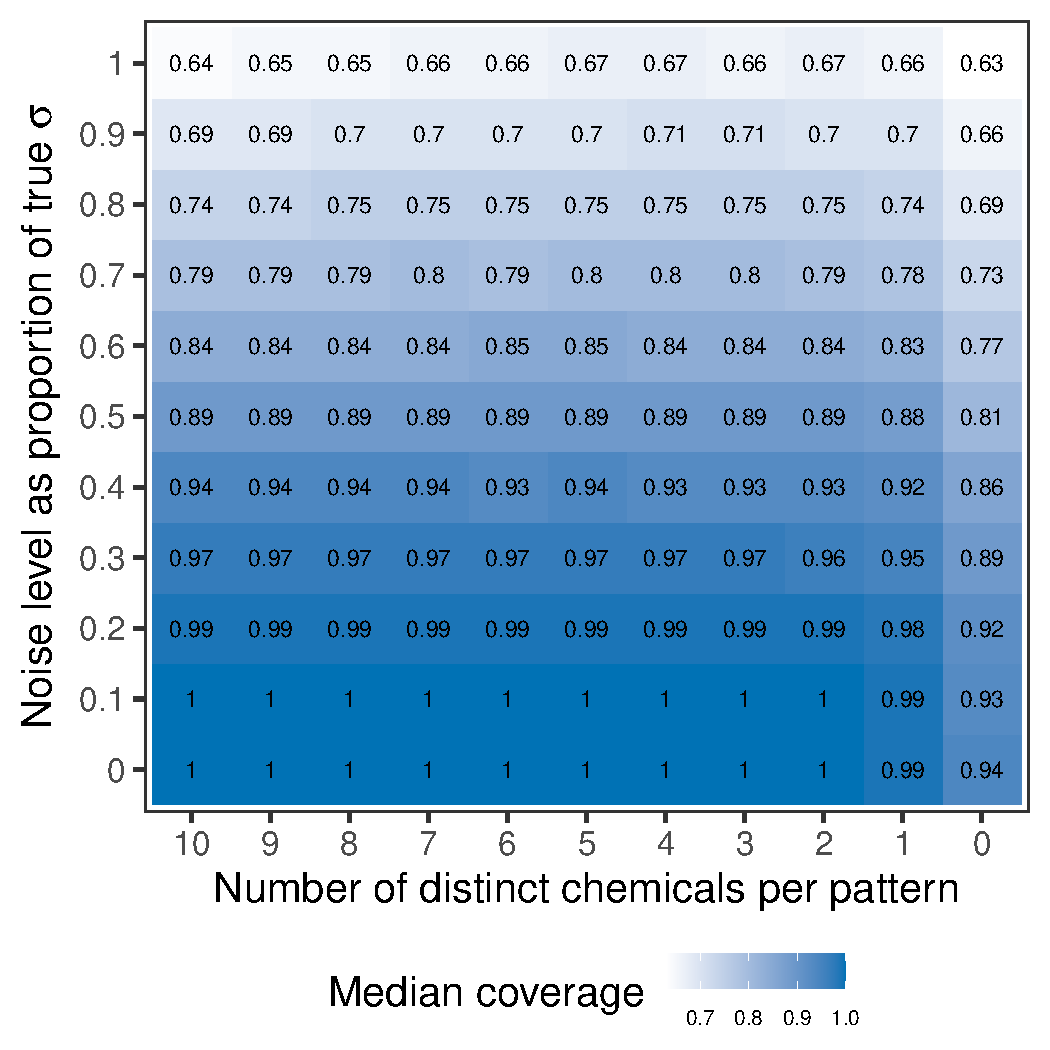
\includegraphics[scale = 0.7]{./figures/coverage_heat.pdf}
\end{figure}

\subsubsection{Variational confidence intervals}
Figure~\ref{heatmap} displays median coverage of variational confidence intervals for simulation scenarios taken across entries in 100 datasets per grid square, for all pattern structures and added noise levels. When the noise level was low and no chemicals loaded on multiple patterns, variational confidence intervals achieved 100\% coverage. As noise increased, coverage decreased, with added noise greater than or equal to $0.5 \times \sigma$ resulting in confidence intervals that did not achieve nominal coverage, i.e. did not include the true value 95\% of the time. As underlying patterns overlapped more, coverage again decreased, though notably less steeply than with increasing noise. At the extreme, with all patterns overlapping and added noise equal to $\sigma$, variational confidence intervals failed to include the true values almost 40\% of the time. This corresponds with poorer performance as the underlying structure became less separable. 

While variational confidence intervals only performed poorly in simulations with high noise, bootstrapped confidence intervals consistently performed much worse. Median coverage for bootstrapped \bnmf confidence intervals ranged from 0.06 at its worst (over distinct patterns and low noise) to 0.19 at its best (over overlapping patterns and low noise). Median coverage for bootstrapped confidence intervals is included in Supplemental Figure~\ref{fig:boot_coverage}. \bnmfc's variational confidence intervals were wider than bootstrapped confidence intervals 97\% of the time, indicating that \bnmf appropriately accounted for uncertainty in the coefficient matrix. The narrower bootstrapped confidence intervals imply that less uncertainty was due to randomness in the simulated data than in the model itself.

Variational confidence intervals derive from the distribution of $\hat{W}\operatorname{diag}(\hat{\mathbf{a}}) \sim \operatorname{Gamma}(\hat{\alpha}_W,$ $\hat{\beta}_W) \times \operatorname{Gamma}(\hat{\alpha}_\mathbf{a}, \hat{\beta}_\mathbf{a})$, which notably includes both tails of the distribution, whereas bootstrapped confidence intervals stem from the distribution of $\mathbb{E}\left[\hat{W}\operatorname{diag}(\hat{\mathbf{a}})\right]$ across bootstraps. Bootstraps generated similar expected values, which resulted in necessarily narrower confidence intervals. Bootstrapping, however, did provide wider confidence intervals for chemical loadings (85\% of the time). Supplemental Figure~\ref{fig:ci_dist} gives representative examples of differences between variational and bootstrapped confidence intervals. We additionally included comparisons with bootstrapped confidence intervals for Poisson NMF in Supplemental Figures~\ref{fig:ci_dist} and \ref{fig:boot_coverage}.

\subsection{Secondary simulations}
These findings largely held in sensitivity analyses with varying dimensions. Simulated datasets with larger sample sizes had higher coverage and lower error, on average, when compared with smaller $N$. Conversely, simulations with larger mixture sizes had lower coverage and higher error, on average, when compare with smaller $P$. Supplemental Figure~\ref{fig:dim_coverage} depicts \bnmf coverage over noise level and separability of patterns across sample and mixture sizes.

The number of patterns affected performance less consistently. \bnmf performed poorly on simulations with one underlying pattern, indicating that \bnmf is not an appropriate method when building a scale or index. PCA, on the other hand, performed much better with only one true pattern. Factor analysis chose the correct number for all simulations with one underlying pattern and chose a ten pattern solution in all but 1.3\% of simulations with ten distinct underlying patterns. On simulations with ten overlapping patterns, performance decreased drastically across all methods. Factor analysis performed the best, estimating the correct number of patterns for 60.8\% of simulations with low noise, but its success rate dropped to 8.9\% for simulations with high noise.

Accurate estimation of the underlying number of patterns in these secondary simulations is quantified in Supplemental Table~\ref{tab_rank} as the proportion of simulations for which \bnmfc, NMF, factor analysis, and PCA estimated the correct pattern number. Supplemental Figure~\ref{fig:pattern_coverage} depicts \bnmf coverage over noise level and separability of patterns across values of $K$. We present relative error for predicted values and estimated scores across sample and mixture sizes for $K$ = 1, 4, and 10 in Supplemental Tables~\ref{table:sup1}, \ref{table:sup4}, and \ref{table:sup10}, respectively.

\subsection[Application]{Application to a mixture of endocrine disrupting chemicals in pregnant women}
\label{results_app}
Primary data from 727 pregnant women ages 18--35 were collected as part of the Columbia Center for Children's Environmental Health's Mothers and Newborns longitudinal birth cohort. This mother-child cohort was initiated to evaluate the effects of prenatal exposure to environmental contaminants on birth outcomes and child development \cite{perera2006effect}. Multiple potential EDCs were measured in spot urine samples collected during the third trimester in a subset of 343 mothers \cite{factor2014persistent}. Here, we evaluated a mixture of 17 chemicals from two classes: nine phthalate metabolites and eight phenols. Concentrations below the limit of detection (LOD) were assigned a value of LOD/$\sqrt{2}$ \cite{hornung1990estimation}. All chemical concentrations were specific gravity-adjusted to account for urinary dilution \cite{hauser2004temporal}. Exposures were scaled by their standard deviation but not mean-centered, to retain non-negativity.

Exposure levels of phthalates were generally positively correlated, though the majority of correlations (70\%) were weak (between 0.0 and 0.3). Four phthalate metabolites (MEHHP, MECPP, MEOHP, and MEHP) from the same parent compound had correlation coefficients $>$ 0.7. Phenols displayed lower within-class correlations, with the exception of 24-DCP and 25-DCP ($r$ = 0.94) and PPB and MPB ($r$ = 0.75). Notable between-class correlations include MEP's moderate correlation with two phenols ($r > 0.4$) and BPA's moderate correlations with four phthalates ($r > 0.2$).

\begin{landscape}
\begin{figure}
\centering
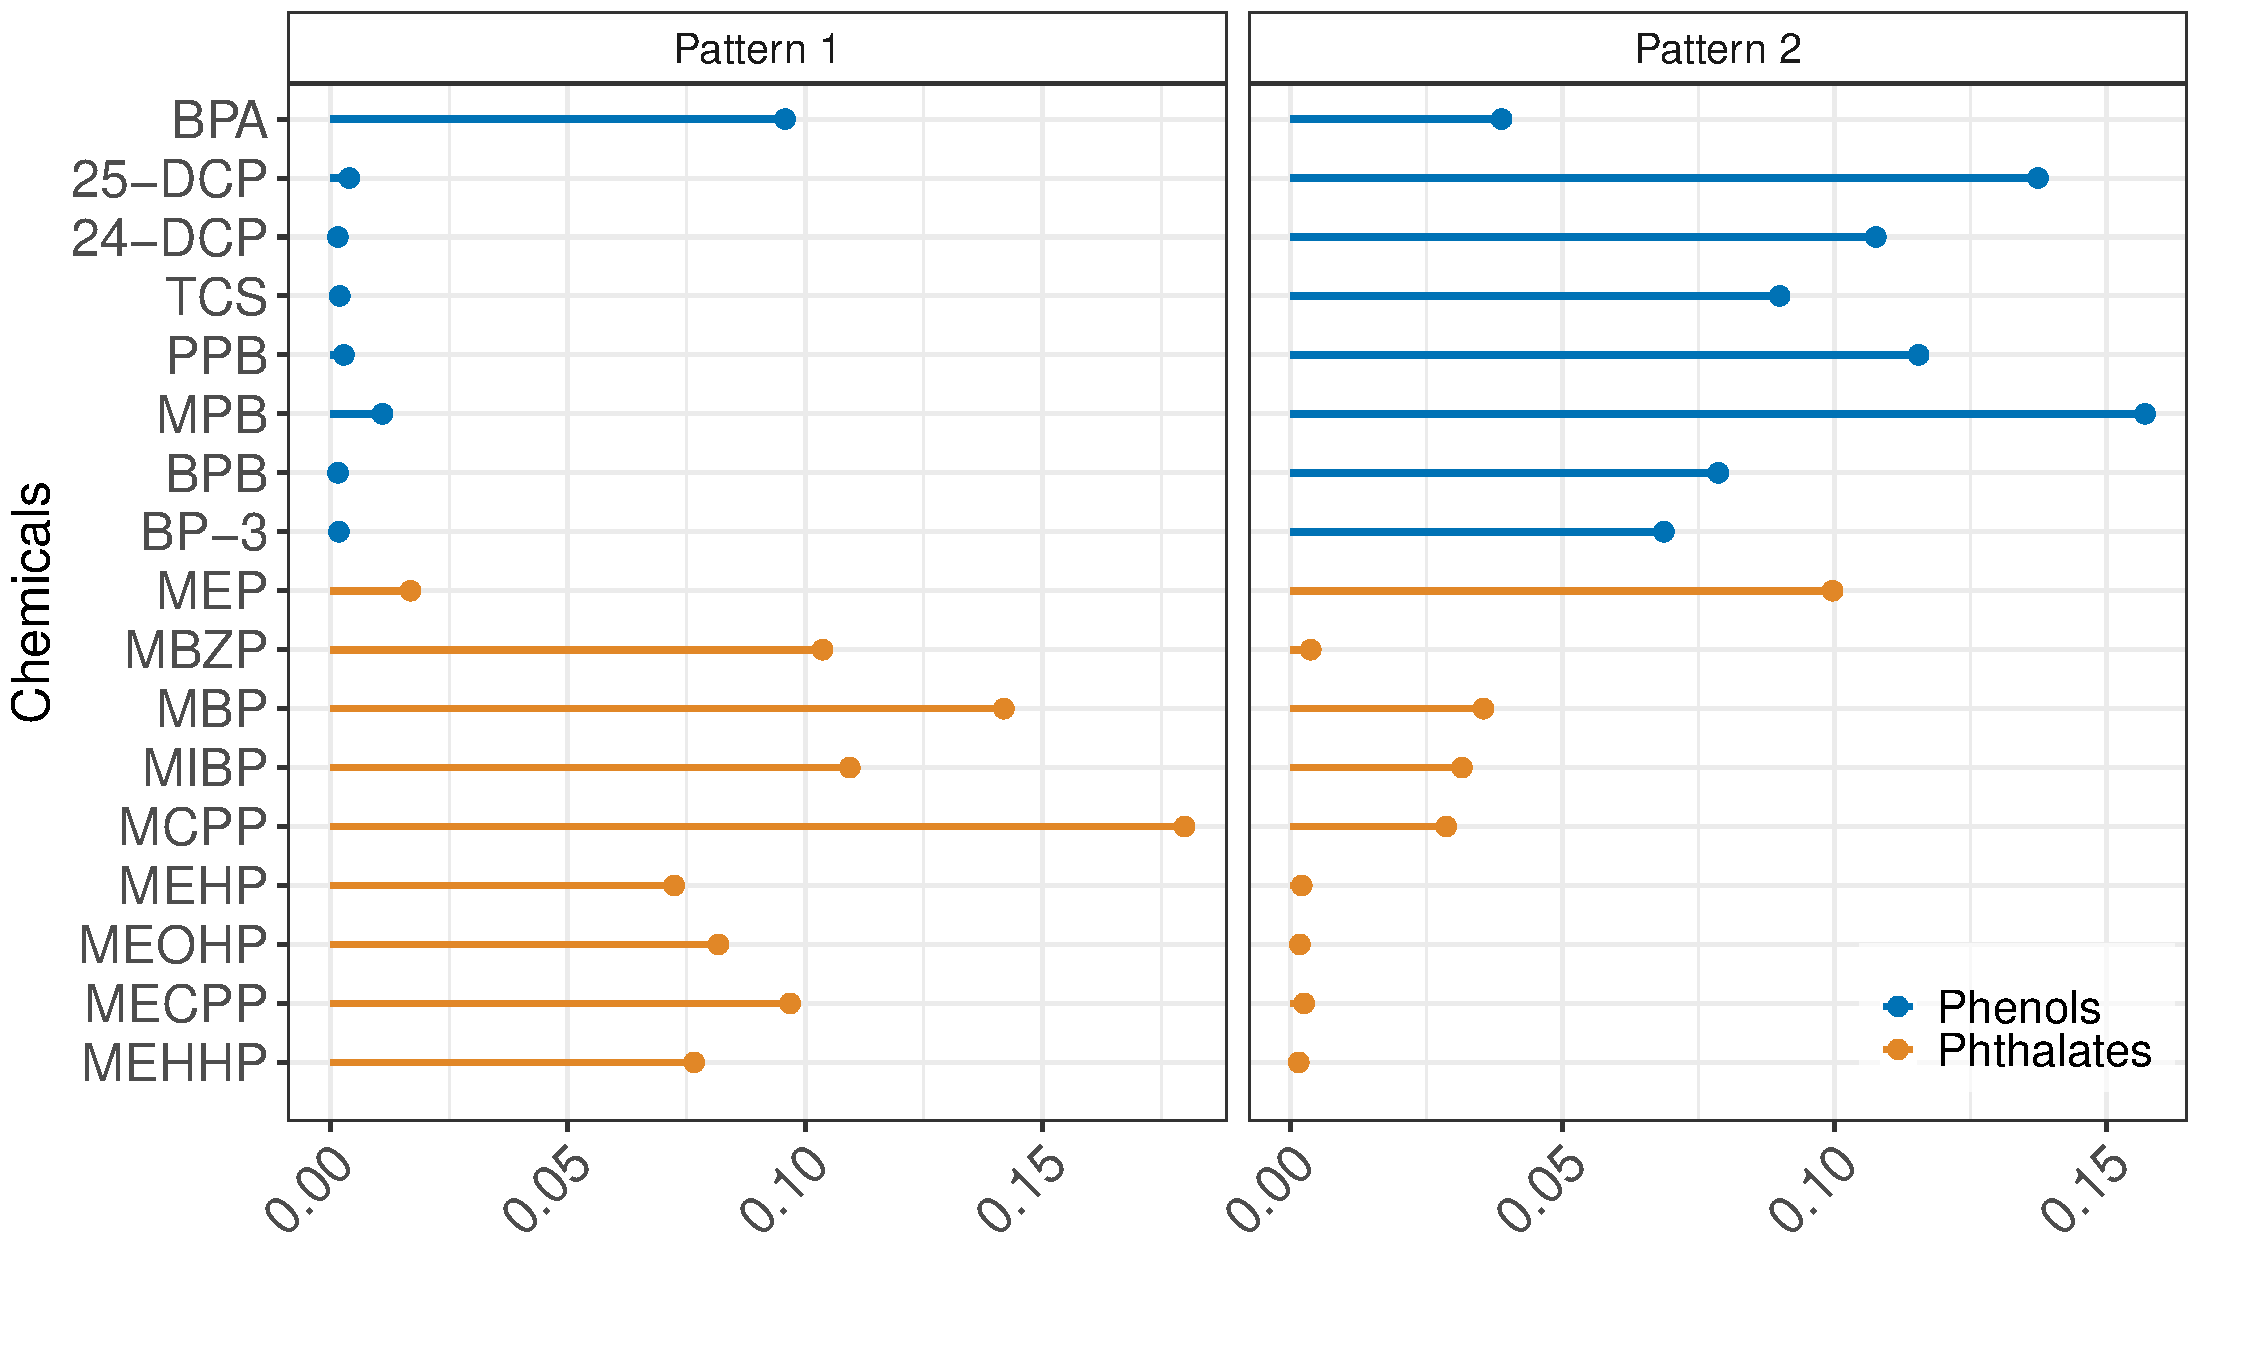
\includegraphics[scale = 0.55]{./figures/mn2_edc_loadings_flip.pdf}
\caption[Patterns of EDC exposure in Mothers and Newborns cohort]{Patterns of potentially endocrine disrupting chemical exposure in pregnant women identified by \bnmf in a mixture of 17 phenols and phthalates. Patterns generally correspond with dietary exposures (pattern 1) and personal care product exposures (pattern 2).}
\label{fig:patterns}
\end{figure}
\end{landscape}

\begin{landscape}
\begin{figure}
\centering
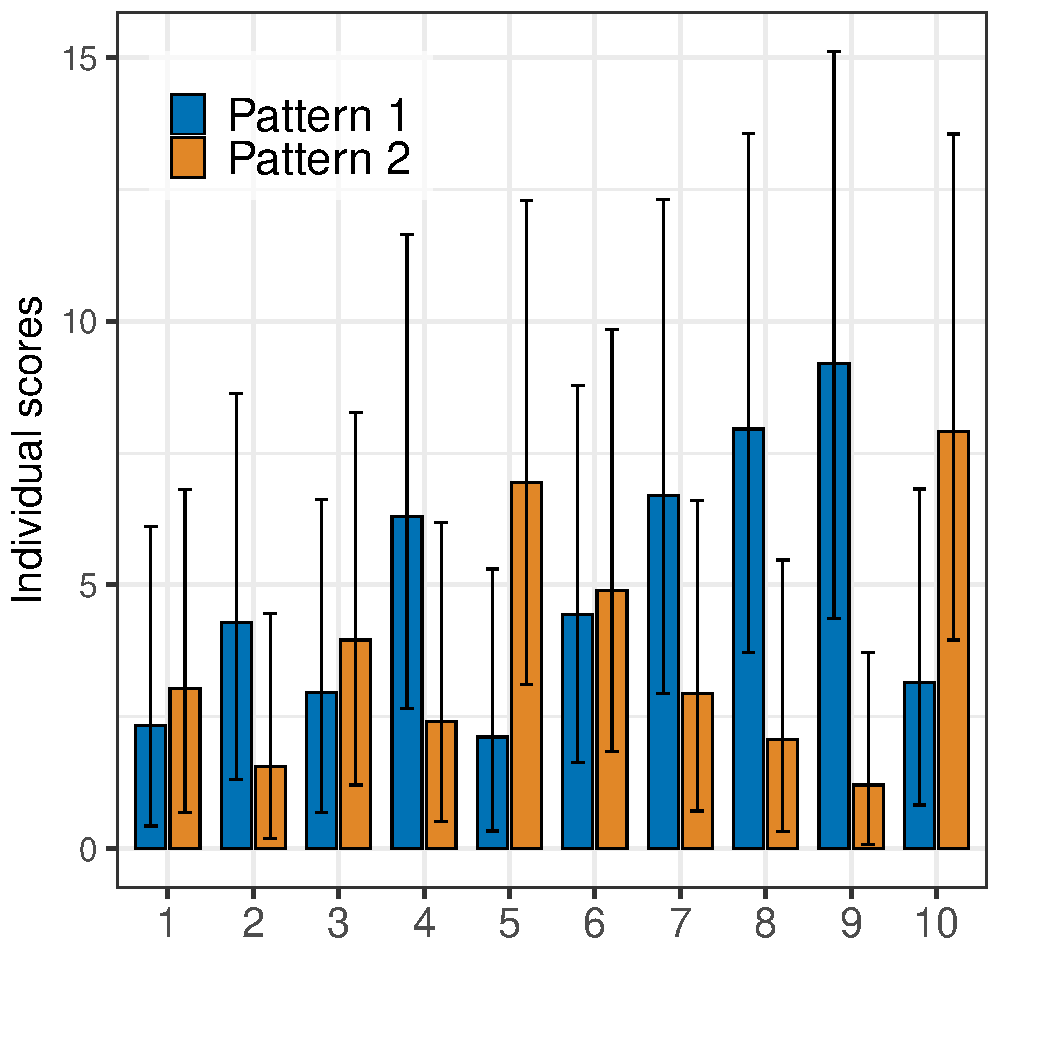
\includegraphics[scale = 0.75]{./figures/scores_w_vci.pdf}
\caption[Individual scores and variational confidence intervals]{Individual scores and 95\% variational confidence intervals on \bnmfc-identified patterns for a random subset of ten participants in the Mothers \& Newborns cohort. This shows variability across individual pattern scores and across patterns within individuals. Error bars span the upper and lower bounds of the 95\% variational confidence intervals, which display uncertainty in the estimation of individual scores.}
\label{fig:scores}
\end{figure}
\end{landscape}

As preliminary analyses, we fit PCA and NMF on the exposure concentrations. For PCA, we chose 11 principal components that explained 80\% of the variance in the data. For NMF, we chose a one factor model based on BIC. The identified factor loadings expressed common exposure to all chemicals, without distinguishing separate patterns.

We then applied \bnmf to identify exposure patterns of phenols and phthalates in pregnant women without specifying the number of patterns. We ran 100 models using variational inference (described in Section \ref{methods_vi}), and chose the run with the largest objective value for inference. \bnmf identified two patterns of EDC exposure: (1) majority phthalates, and (2) majority phenols. Two notable cross-class loadings occurred; MEP loaded with phenols, and BPA loaded with phthalates. These groupings may be explained by potential shared predominant exposure routes through personal care products (phenols and MEP) and diet (phthalates and BPA). Pattern loadings are shown in Figure~\ref{fig:patterns}. 

We also obtained variational confidence intervals around individual scores, which may be included in a health model. Each individual score had its own mean and variance. Score means across all individuals averaged 5.3 ng/ml (between person standard deviation (sd) = 4.4) for pattern 1 and 4.7 ng/ml (sd = 3.4) for pattern 2, ranging from 1.1 to 44.5 ng/ml and 1.0 to 20.3 ng/ml, respectively. The average within-person variance of individual scores averaged 4.5 for pattern 1 and 3.9 for pattern 2, ranging from 0.9 to 38.6 and 0.9 to 17.0, respectively. We depict confidence intervals around a random subset of individual scores in Figure~\ref{fig:scores}.

\section{Discussion}

We have proposed \bnmf as a new approach to identify patterns of chemical exposures in environmental mixtures. Our simulation studies highlight two main advantages of \bnmf over existing frequentist approaches. First, by fitting a non-parametric prior on the number of patterns in a mixture, \bnmf helps to remove the researcher from the specification and selection of $K$. To our knowledge, all methods currently utilized in environmental health research require an \textit{a priori} specification or \textit{post-hoc} selection of pattern number. Second, the Bayesian framework allows us to estimate 95\% variational confidence intervals surrounding point estimates for individual scores. Coverage of true individual scores was $>$95\%, on average, when added noise was below 40\% in our simulations. Variational confidence intervals better capture uncertainty in inference and may aid researchers in the interpretation of results, especially if, for example, uncertainty is not the same across patterns or across individuals. Quantification of confidence may also be included in two-stage analyses, which could help in obtaining more comparable results across studies. Health models that ignore this uncertainty may have overly narrow confidence intervals and unstable effect estimates, threatening inference \cite{mak14_unc}.

In an application of \bnmf to real-life data, we found two patterns of EDCs in a cohort of pregnant women. While we do not know the true exposure sources or the data generating process in this example, the identified patterns can be interpreted as two exposure routes or sources. One pattern of exposure to seven phenols and one phthalate metabolite, MEP, aggregated EDCs whose primary exposure route is through personal care products. Phenols are used as plasticizers, antibacterial agents, and preservatives in a wide variety of personal care products \cite{philippat2015exposure}, and MEP is primarily found in fragrances \cite{koniecki2011phthalates}. The second pattern combined the remaining eight phthalates and BPA. The majority of these phthalates are metabolites of compounds found in food packaging \cite{schettler2006human}. BPA is also found in packaging, such as the lining of aluminium cans, and both phthalates and BPA are known to leach into food \cite{vandenberg2007human}. \bnmfc-identified variational confidence intervals further allowed for uncertainty characterization. For example, while variational confidence intervals exhibited substantial overlap across individuals, within-participant variances on patterns 1 and 2 were often quite disparate, indicating more confidence in one score than the other. This application shows \bnmf as a useful tool to identify exposure patterns in environmental mixtures. 

The primary and secondary simulations were implemented to describe a variety of potential contexts in which pattern recognition methods may be desired in environmental health research. We simulated settings ranging from distinct to overlapping patterns. We varied the number of patterns (1, 4, and 10), number of study subjects (200, 1,000, 10,000), and number of features (20, 40, and 100). We adjusted the inter-chemical correlations and the amount of added noise. \bnmf performed comparably with more commonly used methods on a number of metrics. However, there remain high-dimensional application areas, such as epigenetics or metabolomics, that are not well represented by our simulations. Computationally, the sample size and dimension of the exposure vector behave as limiting factors in these models, though the variational inference algorithm was written to enhance efficiency and may be further extended to a stochastic version to facilitate larger $N$ or $P$.

Bayesian methods may be sensitive to prior specifications. We chose Gamma priors on chemical loadings, individual scores, and the number of patterns because of their aptness in the setting of environmental concentrations. The Gamma distribution is non-negative and continuous (as are environmental exposures), with support $x \in (0, \infty)$, and finite mean and variance appropriate for real-life data. We specified $\operatorname{Gamma}(\alpha = \mathbf{1}, \beta = \mathbf{1})$ as a weakly informative distribution over our prior beliefs for the coefficient and dictionary matrices. This prior reflects a belief that is weakly held and easily molded by exposure to new information from empirical observations. We stipulated $\operatorname{Gamma}(\alpha = \frac{1}{K}, \beta = 1)$ to enforce sparsity on the number of patterns discovered.

Variational inference provides an accurate approximation of the full posterior distribution. Still, it is generally not recommended to infer properties of an underlying distribution beyond the expected value due to the difficulty in verifying the assumptions regarding the factorization of the posterior distribution. This begs the question, why not simulate \bnmfc's posterior distribution with a Markov chain Monte Carlo (MCMC)? Several considerations led us to prefer variational inference over MCMC for \bnmfc. First, we developed \bnmf primarily for use in environmental mixtures analyses, often performed by environmental epidemiologists. Variational inference is a more approachable method for many researchers. Pragmatically, by converting the inference problem into an optimization problem, variational inference outperforms MCMC in terms of analytic efficiency. An MCMC is more computationally intense and often assumes access to higher performance computing resources. Additionally, research on bounds for guaranteed MCMC mixing time is, in general, an open area \cite{levin2017markov}, which places the burden of assessing convergence on the end user. This is not a trivial task, especially for users without formal training, and variational inference avoids it by converging to a local minimum. Multiple runs of variational inference are easily ranked in terms of performance; the model that obtains the highest objective value is the best approximation of the true posterior distribution. In this way, variational inference is more widely usable. 

A second consideration was the complexity of the model at hand. Because of the nonparametric prior on the number of patterns in $\mathbf{a}$, \bnmf is not conjugate, thus requiring a more complex MCMC than a Gibbs sampler. This, in itself, did not make an MCMC impractical, but the nonparametric prior created an additional difficulty wherein samples within the same chain could result in different numbers of patterns, complicating the Monte Carlo step.

An MCMC would further suffer from label switching, which makes the posterior distribution non-identifiable. The posterior distribution is invariant to permutations of the labels of patterns $1 ... K$. Label switching occurs when the pattern labels permute \cite{celeux1998bayesian}, resulting in an uninterpretable posterior. While there are certain proposed approaches to address this issue, such as parameter ordering constraints or relabeling strategies \cite{rodriguez2014label}, there are no consensus solutions \cite{gelman06}. Variational inference sidesteps label switching though iterative optimization; the patterns inferred in the first iteration initialize the next iteration, resulting in a sequence of improving approximations.

We show in Figure~\ref{heatmap} that as long as separability holds, \bnmfc's variational confidence intervals achieves nominal coverage or better. In fact, even when patterns were assumed to be known (i.e. with zero error in dictionary matrix estimation), both the error in coefficient matrix estimation and variational confidence interval coverage decreased as noise was added (results not shown), indicating that declines in performance were due to a loss of separability and not to a deficiency of variational inference. In fact, variational confidence intervals consistently performed better than bootstrapped confidence intervals, which never achieved nominal coverage.

In Section~\ref{methods_bayesian} we described the probabilistic interpretation on which \bnmf was built. It began with modeling the data as independent random variables and drawing latent variables independently from Gamma priors \cite{cemgil2008bayesian, paisley2014bayesian}. Variational inference, likewise, models latent variables as mutually independent and governed by a distinct factor in the variational density \cite{blei2017variational}. In this way, assumptions of variational inference cohere with assumptions of the data generating process of all NMF methods, including \bnmf.

\bnmf performed comparably to other pattern identification methods in simulations across several metrics of error in magnitude of values and direction of patterns. \bnmf and frequentist NMF have the advantage over factor analysis and PCA of returning solution matrices on immediately interpretable scales. For example, in our EDC application, chemicals were measured in nanograms of a chemical per milliliter of urine. After non-negative decomposition, individual scores were represented as nanograms of a pattern per milliliter of urine, and chemical loadings were represented as nanograms of a chemical per nanogram of a pattern. PCA and factor analysis have no such intuitive framing.

\bnmf had additional benefits over frequentist NMF. Although they performed similarly in simulations, when we applied them to real-life data and used BIC to choose the optimal model, both NMF with an $\ell_2$ penalty and with a Poisson likelihood returned a single factor. Since the goal of the analysis was to identify patterns that could be interpreted as chemical sources and not to create an index of chemical exposures, a single factor failed to address the research question. Additionally, bootstrapped confidence intervals around individual scores from NMF (see Supplemental Figure~\ref{fig:boot_coverage}) performed substantially worse than variational confidence intervals, even when simulated noise was low, indicating that the posterior distribution of \bnmf better encapsulate the truth than the maximum likelihood analog.

With this work we aimed to improve reproducibility and robustness of pattern identification in environmental health. We incorporated a non-parametric sparse prior in a Bayesian model to estimate the number of patterns in high-dimensional environmental mixtures. This approach may aid researchers in model selection. Additionally, the Bayesian formulation allows for uncertainty quantification. \bnmf may be used as a feature selection step in a Bayesian two-stage analysis incorporating individual pattern scores and distributions as exposures in subsequent health models. Our model achieved nominal coverage even with moderate noise. In future work, we will build the hierarchical Bayesian health model and consider useful extensions, such as 1) a fully supervised model where the health outcome informs pattern identification, and 2) accounting for clustered information, e.g. repeated measurements or geographical clustering.

{\setcounter{figure}{0} % put supplemental numbering in curly braces
\setcounter{table}{0}
\renewcommand{\thefigure}{3.S.\arabic{figure}}
\renewcommand{\thetable}{3.S.\arabic{table}}
\clearpage
\section{Supplementary Material}
\label{sec6}

\subsection{Bootstrapped confidence intervals}
\begin{figure}[!h]
\caption[Comparison of variational and bootstrapped confidence intervals]{Example distributions for variational and bootstrapped 95\% confidence intervals of \bnmf and bootstrapped 95\% confidence intervals of NMF with the Poisson likelihood. Histograms show full distributions for these three distributions over a single entry in each solution matrix, i.e., an individual's estimated score on one pattern ($\mathbb{E}[W_{i k}\mathbf{a_k}]$), a chemical's estimated loading on one pattern ($\mathbb{E}[H_{k j}]$), and an individual's predicted value for one chemical ($\mathbb{E}[W_{i k}\mathbf{a}_k]*\mathbb{E}[H_{k j}]$). Dashed black lines represent the true value. Dashed colored lines represent the variational mean (blue), bootstrapped \bnmf median (red), and bootstrapped NMF median (green). Dotted colored lines represent the 95\% confidence intervals.}
\label{fig:ci_dist}
\centering
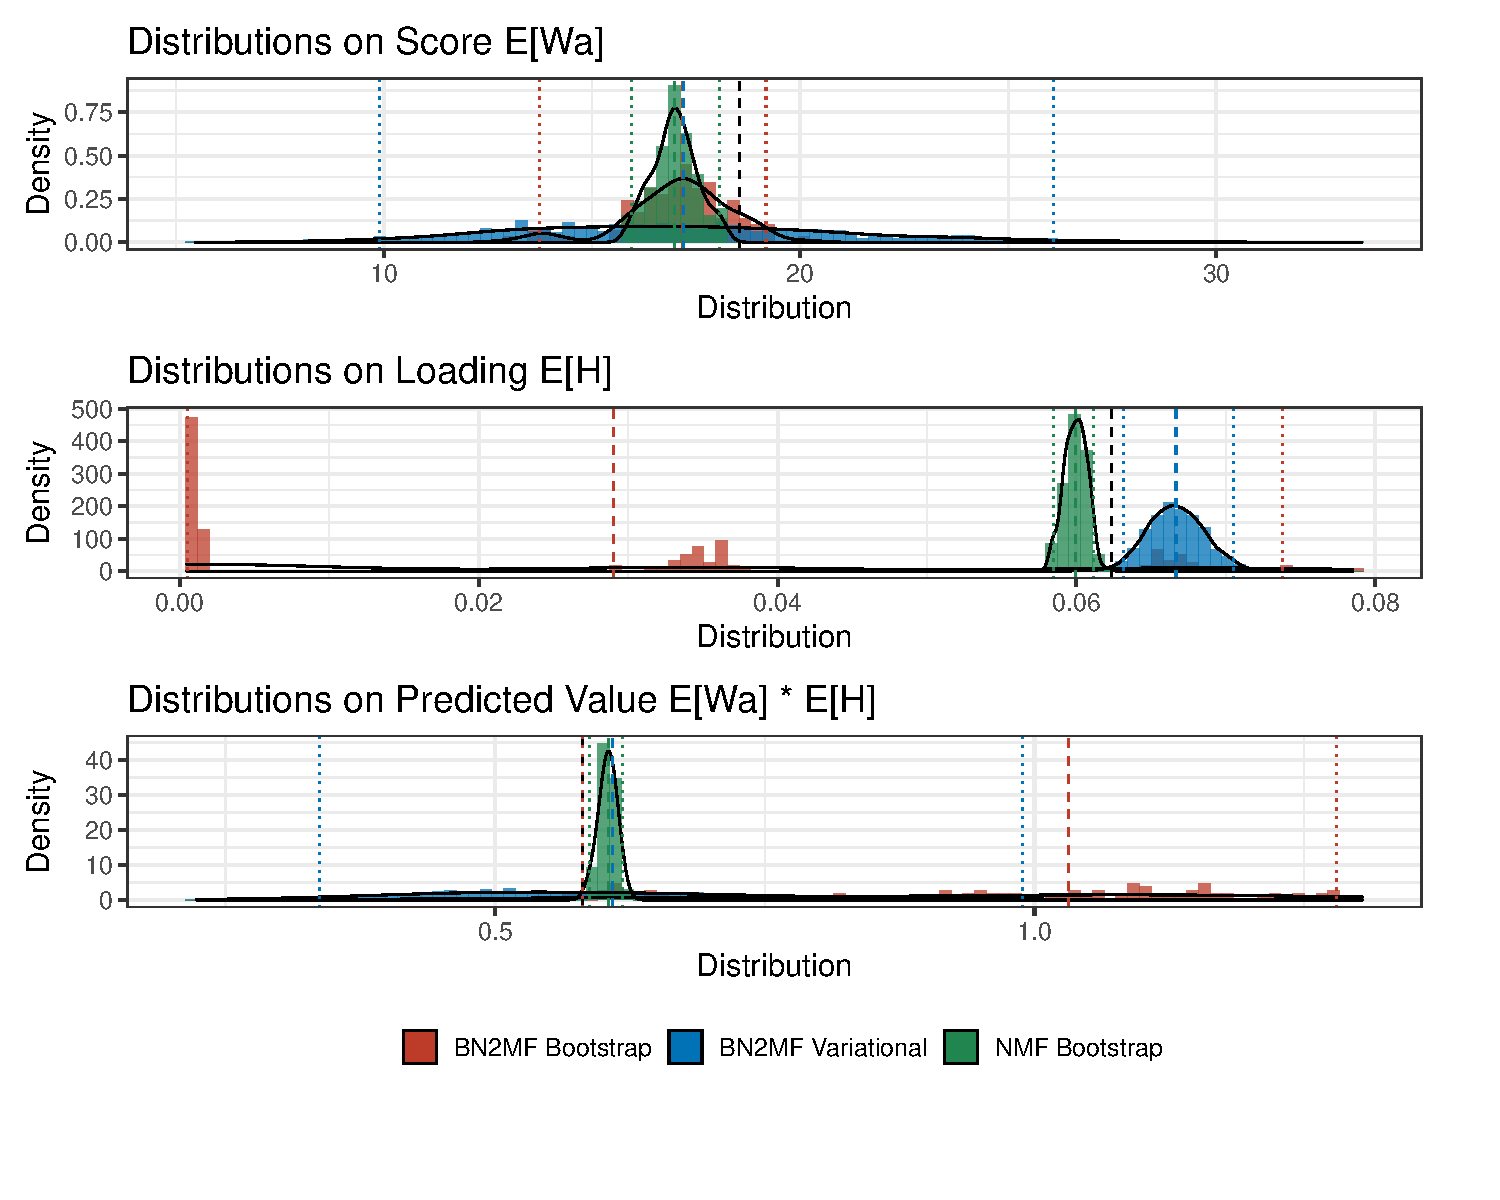
\includegraphics[scale = 0.65]{./figures/vci_bci_nmfci.pdf}
\end{figure}

\clearpage
\begin{figure}
\caption[Comparison of variational and bootstrapped coverage]{Ninety-five percent confidence interval coverage for variational confidence intervals, bootstrapped \bnmf confidence intervals, and bootstrapped Poisson NMF confidence intervals. Each square represents simulation that estimated a 4 pattern solution, colored according to median coverage (proportion of true values within estimated 95\% variational confidence intervals). On the x axis, number of distinct chemicals per pattern is 10 (distinct) or 0 (overlapping). On the y axis, added noise level relative to the true standard deviation increases from 0.2 (low added noise) to 1 (as much added noise as true noise).}
\label{fig:boot_coverage}
\centering
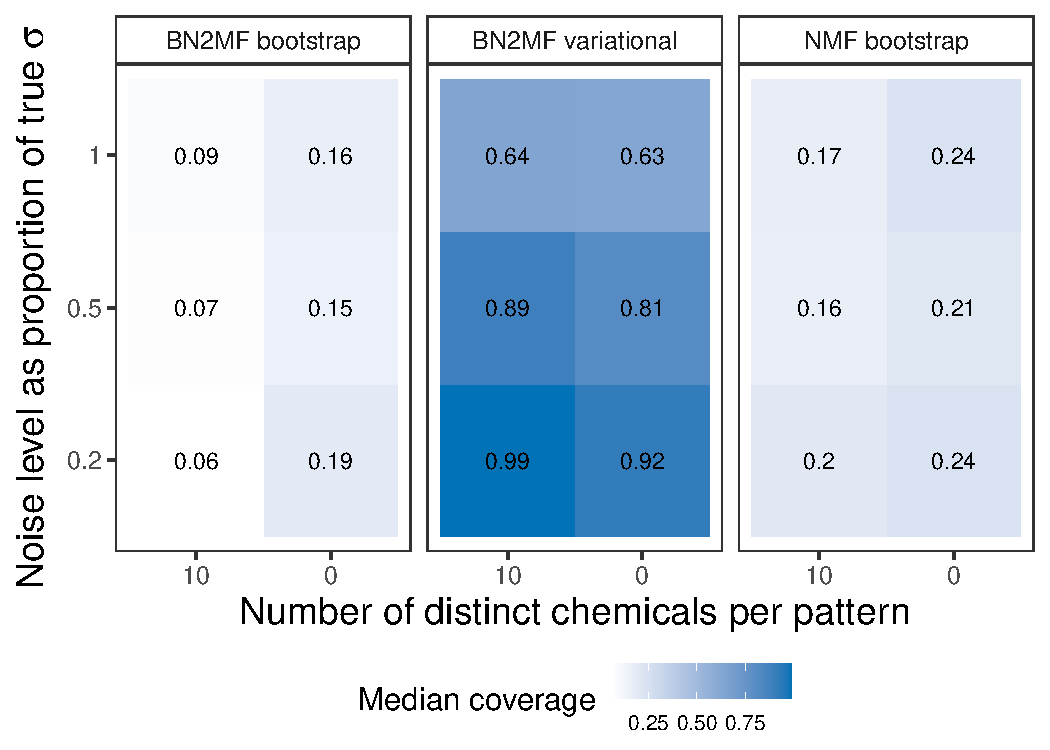
\includegraphics[scale = 0.7]{./figures/bootstrap_coverage.pdf}
\end{figure}

\clearpage
\subsection{Secondary analyses varying $N$, $P$, and $K$}
\subsubsection{Estimation of $K$}
%\hspace{5ex}
\begingroup
\renewcommand{\arraystretch}{1.25}
\begin{table}[!h] \centering 
  \caption[Estimation of $K$ by \bnmf and comparison models]{Percentage of correct estimation of number of patterns describing underlying matrices in secondary simulations. Percentages were taken across 900 simulated datasets (100 datasets of each possible combination of sample sizes (200, 1,000, and 10,000) and mixture sizes (20, 40, and 100). $^*$ FA = factor analysis; NMF-$\ell_2$ = NMF with $\ell_2$ penalty; NMF-P = NMF with Poisson likelihood.} 
  \label{tab_rank}
  \addtolength{\tabcolsep}{-2pt}
\begin{tabular}{lrrr|rr}
\multicolumn{6}{c}{Correct Pattern Number Estimation} \\
\hline 
\hline  
& \multicolumn{3}{c}{Distinct Patterns} & \multicolumn{2}{c}{Overlapping} \\
\hline
\hline  
Model$^*$ & \multicolumn{1}{c}{Rank 1} & \multicolumn{1}{c}{Rank 4} &  \multicolumn{1}{c}{Rank 10} &  \multicolumn{1}{c}{Rank 4} & \multicolumn{1}{c}{Rank 10} \\ 
\hline
\hline  
& \multicolumn{5}{c}{Simulations + 20\% Noise} \\
\hline
\bnmf        &  1.6 & 100.0 & 66.6 & 82.7 & 11.3 \\ 
FA           &  100.0 & 100.0 & 100.0 & 100.0 & 60.8 \\ 
NMF-$\ell_2$ &  100.0 & 100.0 & 92.6 & 70.3 & 0.0 \\ 
NMF-P        &  97.8 & 100.0 & 94.7 & 76.2 & 0.0 \\ 
PCA          &  100.0 & 69.9 & 20.0 & 0.0 & 0.0 \\ 
\hline  
& \multicolumn{5}{c}{Simulations + 50\% Noise} \\
\hline
\bnmf        & 0.0 & 100.0 & 68.2 & 85.2 & 11.6 \\ 
FA           & 100.0 & 100.0 & 100.0 & 100.0 & 28.3 \\ 
NMF-$\ell_2$ & 95.0 & 100.0 & 93.1 & 73.7 & 0.0 \\ 
NMF-P        & 43.6 & 100.0 & 94.9 & 78.0 & 0.0 \\ 
PCA          & 2.8 & 99.3 & 11.3 & 79.3 & 11.8 \\ 
\hline  
& \multicolumn{5}{c}{Simulations + 100\% Noise} \\
\hline
\bnmf        & 0.0 & 87.4 & 81.1 & 90.2 & 16.9 \\ 
FA           & 100.0 & 100.0 & 96.3 & 95.7 & 8.9 \\ 
NMF-$\ell_2$ & 30.7 & 86.3 & 85.3 & 81.7 & 0.4 \\ 
NMF-P        &  3.6 & 93.1 & 87.0 & 83.1 & 1.1 \\ 
PCA          & 0.0 & 0.0 & 0.0 & 0.0 & 0.0 \\ 
\hline \\[-1.8ex] 
\end{tabular} 
\end{table} 
\endgroup

\clearpage
\begingroup
\renewcommand{\arraystretch}{1.35}
\begin{table}[!htbp] \centering 
  \caption[Relative error for rank 1 secondary simulations]{Relative error for predicted values and individual scores of rank 1 secondary simulation with + 20\% noise. Values presented are mean (standard deviation). Error was averaged over 100 simulations for each combination of sample size ($N$ = 200, 10,000), mixture size ($P$ = 20, 40, 100) and simulation strategy (distinct or overlapping patterns). Entries marked as ``---'' indicate that no models on that group of simulations correctly identified the number of patterns, and error on scores could not be computed. $^*$ FA = factor analysis; NMF-$\ell_2$ = NMF with $\ell_2$ penalty; NMF-P = NMF with Poisson likelihood. $^+$ $N$ = sample size.}
  \label{table:sup1} 
 \addtolength{\tabcolsep}{-2pt}
\begin{tabular}{lrr|rr}
\multicolumn{5}{c}{Relative Error for Rank 1 Secondary Simulations with + 20\% Noise} \\
\hline 
\hline  
& \multicolumn{2}{c}{Predicted Values} & \multicolumn{2}{c}{Estimated Individual Scores} \\
\hline
\hline  
Model$^*$ & \multicolumn{1}{c}{$N^+$ = 200} & \multicolumn{1}{c}{$N$ = 10,000} & \multicolumn{1}{c}{$N$ = 200} & \multicolumn{1}{c}{$N$ = 10,000} \\
\hline
\hline  
& \multicolumn{4}{c}{Mixture size $P$ = 20} \\
\hline
BN2MF & 0.21 (0.01) & 0.22 ($<$0.01) & --- & --- \\ 
FA & 0.44 (0.09) & 0.49 (0.02) & 0.75 (0.02) & 0.75 ($<$0.01) \\ 
NMFL2 & 0.17 (0.01) & 0.17 ($<$0.01) & 1.00 ($<$0.01) & 1.00 ($<$0.01) \\ 
NMFP & 0.27 (0.03) & 0.30 (0.01) & 3.07 (0.85) & 11.46 (3.22) \\ 
PCA & 0.23 (0.01) & 0.23 ($<$0.01) & 1.84 (0.07) & --- \\ 
\hline 
& \multicolumn{4}{c}{Mixture size $P$ = 40} \\
\hline 
BN2MF & 0.19 (0.01) & 0.20 ($<$0.01) & --- & --- \\ 
FA & 0.44 (0.09) & 0.49 (0.02) & 0.75 (0.02) & 0.75 ($<$0.01) \\ 
NMFL2 & 0.15 (0.02) & 0.15 ($<$0.01) & 1.00 ($<$0.01) & 1.00 ($<$0.01) \\ 
NMFP & 0.23 (0.03) & 0.21 (0.04) & 2.80 (0.65) & 9.30 (1.92) \\ 
PCA & 0.22 (0.01) & 0.22 ($<$0.01) & 3.01 (0.08) & --- \\ 
\hline 
& \multicolumn{4}{c}{Mixture size $P$ = 100} \\
\hline 
BN2MF & 0.18 (0.01) & 0.18 ($<$0.01) & --- & --- \\ 
FA & 0.44 (0.09) & 0.49 (0.02) & 0.75 (0.02) & 0.74 ($<$0.01) \\ 
NMFL2 & 0.14 (0.02) & 0.14 (0.01) & 1.00 ($<$0.01) & 1.00 ($<$0.01) \\ 
NMFP & 0.19 (0.02) & 0.18 ($<$0.01) & 2.49 (0.55) & --- \\ 
PCA & 0.22 (0.01) & 0.22 ($<$0.01) & --- & --- \\ 
\hline
\hline  
\end{tabular}
\end{table}
\endgroup

\clearpage
\begin{landscape}
\begingroup
\renewcommand{\arraystretch}{1.2}
\begin{table}[!htbp] \centering 
  \caption[Relative error for rank 4 secondary simulations]{Relative error for predicted values and estimated individual scores of rank 4 secondary simulation with + 20\% noise. Values presented are mean (standard deviation). Error was averaged over 100 simulations for each combination of sample size ($N$ = 200, 10,000), mixture size ($P$ = 20, 40, 100) and simulation strategy (distinct or overlapping patterns). $^*$ FA = factor analysis; NMF-$\ell_2$ = NMF with $\ell_2$ penalty; NMF-P = NMF with Poisson likelihood. $^+$ $N$ = sample size.}
  \label{table:sup4} 
 \addtolength{\tabcolsep}{-2pt}
\small
\begin{tabular}{lrr|rr|rr|rr}
\multicolumn{9}{c}{Relative Error for Rank 4 Secondary Simulations with + 20\% Noise} \\
\hline 
\hline  
& \multicolumn{4}{c}{Predicted Values} & \multicolumn{4}{c}{Estimated Individual Scores} \\
\hline
\hline
& \multicolumn{2}{c}{Distinct Patterns} & \multicolumn{2}{c}{Overlapping Patterns} & \multicolumn{2}{c}{Distinct Patterns} & \multicolumn{2}{c}{Overlapping Patterns} \\
\hline
\hline  
Model$^*$ & \multicolumn{1}{c}{$N^+$ = 200} & \multicolumn{1}{c}{$N$ = 10,000} & \multicolumn{1}{c}{$N$ = 200} & \multicolumn{1}{c}{$N$ = 10,000} & \multicolumn{1}{c}{$N$ = 200} & \multicolumn{1}{c}{$N$ = 10,000} & \multicolumn{1}{c}{$N$ = 200} & \multicolumn{1}{c}{$N$ = 10,000} \\
\hline
\hline  
& \multicolumn{8}{c}{Mixture size $P$ = 20} \\
\hline
BN2MF & 0.18 (0.01) & 0.18 ($<$0.01) & 0.22 (0.04) & 0.18 (0.03) & 0.76 ($<$0.01) & 0.94 (0.05) & 0.80 (0.02) & 0.87 (0.04) \\ 
FA & 0.47 (0.05) & 0.48 (0.01) & 0.34 (0.06) & 0.34 (0.02) & 0.76 (0.01) & 0.75 ($<$0.01) & 0.79 (0.01) & 0.79 (0.01) \\ 
NMFL2 & 0.17 (0.01) & 0.16 ($<$0.01) & 0.20 (0.03) & 0.22 (0.03) & 1.00 ($<$0.01) & 1.00 ($<$0.01) & 1.00 ($<$0.01) & 1.00 ($<$0.01) \\ 
NMFP & 0.17 (0.01) & 0.16 ($<$0.01) & 0.20 (0.03) & 0.22 (0.04) & 6.80 (2.46) & 18.80 (5.89) & 5.10 (1.96) & 16.66 (6.39) \\ 
PCA & 0.18 (0.02) & 0.16 ($<$0.01) & 0.19 (0.03) & 0.17 (0.03) & 1.25 (0.07) & 1.23 (0.06) & 1.15 (0.06) & 1.23 (0.03) \\ 
\hline 
& \multicolumn{8}{c}{Mixture size $P$ = 40} \\
\hline 
BN2MF & 0.14 (0.01) & 0.13 ($<$0.01) & 0.15 (0.04) & 0.12 ($<$0.01) & 0.75 (0.02) & 0.90 (0.04) & 0.77 (0.01) & 0.89 (0.03) \\ 
FA & 0.46 (0.05) & 0.47 (0.01) & 0.32 (0.06) & 0.33 (0.01) & 0.76 (0.01) & 0.75 ($<$0.01) & 0.79 (0.01) & 0.78 ($<$0.01) \\ 
NMFL2 & 0.13 (0.01) & 0.12 ($<$0.01) & 0.12 (0.02) & 0.11 ($<$0.01) & 1.00 ($<$0.01) & 1.00 ($<$0.01) & 1.00 ($<$0.01) & 1.00 ($<$0.01) \\ 
NMFP & 0.14 (0.01) & 0.13 ($<$0.01) & 0.13 (0.02) & 0.11 ($<$0.01) & 7.03 (2.52) & 19.16 (5.95) & 5.36 (1.94) & 15.61 (5.02) \\ 
PCA & 0.14 (0.01) & 0.12 ($<$0.01) & 0.13 (0.03) & 0.11 (0.01) & 1.86 (0.08) & 1.85 (0.06) & 1.55 (0.07) & 1.66 (0.04) \\ 
\hline 
& \multicolumn{8}{c}{Mixture size $P$ = 100} \\
\hline 
BN2MF & 0.11 (0.01) & 0.10 ($<$0.01) & 0.09 (0.01) & 0.08 ($<$0.01) & 0.75 (0.02) & 0.95 (0.01) & 0.75 (0.01) & 0.91 (0.01) \\ 
FA & 0.45 (0.06) & 0.46 (0.01) & 0.32 (0.06) & 0.32 (0.01) & 0.75 (0.01) & 0.74 ($<$0.01) & 0.78 (0.01) & 0.78 ($<$0.01) \\ 
NMFL2 & 0.10 (0.01) & 0.09 ($<$0.01) & 0.09 (0.01) & 0.07 ($<$0.01) & 1.00 ($<$0.01) & 1.00 ($<$0.01) & 1.00 ($<$0.01) & 1.00 ($<$0.01) \\ 
NMFP & 0.11 (0.01) & 0.09 ($<$0.01) & 0.09 (0.01) & 0.08 ($<$0.01) & 7.21 (2.55) & 19.36 (5.95) & 5.67 (2.19) & 16.21 (5.26) \\ 
PCA & 0.11 (0.02) & 0.09 ($<$0.01) & 0.09 (0.02) & 0.07 ($<$0.01) & 3.18 (0.11) & 3.20 (0.06) & 2.51 (0.09) & 2.65 (0.03) \\ 
\hline
\hline  
\end{tabular}
\end{table}
\endgroup
\end{landscape}

\clearpage
\begin{landscape}
\begingroup
\renewcommand{\arraystretch}{1.2}
\begin{table}[!htbp] \centering 
  \caption[Relative error for rank 10 secondary simulations]{\small Relative error for predicted values and individual scores of rank 10 secondary simulation with + 20\% noise. Values presented are mean (standard deviation). Error was averaged over 100 simulations for each combination of sample size ($N$ = 200, 10,000), mixture size ($P$ = 20, 40, 100) and simulation strategy (distinct or overlapping patterns). Entries marked as ``---'' indicate that no models on that group of simulations correctly identified the number of patterns, and error on scores could not be computed. $^*$ FA = factor analysis; NMF-$\ell_2$ = NMF with $\ell_2$ penalty; NMF-P = NMF with Poisson likelihood. $^+$ $N$ = sample size.} 
  \label{table:sup10} 
 \addtolength{\tabcolsep}{-2pt}
\small
\begin{tabular}{lrr|rr|rr|rr}
\multicolumn{9}{c}{Relative Error for Rank 10 Secondary Simulations with + 20\% Noise} \\
\hline 
\hline  
& \multicolumn{4}{c}{Predicted Values} & \multicolumn{4}{c}{Estimated Individual Scores} \\
\hline
\hline
& \multicolumn{2}{c}{Distinct Patterns} & \multicolumn{2}{c}{Overlapping Patterns} & \multicolumn{2}{c}{Distinct Patterns} & \multicolumn{2}{c}{Overlapping Patterns} \\
\hline
\hline  
Model$^*$ & \multicolumn{1}{c}{$N^+$ = 200} & \multicolumn{1}{c}{$N$ = 10,000} & \multicolumn{1}{c}{$N$ = 200} & \multicolumn{1}{c}{$N$ = 10,000} & \multicolumn{1}{c}{$N$ = 200} & \multicolumn{1}{c}{$N$ = 10,000} & \multicolumn{1}{c}{$N$ = 200} & \multicolumn{1}{c}{$N$ = 10,000} \\
\hline
\hline  
& \multicolumn{8}{c}{Mixture size $P$ = 20} \\
\hline
BN2MF & 0.42 (0.03) & 0.29 (0.03) & 0.41 (0.03) & 0.37 (0.02) & --- & 0.93 (0.02) & --- & --- \\ 
FA & 0.51 (0.04) & 0.51 (0.01) & 0.40 (0.05) & 0.39 (0.01) & 0.78 (0.01) & 0.77 ($<$0.01) & --- & --- \\ 
NMFL2 & 0.27 (0.02) & 0.25 ($<$0.01) & 0.23 (0.02) & 0.22 ($<$0.01) & 1.00 ($<$0.01) & 1.00 ($<$0.01) & --- & --- \\ 
NMFP & 0.27 (0.02) & 0.25 ($<$0.01) & 0.25 (0.02) & 0.23 (0.01) & 8.76 (2.53) & 24.15 (8.01) & --- & --- \\ 
PCA & 0.35 (0.02) & 0.33 ($<$0.01) & 0.28 (0.02) & 0.27 (0.01) & --- & --- & --- & --- \\ 
\hline 
& \multicolumn{8}{c}{Mixture size $P$ = 40} \\
\hline 
BN2MF & 0.32 (0.05) & 0.20 ($<$0.01) & 0.35 (0.03) & 0.29 (0.02) & 0.90 ($<$0.01) & 0.96 (0.03) & --- & --- \\ 
FA & 0.48 (0.04) & 0.48 (0.01) & 0.37 (0.05) & 0.37 (0.01) & 0.77 (0.01) & 0.76 ($<$0.01) & --- & 0.81 (0.01) \\ 
NMFL2 & 0.19 (0.01) & 0.18 ($<$0.01) & 0.17 (0.01) & 0.16 ($<$0.01) & 1.00 ($<$0.01) & 1.00 ($<$0.01) & --- & --- \\ 
NMFP & 0.19 (0.01) & 0.18 ($<$0.01) & 0.18 (0.01) & 0.17 ($<$0.01) & 9.16 (2.69) & 24.19 (8.01) & --- & --- \\ 
PCA & 0.28 (0.02) & 0.27 (0.05) & 0.23 (0.02) & 0.21 (0.01) & --- & 1.26 (0.05) & --- & --- \\ 
\hline 
& \multicolumn{8}{c}{Mixture size $P$ = 100} \\
\hline 
BN2MF & 0.18 (0.06) & 0.13 ($<$0.01) & 0.27 (0.03) & 0.14 (0.03) & 0.89 ($<$0.01) & 0.92 (0.01) & --- & 0.93 (0.01) \\ 
FA & 0.47 (0.04) & 0.47 (0.01) & 0.36 (0.05) & 0.36 (0.01) & 0.76 (0.01) & 0.75 ($<$0.01) & --- & 0.80 (0.01) \\ 
NMFL2 & 0.14 ($<$0.01) & 0.13 ($<$0.01) & 0.13 (0.01) & 0.12 ($<$0.01) & 1.00 ($<$0.01) & 1.00 ($<$0.01) & --- & --- \\ 
NMFP & 0.15 (0.01) & 0.13 ($<$0.01) & 0.14 (0.01) & 0.12 ($<$0.01) & 9.87 (3.05) & 25.12 (8.24) & --- & --- \\ 
PCA & 0.22 (0.02) & 0.13 ($<$0.01) & 0.18 (0.02) & 0.17 (0.01) & 1.99 (0.03) & 1.97 (0.05) & --- & --- \\ 
\hline
\hline  
\end{tabular}
\end{table}
\endgroup
\end{landscape}

\clearpage
\subsection{Variational confidence interval coverage for secondary simulations}

\begin{figure}[!htbp]
\caption[Variational coverage for secondary simulations across dimension]{Ninety-five percent variational confidence interval coverage across simulations of different dimensions. Squares are colored according to median coverage (proportion of true values within estimated 95\% variational confidence intervals). Median was taken across all solutions that estimated the correct number of patterns for $K$ = 1, 4, and 10. On the x axis, number of distinct chemicals per pattern is 10 (distinct) or 0 (overlapping). On the y axis, added noise level relative to the true standard deviation increases from 0.2 (low added noise) to 1 (as much added noise as true noise). Each panel describes simulations of a different size, with sample size in columns and mixture size in rows.}
\label{fig:dim_coverage}
\centering
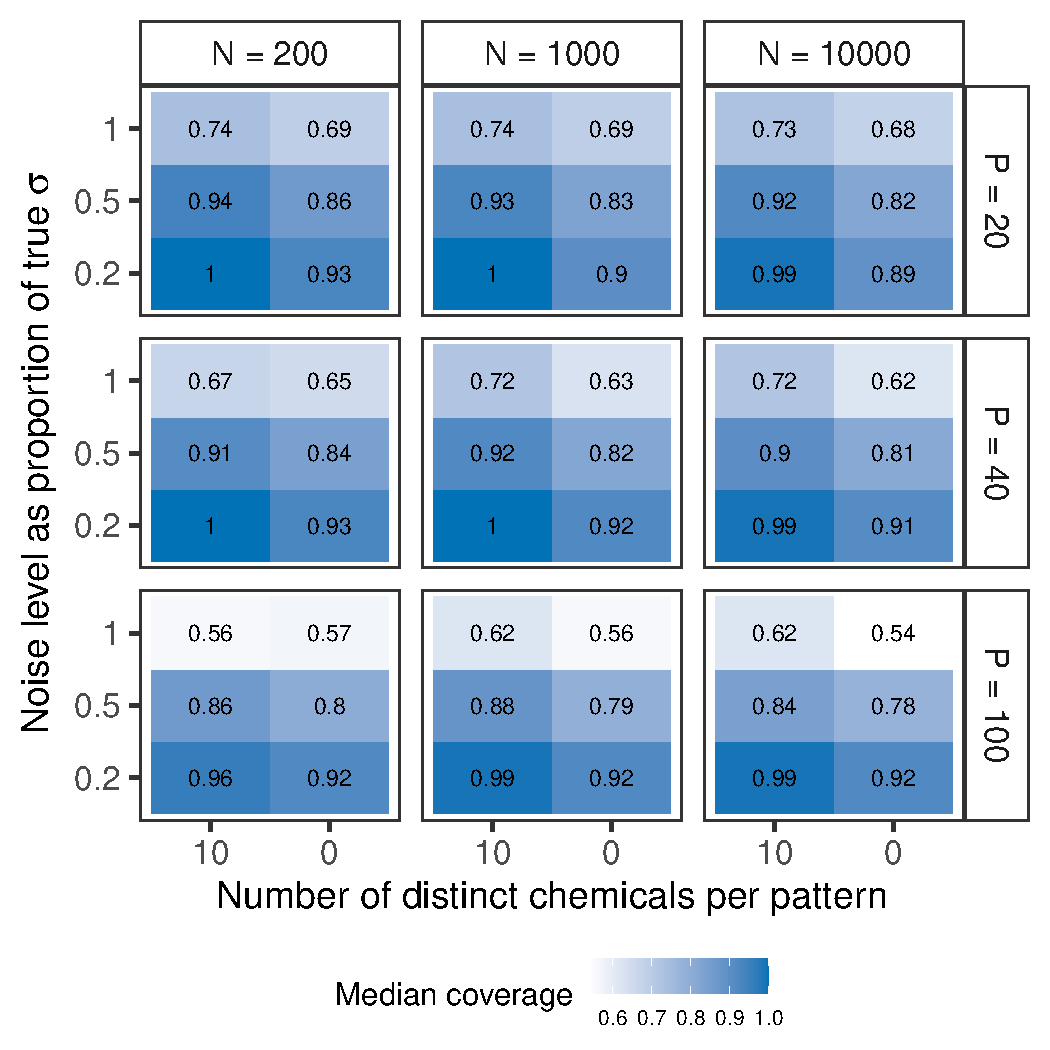
\includegraphics[scale = 0.8]{./figures/coverage_dim_np.pdf}
\end{figure}

\begin{figure}[!htbp]
\caption[Variational coverage for secondary simulations across rank]{Ninety-five percent variational confidence interval coverage across simulations with different values of $K$. Squares are colored according to median coverage (proportion of true values within estimated 95\% variational confidence intervals). Median was taken across all solutions that estimated the correct number of patterns for all combinations of $N$ = 200, 1,000, and 10,000 and $P$ = 20, 40, and 100. On the x axis, number of distinct chemicals per pattern is 10 (distinct) or 0 (overlapping). On the y axis, added noise level relative to the true standard deviation increases from 0.2 (low added noise) to 1 (as much added noise as true noise). Each panel describes simulations of a different rank, with each column representing a different number of patterns. Gray squares indicate that \bnmf never estimated the correct pattern number.}
\label{fig:pattern_coverage}
\centering
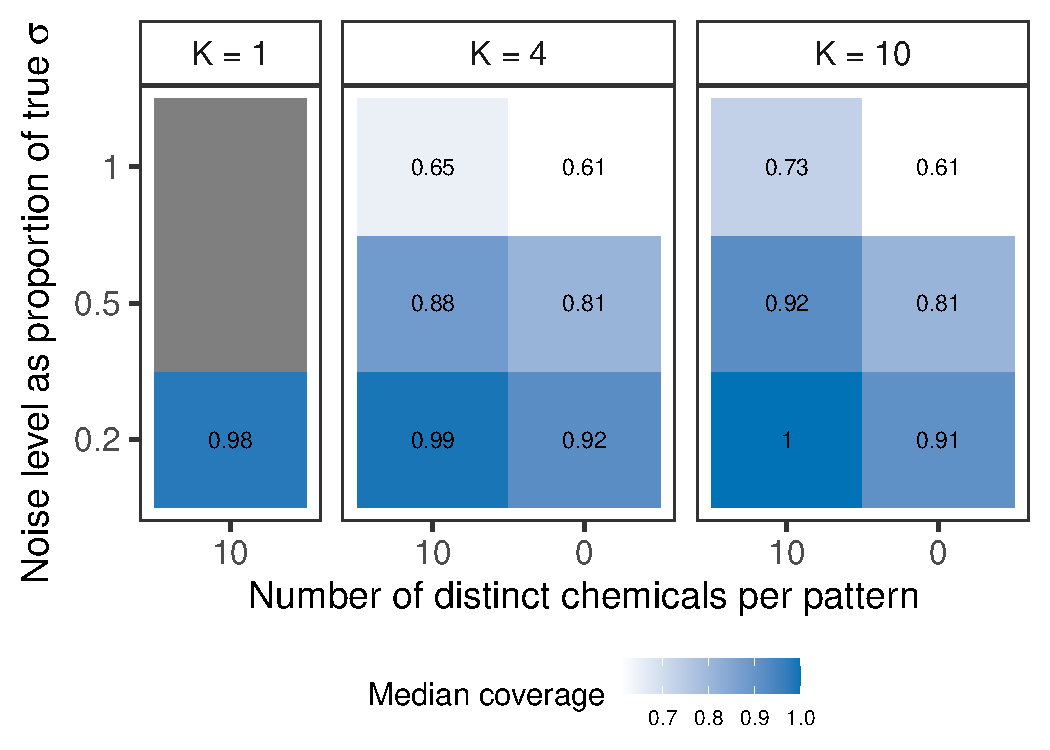
\includegraphics[scale = 0.8]{./figures/coverage_dim_k.pdf}
\end{figure}
} % put supplemental numbering in curly braces

\chapter[Prenatal endocrine disrupting chemical exposure \& child IQ]{Prenatal endocrine disrupting chemical exposure \& child IQ: {\LARGE Accounting for uncertainty in pattern identification in a two-stage health analysis}}\label{sec:ch4}
\vspace{-3em}

\begin{center}
Elizabeth A. Gibson,\textsuperscript{1} 
Robbie M. Parks,\textsuperscript{1}
Pam Factor-Litvak,\textsuperscript{2} 
Jeff Goldsmith,\textsuperscript{3} 
John Paisley,\textsuperscript{4} 
Julie B. Herbstman,\textsuperscript{1} 
Marianthi-Anna Kioumourtzoglou\textsuperscript{1} \\ 

\textbf{Affiliations:} \\ 1. Department of Environmental Health Sciences, Columbia University; \\ 
2. Department of Epidemiology, Columbia University; \\ 
3. Department of Biostatistics, Columbia University; \\ 
4. Department of Electrical Engineering, Columbia University. 
\end{center}

\clearpage

%% main text
\section{Introduction}
The prevalence of neurodevelopmental disorders in the U.S. has increased over previous decades \cite{boyle2011trends}. Even a small downward shift may have a substantial population impact \cite{gore2015edc}. In a large population, a five-point reduction in intelligence quotient (IQ) results in a doubling in the absolute number of individuals with IQ scores consistent with intellectual disabilities (IQ $<$ 70) \cite{braun2017early}, which has further downstream consequences for reduced societal productivity and economic loss \cite{bellanger2015neurobehavioral}. To inform the design of strategies promoting neurological health, we must identify modifiable risk factors, such as environmental contributors, including EDCs endocrine disrupting chemicals (EDCs) \cite{sathyanarayana2008phthalates, gore2015edc}. EDCs, such as phenols and phthalates, specifically, appear as plasticizers, preservatives, and additives in a wide variety of personal care products and food packaging, making exposure ubiquitous \cite{philippat2015exposure, schettler2006human, lorber2015exposure, koniecki2011phthalates}. 

Phenols and phthalates are not chemically bound to products, causing human exposure through inhalation, absorption, and ingestion \cite{vandenberg2007human}, and both cross the placenta during pregnancy \cite{schonfelder2002parent, mose2007phthalate}. Mounting evidence connects EDC exposures, such as phthalates \cite{van2020phthalate, nidens2020prenatal, kim2018association, doherty2017prenatal, kim2011prenatal}, triclosan \cite{jackson2018identifying, guo2020early}, parabens \cite{freire2020association}, and bisphenol A (BPA) \cite{jiang2020prenatal, lin2017prenatal}, during the critical \textit{in utero} period with adverse child cognitive development in childhood. Within the Columbia Center for Children’s Environmental Health's (CCCEH) Mothers and Newborns birth cohort, we have previously reported associations between prenatal exposure to individual phthalates and child cognitive development \cite{factor2014persistent, whyatt2012maternal}. Because associations between single EDCs and cognition do not encompass collective exposure to multiple chemicals simultaneously, interest in EDCs as an environmental mixture continues to increase \cite{braun2016can, taylor16}. Research has broadened to include joint and interactive effects among chemicals \cite{hu2021prenatal}, EDC mixture exposure profiles \cite{kalloo2021chemical}, and the overall effect of the EDC mixture \cite{tanner2020early}.

Here, we investigate a mixture of 17 phenols and phthalate metabolites measured in spot urine samples collected during the third trimester of pregnancy. To assess exposure to all EDCs simultaneously and to identify patterns within the mixture, we consider the high dimensionality of the exposure matrix and the complex correlation structures across the chemicals \cite{taylor16}. We propose a two-stage Bayesian model for estimating health effects of patterns of environmental exposures. In the first stage, we fit a non-parametric non-negative matrix factorization (\bnmfc) that performs pattern recognition within an environmental mixture, as described in Chapter~\ref{sec:ch3}; subsequently, we propagate the uncertainty from the first stage in a hierarchical regression model to estimate the association between exposure patterns and the health outcome. The primary goal of this research is to describe relationships between \bnmfc-identified patterns of \textit{in utero} EDC exposure (while properly incorporating our confidence in these patterns) and child cognition at seven years of age.

\section{Methods}

\subsection{Study Population}
For this study, we included a subset of mother-child dyads enrolled in the CCCEH Mothers and Newborns longitudinal birth cohort. This cohort study was initiated to evaluate the effects of prenatal exposure to air pollutants on birth outcomes and cognitive and behavioral development in children. A total of 727 African American and Dominican women were recruited from two prenatal clinics in Northern Manhattan between 1998 and 2006. Enrollment, exclusion criteria, and a description of the cohort have been described previously \cite{perera03}.

We included mothers in the current study if phthalate metabolite and phenol concentrations were measured in their spot urine samples collected during pregnancy (n = 343). We included all mothers with chemical measurements in the pattern identification step (see Section ~\ref{sec.patterns}). Children were selected for participation in the health analysis if their mothers were included in the pattern identification and if they completed the Wechsler Intelligence Scale for Children, 4th edition (WISC-IV) at age 7 years (n = 311). We saw no significant differences between these subsets and the overall Mothers and Newborns cohort in WISC-IV full scale IQ or covariates (see Supplemental Table~ref{table:suptable1}). Participating mothers provided written informed consent for themselves and their child, children provided their assent to participate beginning at age 7, and Columbia University Medical Center's Institutional Review Board approved the study procedures.

\subsubsection{Phthalate \& phenol measurements}
We collected spot urine samples during the third trimester of pregnancy. Eight environmental phenols (Benzophenone-3 (BP-3), triclosan, 2,4-dichlorophenol (24-DCP), 2,5- dichlorophenol (25-DCP), methyl paraben (M-PB), propyl paraben (P-PB), butyl paraben (B-PB), and bisphenol A (BPA)) and nine phthalate metabolites (Mono-2-ethylhexyl (MEHP), mono-2-ethyl-5-carboxypentyl (MECPP), mono-2-ethyl-5-hydroxyhexyl (MEHHP), mono-2-ethyl-5-oxohexyl (MEOHP), mono-benzyl (MBZP), mono-3-carboxypropyl (MCPP), mono-n-butyl (MBP), mono-isobutyl (MIBP) and mono-ethyl (MEP)) were measured at the U.S. Centers for Disease Control and Prevention (CDC) as described previously \cite{ye2005automated, calafat2008exposure, silva2004urinary}. The limits of detection (LODs) ranged from 0.2 to 2.3 ng/ml urine for phenols and 0.2 to 2.3 ng/ml urine for phthalates. Concentrations of phenols and phthalate metabolites were specific gravity-adjusted to account for urinary dilution \cite{hauser2004temporal}. These markers are non-persistent, and repeated measures have show inconsistency over time in other samples \cite{fisher2015bisphenol}. However, previous research in the Mothers and Newborns cohort showed moderate reliability over a short time span, approximating continuous exposure. Intra-class correlation coefficients were 0.77 for MBZP, 0.65 for MnBP, 0.60 for MIBP, and between 0.27 and 0.42 for the di(2-ethylhexyl) phthalate (DEHP) metabolites \cite{whyatt2012maternal, factor2014persistent}.

\subsubsection{Child intelligence measurement}
The WISC-IV was administered to children at age seven \cite{wechsler2003}. The WISC-IV full scale IQ represents a child's general intellectual performance across four indices: verbal comprehension, perceptual reasoning, working memory, and processing speed. The WISC-IV has been validated among both English- and Spanish-speaking populations and has been shown to be sensitive to low-dose exposure of certain individual phthalates and phenols \cite{factor2014persistent, guo2020prenatal}.

\subsubsection{Model covariates}
\label{sec:cov}
Extensive data were collected using medical records and questionnaires administered during pregnancy. Potential confounders included maternal age, intelligence, and education (less than high school vs. at least high school or equivalent), marital status (ever married vs. never married), and material hardship (any reported vs. none reported). Strong predictors of the outcome included alcohol use during pregnancy (any wine, beer, or liquor vs. none) and quality of the care-taking environment (measured at child age three). The quality of the home environment was measured by the Home Observation for Measurement of the Environment (HOME) scale \cite{caldwellhome}. Maternal intelligence was assessed by the Test of Non-Verbal Intelligence, third edition, a language-free measure of general intelligence \cite{brown1990test}. We scaled continuous covariates (maternal age, IQ, and HOME score) to mean zero and standard deviation one. Seven percent of eligible children were excluded (n=22 of N=311) due to missing covariate data. We examined the data for patterns between variables with missing values and others using a Kruskal-Wallis test to compare with continuous variables and a chi-squared test for discrete variables. We confirmed that missingness did not relate to any other data in the dataset, i.e., variables were missing completely at random (MCAR).

\subsection{Statistical analysis}
We examined distributional plots and descriptive statistics for all variables. We assigned phthalate metabolite and phenol concentrations below the limit of detection (LOD) the value of $LOD/\sqrt{2}$ \cite{hornung1990estimation}. We scaled all concentrations to standard deviation equal to 1 prior to the pattern identification step. Analyses were conducted using R version 4.0.4 and Stan version 2.26 \cite{rrr, gelman2015stan}. 

\subsubsection{Pattern identification}
\label{sec.patterns}
\bnmf is a pattern recognition tool which reduces the dimensionality of a chemical mixture, expressing individual exposure in terms of their underlying patterns (see Chapter~\ref{sec:ch3} for more details). \bnmfc-identified individual scores and chemical loadings are similar to frequentist non-negative matrix factorization (NMF) in their interpretation. Non-negativity puts the results on the same range as the original chemical concentrations and provides solutions interpretable on an additive scale with a parts-based representation \cite{holtzman2018machine, lee1999learning}. \bnmf is distinct from traditional NMF in two important ways. First, the Bayesian framework allows for uncertainty in estimation. This is expressed as a distribution around individual scores and chemical loadings on patterns. In this work, we incorporated the distributions around individual point estimates as hierarchical exposures in the health model (see Section~\ref{sec.health}), which included our confidence in the pattern recognition step in the 95\% credible intervals around $\beta$ coefficients. \bnmfc's non-parametric prior on the number of patterns in a mixture also distinguishes it from other NMF methods, which require an \textit{a priori} specification or \textit{post-hoc} selection of pattern number. \bnmf helps to remove the researcher from specification and selection of pattern number, estimating it from the data. Here, we used individual scores on \bnmfc-identified patterns across 17 phthalates and phenols measured in pregnant women from a previous analysis described in Section~\ref{results_app}.

For a matrix $X =\lbrace x_{i j}\rbrace $ of $i = 1:N$ individuals and $j = 1:P$ chemicals, \bnmf identifies matrices $W$ and $H$ and the vector $\mathbf{a}$ arising from the following data generating process,
\begin{equation}
\label{nmf}
X_{i j} \sim \operatorname{Poisson}\left(\sum^K_{k=1} W_{i k} \mathbf{a}_k H_{k j}\right)
\end{equation}

Where $K$ is the number of patterns determined by the model. $W$, $H$, and $\mathbf{a}$ all have Gamma priors; the Gamma distribution is over non-negative real numbers, so this enforces non-negativity on the solution. The vector $\mathbf{a}$ has a sparse Gamma prior to optimally shrink the number of patterns. We obtained individual scores from the posterior distribution, ${W\operatorname{diag}(\mathbf{a}) \sim \operatorname{Gamma}(\alpha_W, \beta_W)} \times
\operatorname{Gamma}(\alpha_\mathbf{a}, \beta_\mathbf{a})$. The expectation of this distribution, $\mathbb{E}[\widehat{W}\operatorname{diag}(\widehat{\mathbf{a}})]$, represents individuals' exposure concentrations on the $K$ identified patterns. We also obtained chemicals loadings from the posterior distribution, $H \sim \operatorname{Gamma}(\alpha_H, \beta_H)$. The expectation, $\mathbb{E}[\widehat{H}]$, defines each pattern's unique mixture of chemical loadings.

To standardize values from \bnmfc, we normalized chemical loadings over patterns (i.e., divided each loading by the sum of all loadings on a pattern) and multiplied individual scores by their corresponding normalization constant. This put individual scores on different patterns on the same scale. We further transformed patterns to have standard deviation equal to one across individual scores to enable interpretation of the coefficient size in the subsequent regression model as corresponding to a one standard deviation increase in the exposure pattern.

\subsubsection{Health models}
\label{sec.health}
\paragraph{Traditional models.} We conducted multivariable linear regression analyses to evaluate the relationships between prenatal EDC exposure patterns and continuous full scale IQ scores. We refer to these models as `traditional' throughout this work because environmental health and epidemiological research has traditionally worked within a frequentist framework. We ran pattern-specific models for $\mathbb{E}[\widehat{W}_1\widehat{\mathbf{a}}_1]$ and $\mathbb{E}[\widehat{W}_2\widehat{\mathbf{a}}_2]$, adjusting for covariates, because identified patterns were not correlated ($r$ = -0.07). We place `hats' on these quantities to emphasize that they were estimated by \bnmf in the first stage of our analysis. Final regression models included covariates that were \textit{a priori} defined as potential confounders based on previous literature and a directed acyclic graph, or that were strong predictors of full scale IQ (see Section~\ref{sec:cov}) \cite{pearl2009causality, hernan2010causal}. We used penalized splines to investigate deviations from linearity and determined that linear models fit the data well. Because there is a large body of evidence indicating sex-specific associations between endocrine disrupting chemicals and health outcomes, we included sex as an effect modifier in all models and present sex-specific results.

We identified influential outliers using Studentized residuals, which scale each residual by its corresponding standard deviation, and Cook's distance, which measures the effect of deleting a given observation on the remaining data \cite{kleinbaum2013applied}. Two observations with values $>$ 5 standard deviations from  the phthalate + BPA pattern mean were identified and removed for the main analysis.

\paragraph{Bayesian hierarchical models.} Because our traditional regression models did not account for the inherit uncertainty in the first stage of this analysis, we next fit Bayesian health models. This allowed us to incorporate the distributional information from \bnmf in the regressions. \bnmf generated individual scores from the product of two Gamma distributions, $\widehat{W}$ and $\widehat{\mathbf{a}}$, and we used these distributions to build a hierarchical likelihood as follows,
\begin{equation}
\begin{aligned}
Z_i & \sim \operatorname{Gamma}(\widehat{\alpha}_{W i}, \widehat{\beta}_{W i}) 
    \times \operatorname{Gamma}(\widehat{\alpha}_{\mathbf{a} i},
    \widehat{\beta}_{\mathbf{a} i})  \\
Y_i & = \beta_0 + \beta_Z Z_i + \beta_{S} S_i 
+ \beta_{Z \cdot S} \left(Z_i S_i\right) 
+ \mathbf{X}_{i}^T\boldsymbol{\beta}_\mathbf{X} + \varepsilon_i \\
\end{aligned}
\end{equation}

For $i = 1 ... N$, $Z_i$ is the individual pattern score drawn from the distribution estimated by \bnmfc, with scale and rate parameters $\widehat{\alpha}_{W i}$ and $\widehat{\beta}_{W i}$ for the distribution over $\widehat{W}_i$ and $\widehat{\alpha}_{\mathbf{a} i}$ and $\widehat{\beta}_{\mathbf{a} i}$ for the distribution over $\widehat{\mathbf{a}}_i$. The outcome $Y_i$ is continuous full-scale IQ; $\beta_0$ is the intercept;  $S_i$ is child's sex; $Z_i S_i$ is the interaction term between individual pattern score and sex; and $\mathbf{X}_{i}$ is a vector of additional covariates. The regression coefficients \(\beta_Z\), \(\beta_S\), \(\beta_{Z \cdot S}\), and \(\beta_\mathbf{X}\) relate their subscript to the outcome, and $\varepsilon_i$ is residual error.

We left improper, non-informative priors on $\beta$'s and $\varepsilon$, putting equal weight on all real numbers for $\beta$ coefficients, \(\mathbb R \), and over all non-negative real numbers, \(\mathbb R_{\geq 0}^+\), for the intercept ($\beta_0$) and the standard deviation of the error term ($\varepsilon \sim \mathcal{N}(0,\sigma^2)$). These priors are improper in that they did not integrate to one (though the posterior does) and non-informative in that they were dominated by the data and played a minimal role in the posterior distribution. This made the results more comparable to those from our traditional regression.

\subsubsection{Sensitivity analyses}
We performed two sensitivity analyses: 1) we evaluated the influence of prior specification for the Bayesian health models by fitting models with alternative priors (weakly informative and a weak/non-informative hybrid) allowing for different assumptions and the incorporation of prior knowledge (see Supplemental Materials Section~\ref{sec:priors}; and 2) we reran all analyses on the full dataset including outlying values.

\section{Results}
\subsection{Study sample characteristics}

We present summary statistics for maternal demographic characteristics, child sex (recorded at birth), and IQ at age seven in Table~\ref{tab:1}. The 311 study subjects did not differ significantly from the overall CCCEH cohort in terms of demographics (race/ethnicity, maternal marital status, maternal age, maternal education level), material hardship, prenatal alcohol consumption, presence of a smoker in the home, quality of the home environment, child sex, or child IQ. \\

\begingroup
\renewcommand{\arraystretch}{1.4}
\begin{table}[!ht] \centering 
\caption[Subject demographics in Mothers and Newborns cohort]{Subject demographics and distribution of potential confounders, model covariates, and outcome variable (N = 311).}
  \label{tab:1} 
  \addtolength{\tabcolsep}{-2pt}
\begin{tabular}{l|rr}
Characteristic & \multicolumn{2}{c}{Value\textsuperscript{*}} \\
\hline 
\hline
Ethnicity & \\
\hline
\hspace{1em}African American & 107 & 34.4 \\
\hline
\hspace{1em}Hispanic/Latina & 204 & 65.6 \\
\hline
Maternal education & \\
\hline
\hspace{1em} $\le$ High school degree or equivalent & 196 & 63.0 \\
\hline
\hspace{1em} $<$ High school degree & 115 & 37.0 \\
\hline
Material hardship & 128 & 41.2 \\
\hline
Marital status & \\
\hline
\hspace{1em}Never Married & 209 & 67.2 \\
\hline
\hspace{1em}Ever Married & 102 & 32.8 \\
\hline
Prenatal alcohol consumption & 77 & 24.8 \\
\hline
Smoker in home & 94 & 30.2 \\
\hline
Child sex & \\
\hline
\hspace{1em}Male & 166 & 53.4 \\
\hline
\hspace{1em}Female & 145 & 46.6 \\
\hline
Maternal age at delivery & 25.5 & 4.9 \\
\hline
Maternal IQ & 84.9 & 13.4 \\
\hline
HOME scale & 39.3 & 6.3 \\
\hline
Child Full Scale IQ & 97.3 & 13.3 \\
\hline 
\hline
%\vspace{1ex}
\multicolumn{3}{l}{\textsuperscript{*} n, \%; Mean, SD} 
\end{tabular}
\end{table}
\endgroup 

Table~\ref{tab:conc} describes the distributions of phenol and phthalate metabolite concentrations measured in maternal spot urine samples. Fourteen phenols and phthalate metabolites were detected in 93\%--100\% of samples; the exceptions were BPB (38\% $<$ LOD), triclosan (20\% $<$ LOD), and MEHP (16\% $<$ LOD). We depict Spearman correlations ($r_S$) between specific-gravity adjusted phenols and phthalate metabolites in Figure~\ref{fig:corr}. Phthalate metabolites were generally positively correlated. Four metabolites of DEHP had correlations ($>$ 0.7). Within phenols, 24-DCP and 25-DCP ($r_S$ = 0.94) and PPB and MPB ($r_S$ = 0.75) showed the highest correlations. MEP was notably correlated with two phenols ($r_S$ = 0.42 with PPB, and $r$ = 0.44 with MPB), which appeared in the \bnmf solution. \\

\begingroup
\renewcommand{\arraystretch}{1.25}
\begin{table}[!ht] \centering 
  \caption[Distribution of phthalate metabolites and phenols]{Distribution of phthalate metabolites and phenols (ng/ml) in maternal spot urine and distribution of \bnmfc-identified patterns in the overall mixture during the third trimester of pregnancy (n = 343).}
  \label{tab:conc} 
\begin{tabular}{@{\extracolsep{5pt}} llrrrr} 
Class & Chemical & \% \textless LOD & 25\% & Median & 75\% \\ 
\hline 
\\[-3ex] \hline \\[-2.5ex]
\multirow{8}{*}{Phenols} & BPB    & 38.5 & 0.2  & 0.4 & 2.0 \\ 
& BP-3   & 0.6 & 4.8  & 8.9 & 26.3 \\ 
& BPA    & 6.7 & 1.1  & 1.8 & 3.2 \\ 
& 24-DCP & 0.6 & 1.6  & 3.0 & 6.0 \\ 
& 25-DCP & 0.0 & 38.0 & 81.8 & 205.6 \\ 
& MPB    & 0.0 & 46.1 & 132.4 & 363.7 \\ 
& PPB    & 0.0 & 5.3  & 20.4 & 71.9 \\ 
& TCS    & 20.0 & 3.5  & 8.7 & 36.7 \\ 
\hline
\multirow{9}{*}{Phthalates} & MBP    & 0.0 & 22.8 & 37.1 & 66.4 \\ 
& MBZP   & 0.0 & 6.6  & 13.0 & 27.4 \\ 
& MCPP   & 4.4 & 1.4  & 2.3 & 3.7 \\ 
& MECPP  & 0.0 & 21.0 & 35.4 & 69.0 \\ 
& MEHHP  & 0.0 & 11.3 & 21.0 & 40.0 \\ 
& MEHP   & 15.7 & 2.3  & 4.9 & 11.5 \\ 
& MEOHP  & 0.0 & 9.8  & 17.1 & 32.5 \\ 
& MEP    & 0.0 & 77.6 & 143.6 & 333.7 \\ 
& MIBP   & 0.6 & 5.5  & 9.6 & 16.1 \\ 
\hline 
 & Phthalates + BPA & --- & 2.8 & 4.2 & 6.1 \\
 & Phenols + MEP & --- & 2.2 & 3.4 & 6.9 \\
\hline
\\[-3ex] \hline \\[-2.5ex]
\end{tabular} 
\end{table} 
\endgroup

\subsection{Pattern recognition}
\bnmfc-identified patterns were described in detail in Section~\ref{results_app} and are presented again in Figure~\ref{fig:load}. Briefly, we found two prominent patterns within the EDC mixture, one phenol pattern and one phthalate pattern, with notable cross-class loadings: MEP loaded more strongly onto the pattern described by phenol exposure (we will refer to this pattern as phenols + MEP), and BPA loaded more strongly on the pattern comprised of phthalate metabolites (we will refer to this pattern as phthalates + MEP). While these chemicals appear in various consumer products, these patterns appear to reflect distinct exposure routes, phenols + MEP through personal care products and phthalates + BPA through food packaging. Patterns were not correlated ($r_S$ = -0.07). Summary statistics for the two patterns are presented in Table~\ref{tab:conc}.

\subsection{Traditional health models}
Table~\ref{tab:reg} displays associations between prenatal exposure to \bnmfc-identified EDC patterns and child IQ in males and females from multivariable linear regression models. In these traditional regression models, we used the mean of each individual score distribution as a point estimate to assign pattern exposure. Adjusting for coviarates, full scale IQ was, on average, negatively associated with phthalate + BPA exposure in females ($\beta$ = -3.4; 95\% confidence interval (CI) = -6.5, -0.4) but not in males ($\beta$ = -0.4; 95\% CI = -2.4, 1.7). The interaction term between males and females was marginally significant (p-value $<$ 0.1). Phenols + MEP were not associated with full scale IQ in males ($\beta$ = -0.8; 95\% CI =  -2.7, 1.1), but there was suggestive evidence of a positive association in females ($\beta$ = 2.0; 95\% CI = -0.3, 4.2). The interaction term between males and females was, again, marginally significant (p-value $<$ 0.1).

\begin{landscape}
\begin{figure}
\centering
\begin{subfigure}[b]{0.7\textwidth}
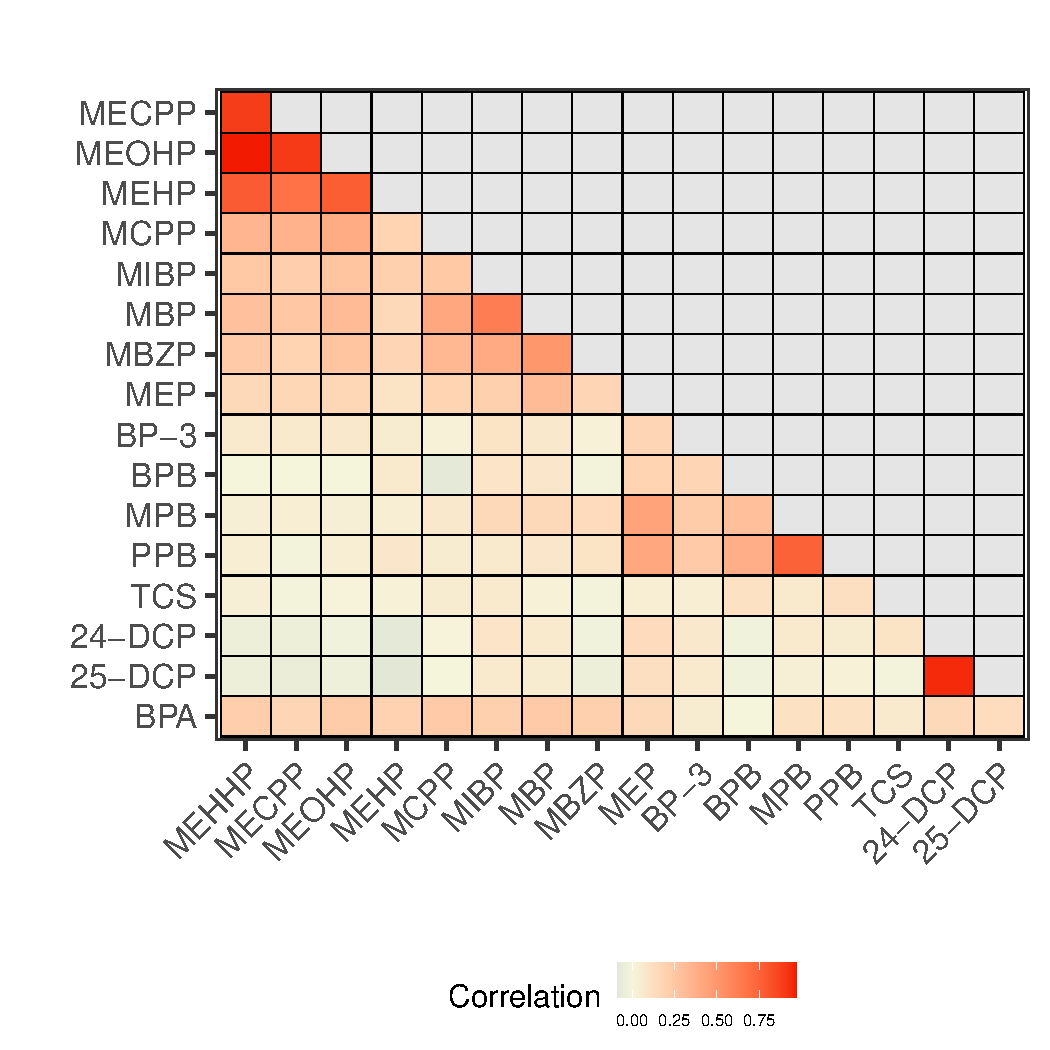
\includegraphics[scale = 0.69]{./figures/ppp_corr.pdf}
\caption{Inter-chemical correlations}
\label{fig:corr}
\end{subfigure}
\hspace{5em}
\begin{subfigure}[b]{0.3\textwidth}
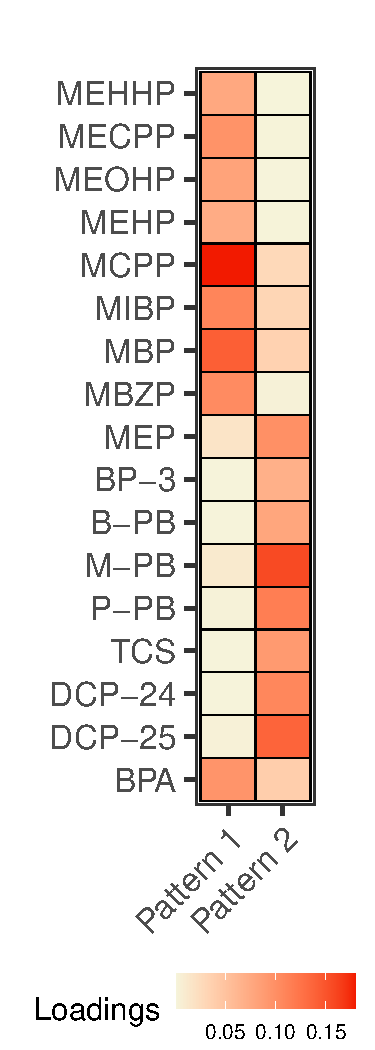
\includegraphics[scale = 0.69]{./figures/eh_loadings.pdf}
\caption{\bnmfc-identified loadings}
\label{fig:load}
\end{subfigure}
\hfill
\caption[Intra-chemical correlations and \bnmfc-identified chemical loadings]{(\textbf{a}) Spearman correlations between 17 specific gravity-adjusted endocrine disrupting chemicals measured in 343 pregnant women from the Mothers \& Newborns cohort. (\textbf{b}) \bnmfc-identified chemical loadings. \bnmf discovered two underlying patterns in the mixture of seventeen phenols and phthalate metabolites in pregnant women. One pattern was characterized by phthalates and BPA, the other by phenols and MEP.}
\end{figure}
\end{landscape}

\subsection{Bayesian health models}
Adjusting for covariates, full scale IQ was, on average, negatively associated with phthalate + BPA exposure in females ($\beta$ = -3.4; 95\% credible interval (CrI) = -6.7, -0.4) but not in males ($\beta$ = -0.4; 95\% CrI = -2.5, 1.7). Phenols + MEP were not associated with full scale IQ in females ($\beta$ = 2.1; 95\% CrI = -0.3, 4.5) or males ($\beta$ = -0.8; 95\% CrI = -2.8, 1.1). \\

\subsection{Sensitivity Analyses}
\subsubsection{Alternative prior distributions}
Altering the prior structure had no effect on inference. $\beta$ coefficients were, in general, unaffected or slightly farther from the null with weakly informative priors and in the hybrid scenario, and 95\% credible intervals were generally unaffected or slightly wider. As in the main analysis, full scale IQ was, on average, negatively associated with phthalates + BPA exposure in females but not in males. Phenols + MEP had no association with child intelligence. Results from Bayesian hierarchical regression models with differently-specified priors are available in Supplemental Table~\ref{tab:supreg}.

\begingroup
\renewcommand{\arraystretch}{1.25}
\begin{table}[!ht] \centering 
  \caption[Multivariable regression models of WISC-IV full scale IQ]{Results from multivariable regression models of WISC-IV full scale IQ at age seven.} 
  \label{tab:reg} 
\begin{tabular}{llrcrc} 
& & \multicolumn{2}{c}{\textit{Traditional model\textsuperscript{*}}} & \multicolumn{2}{c}{\textit{Bayesian model\textsuperscript{*}}} \\
\hline 
\\[-3ex] \hline
 & Term & $\beta$ & 95\% CI\textsuperscript{$\dagger$} & $\beta$ & 95\% CrI\textsuperscript{$\dagger$} \\ 
\hline 
\\[-3ex] \hline
\multirow{3}{*}{Phthalates + BPA} & Females & -3.4  & (-6.5, -0.4) &  -3.4 & (-6.7, -0.4) \\ 
                           & Males & -0.4 & (-2.4, 1.7)   &  -0.4 & (-2.5, 1.7) \\ 
                           & Interaction term & -3.1 & (-6.7, 0.6)   &  -3.0 & (-6.9, 0.6) \\ 
\hline
\multirow{3}{*}{Phenols + MEP} & Females          & 2.0   & (-0.3, 4.2) & 2.1 & (-0.3, 4.5) \\ 
                           & Males            & -0.8  & (-2.7, 1.1) & -0.8 & (-2.8, 1.1) \\ 
                           & Interaction term & 2.8   & (-0.2, 5.8) & 2.9 & (-0.1, 6.0) \\ 
\hline 
\\[-3ex] \hline \\[-2.5ex]
%\multicolumn{2}{l}{\rule{0pt}{1em}\textsuperscript{*} $p < 0.05$}\\
\multicolumn{6}{p{0.85\linewidth}}{\textsuperscript{*} Models adjusted for maternal age, IQ, and education, prenatal alcohol consumption, marital status, HOME score, and material hardship.} \\
\multicolumn{6}{p{0.85\linewidth}}{\textsuperscript{$\dagger$} 95\% CI = confidence interval for traditional regression, CrI = credible interval for Bayesian regression.} \\
\end{tabular} 
\end{table} 
\endgroup

\subsubsection{Assessing effects of outlying values}
We reran multivariable regression models with the full data. We found significant deviation from linearity with the retention of these observations, which diverged from the trend in the main analysis. Supplemental Figure~\ref{fig:fulldat} contrasts our findings with the sensitivity analysis.

\section{Discussion}
% Quick recap findings
In this work, we used \bnmf to identify patterns of phenols and phthalate metabolites measured in spot urine samples from pregnant women. We saw a significant negative association between phthalates + BPA, which represented joint exposure to DEHP, di-n-butyl phthalate [DnBP], di-isobutyl phthalate [DiBP], benzylbutyl phthalate [BzBP], and BPA, and WISC-IV full scale IQ in female children at age seven. We observed no associations with phenols + MEP. We found suggestive evidence of sex-specific associations between both patterns and child IQ, though interaction terms did not reach statistical significance. Using a hierarchical Bayesian framework to incorporate the variability inherent in the pattern recognition step into the regression model, our inferences did not change. For both patterns, the direction and magnitude of the Bayesian $\beta$ coefficients matched those of the traditional models. Further, the Bayesian credible intervals, while not consistently wider, included the uncertainty of \bnmf in their coverage. This reinforces the findings of the traditional model. In quantifying the risk of cognitive deficits from EDCs---pervasive chemicals to which exposure may be preventable---we identified dietary sources of phthalates and BPA as a factor amenable to public health interventions, policy changes, or regulation.

% Continue here with summary of previous cohort results...
Our work builds on previous findings relating \textit{in utero} exposure to individual phthalates with sex-specific reductions in average child IQ in the Mothers and Newborns cohort \cite{factor2014persistent, whyatt2012maternal}. \citet{whyatt2012maternal} found negative associations between DnBP and mental development measured by the Bayley Scales of Infant Development (BSID), on average, in females at age three. \citet{factor2014persistent} extended these findings, identifying negative associations between DnBP and DiBP and average WISC-IV full scale IQ in children at age seven. DnBP and DiBP, notably, loaded strongly with phthalates + BPA in our analysis. Prenatal phthalate exposure in these children has also been linked to other developmental outcomes such as visual recognition memory \cite{ipapo2017maternal}, motor skills \cite{balalian2019prenatal, daniel2020perinatal}, and behavioral problems \cite{daniel2020prenatal}.

% Wider single chem results 
Many research groups have examined the relationship between \textit{in utero} phthalate exposure and child cognition. In another New York City cohort, \citet{engel2009prenatal} found associations between high molecular weight phthalate metabolites in pregnant women and neonatal behavior. In the same cohort, \citet{doherty2017prenatal} found lower average mental development among female children prenatally exposed to DnBP. \citet{jankowska2019phthalate} found negative associations between DnBP and dimethyl phthalate and general intellectual ability in seven year old Polish children. In a Mexican cohort, \citet{tellez2013prenatal} found a negative association between DEHP exposure and average mental development in female children between two and three years of age. In a U.S. cohort, \citet{li2019identifying} found a negative association between monobenzyl phthalate exposure at 16 weeks gestation and average full scale IQ at ages five and eight. These studies, notably, all evaluated multiple phthalates assessed individually (rather than as part of a mixture), and all reported null associations between some phthalates and child cognition \cite{radke2020phthalate}. Further inconsistency exists, as some researchers reported only null results \cite{hyland2019prenatal, nakiwala2018utero} or associations in males but not in females \cite{zhu2020domain, torres2020early, kim2011prenatal}. Variability in results may be due to a number of factors, such as timing of phthalate measurements during pregnancy, age of cognitive assessment in the children, cognitive tests measuring different constructs (e.g., WISC-IV vs. BSID), insufficient adjustment for confounders (potentially including other phthalate metabolites), varying phthalate concentrations in study populations, or differences in the distributions of distinct effect modifiers in the study population. 

\bnmf also identified a second pattern representing phenols and MEP that was not associated with child IQ. However, previous 
research has shown association between individual phenols and child cognition. In a U.S. cohort, \citet{jackson2018identifying} found maternal urinary triclosan concentrations at delivery were associated with lower cognitive test scores, on average, in eight year old children of both sexes. \citet{freire2020association} found placental concentrations of PPB were associated with poorer memory and motor function, on average, in Spanish children between four and five years of age.

% other mixtures results
Because individuals are not exposed to phenols or phthalates in isolation, research increasingly aims to account for simultaneous exposures to these chemicals as environmental mixtures. Within this area of research, different statistical methods have been employed to answer different questions \cite{gibson2019complex}. For example, weighted quantile sum (WQS) regression has been used to answer research questions concerning the overall effect of an EDC mixture on child cognition and the identification of potential chemicals of concern \citet{tanner2020early, loftus2021exposure}.

Beginning with a research question more similar to our own, \citet{kalloo2021chemical} used k-means clustering, a traditional pattern recognition tool, to identify pregnant women with similar chemical exposure profiles within a mixture of EDCs (including phenols and phthalates), metals, and environmental tobacco smoke. In a two-stage analysis, they found that children born to women in the k-means-identified `cluster 1' had lower scores on the performance IQ subscale compared with the reference cluster. Membership in `cluster 1' indicated higher concentrations of DEHP metabolites, MBP, BPA, triclosan, and BP-3, among others, and lower exposure to parabens, MBZP, MIBP, and MEP. While our results are not directly comparable, both studies identified relationships between patterns or profiles expressing exposure to DEHP metabolites and BPA and child IQ, though \citet{kalloo2021chemical} found no evidence of sex-specific associations.

% what's cool about \bnmf
We originally adapted \bnmf to environmental epidemiology to address specific impediments to pattern recognition in environmental mixtures. First, we cannot know the true underlying number of patterns. To reduce the need for \textit{post hoc} pattern selection and foster reproducibility of analyses, \bnmf includes an empirical sparse prior to choose the number of patterns in the mixture. Second, epidemiologists and environmental heath scientists generally desire interpretable patterns, as opposed to solely dimension reduction. \bnmfc's non-negative priors return results on an additive scale that encourages interpretability \cite{lee1999learning}. Finally, as in this analysis, pattern recognition in environmental health is often followed by a health model to estimate relationships between patterns and outcomes. Traditional methods ignore any uncertainty in pattern identification. \bnmf provides score distributions that can propagate uncertainty into health models.

% limitations
Our findings should be interpreted in light of several limitations. First, as is the case when using chemical biomarkers, our study is susceptible to exposure measurement error, which may have biased our estimates towards the null. Second, some components may be metabolized faster than others, and our mixture includes measurements from both parent compounds and metabolites. If components with shorter half-lives are more toxic and their levels are not adequately captured in the single sample provided by the participants, this could impact both the \bnmf solution and the subsequent health effect estimates. Repeat measurements have shown that these markers fail to reliably approximate continuous exposure \cite{fisher2015bisphenol, braun2012variability}. However, previous research in the Mothers and Newborns cohort showed moderate to high intra-class correlation coefficients, indicating consistency over time \cite{whyatt2012maternal, factor2014persistent}. Third, our findings may not be generalizable to a more general population; our cohort is composed of low-income Dominican and African American mothers living in an urban environment, and the \bnmfc-identified EDC patterns may represent sources or behaviors distinct to this group. Fourth, Bayesian models, in general, are powerful in their ability to combine information from multiple sources (i.e., data and prior information), but when initial assumptions are wrong, the conclusions will be as well. We evaluated our models with posterior predictive checks and used both noninformative and weakly informative priors in an ongoing process of feedback and quality control. Fifth, our dataset is high-dimensional, with a large number of correlated chemical measurements for each participant. In this situation, \bnmf performs exceptionally, as it was first designed for geothermal spectrograms, sensor measurements of frequencies over time, which are at a finer resolution and higher dimension than our current problem domain \cite{holtzman2018machine}. Finally, though we adjusted for multiple factors that varied across households to account for potential confounding, we cannot exclude the possibility of residual confounding.

Our study has a number of strengths. First, the prospective cohort design ensures the temporal ordering of exposure and outcome. Second, all phenols and phthalate metabolites were measured at the CDC; their quality assurance/quality control reduces the possibility of bias in measurement. Third, the WISC-IV test has measured reliability and validity and is sensitive to effects of low-dose neurotoxicant exposures on cognition \cite{rauh2011seven, jusko2008blood, wechsler2003}. Finally, our statistical methods appropriately address our research question concerning the relationship between patterns of prenatal EDC exposure and child cognition. \bnmf incorporates joint exposures in identified patterns, which better reflects the entire EDC milieu than individual measurements. Our two-stage hierarchical Bayesian health model propagates the uncertainty from \bnmf in the subsequent regression model, providing robust results and improving inference.

\section{Conclusion}

Our analysis identified two patterns of phenol and phthalate exposure in pregnant women. One pattern grouped metabolites of several phthalates and BPA, which are commonly found in food containers and packaging; the other grouped the remaining phenols, including parabens and triclosan, with the metabolite of DEP, all of which are more prevalent in personal care products. We detected a significant association between phthalates + BPA and average full scale IQ in females, but not males, at age seven. These results add to a body of evidence that, though somewhat 
inconsistent, indicates harmful and often sex-specific effects of EDCs in child development. By measuring prenatal patterns of EDCs, we identified an exposure source resembling food packaging as a potential risk factor most amenable to policy changes or regulation.

\clearpage
{\setcounter{figure}{0} % put supplemental numbering in curly braces
\setcounter{table}{0}
\renewcommand{\thefigure}{4.S.\arabic{figure}}
\renewcommand{\thetable}{4.S.\arabic{table}}
\section{Supplemental Materials}

\subsection{Alternative prior distributions}
\label{sec:priors}
Noninformative prior specifications on the Bayesian model made the resulting parameter estimates more comparable with our traditional model. In Bayesian statistics, however, `weakly' informative priors are generally preferred because noninformative priors place a large portion of their probability mass on unreasonable parameters. In our example with child IQ as the outcome, a noninformative prior on $\beta$ implies that we believe a coefficient of $\pm$ 100 is as likely as a coefficient of zero, which is, of course, implausible. Weakly informative priors, on the other hand, contain enough information to regularize the posterior distribution (i.e., to keep it between relatively reasonable bounds), but they do not attempt to fully capture previous beliefs or to heavily weight scientific knowledge about underlying parameters \cite{bda3}. We set up two scenarios, one with weakly informative priors and the other with a combination of weakly informative and noninformative priors, as sensitivity analyses. These encoded information about parameters and we designed them so as not to overly influence the posterior. Our weakly informative priors were modeled after \citet{gelman2020regression}. We fit two alterative prior structures, (1) weakly informative, where the $\beta$ distribution for phthalates + BPA was based on previous results (explained below) and all other coefficients were centered at zero, and (2) weakly informative/noninformative hybrid, where the $\beta$ distribution for phthalates + BPA was based on previous results, the $\beta$ for phenols + MEP was distributed around zero, and all covariates kept noninformative priors. The two schemes included the same priors on $\alpha$, $\sigma$, and the $\beta$ coefficients of interest as follows,
\begin{align*}
& \alpha \sim \mathcal{N}(100, 45), 
& \sigma \sim \operatorname{Exponential}(\frac{1}{sd_y}), \\
& \beta_{PHT+BPA} \sim \mathcal{N}(-1.19, 2.5 \cdot sd_y), 
& \beta_{PHT+BPA \cdot s} \sim \mathcal{N}(-0.03, 2.5 \cdot sd_y), \\
& \beta_{PHN+MEP} \sim \mathcal{N}(0, 2.5 \cdot sd_y), 
& \beta_{PHN+MEP \cdot s} \sim \mathcal{N}(0, 2.5 \cdot sd_y)
\end{align*}

Here, $sd_y$ is the standard deviation of the observed full scale IQ. $\beta_{PHT+BPA}$ and $\beta_{PHN+MEP}$ are the coefficients for the phthalate + BPA pattern and the phenol + MEP pattern, respectively; $\beta_{PHT+BPA \cdot s}$ and $\beta_{PHN+MEP \cdot s}$ are the coefficients for the corresponding interaction terms with sex. The weakly informative and weakly/non- informative hybrid structures differed only in the prior distributions on covariates. In the first scenario, $\beta_{\ldots} \sim \mathcal{N}(0, 2.5 \cdot sd_y)$ to serve as a soft regularizers, where $\beta_{\cdots}$ includes the coefficients for sex and all covariates. In the second, priors on sex and other covariates were flat over $\beta_{\ldots} \sim \mathcal{U}(-\infty, \infty)$, so as not to affect inference. Because WISC-IV IQ scales are standardized to a mean of 100 and a standard deviation of 15 \cite{wechsler2003}, we modeled $\alpha$ as normally distributed around 100 with a wider standard deviation. The specified distributions and parameters for $\sigma$ and the $\beta$ coefficients also considered the scale of the outcome \cite{gelman2020regression}. The error in the model was drawn from an exponential distribution with rate $= \frac{1}{sd_y}$; this placed the bulk of the distribution below $sd_y$, with a long right tail to accommodate uncertainty. Weakly informative priors on $\beta$ coefficients for patterns and interaction terms were normally distributed. For phthalates + BPA, we used \citeauthor{factor2014persistent}'s results to determine our prior means. They estimated sex-specific individual associations between full scale IQ and five of the eight phthalate metabolites that loaded strongly with phthalates + BPA \cite{factor2014persistent}. We took the average coefficient size across the five reported in that paper in males as phthalates + BPA's prior mean. We took the average difference between coefficients in females and males as the prior mean of the interaction between phthalates + BPA and sex. We had no prior knowledge on the association between phenols + MEP and full scale IQ, so for phenols + MEP and the pattern's interaction term with and sex, we set the means to zero. For both patterns and both interaction terms, we set the standard deviation to $2.5 \cdot sd_y$ to make these priors only weakly informative. 

\clearpage
\begin{landscape}
\begingroup
\renewcommand{\arraystretch}{1.075}
\begin{table} \centering 
%\small
  \caption[Subject demographics in parent cohort and study population]{Subject demographics and distribution of potential confounders, model covariates, and outcome variable in full Mothers and Newborns cohort (N = 727), subsample with phenols and phthalates measured in urine (N = 343), subsample with full scale WISC-IV IQ measured at age 7 (N = 311), and subsamples with no missing covariates (N = 289).} 
  \label{tab:suptable1} 
\begin{tabular}{l|rr|rrr|rrr|rrr}
\hline
\hline
\multirow{2}{*}{Characteristic} & \multicolumn{2}{c}{Entire Cohort} & \multicolumn{3}{c}{\bnmf Subsample} & \multicolumn{3}{c}{WISC-IV Subsample} & \multicolumn{3}{c}{Complete Cases} \\
& \multicolumn{2}{c}{N = 727} & \multicolumn{3}{c}{N = 343} & \multicolumn{3}{c}{N = 311} & \multicolumn{3}{c}{N = 289} \\
\hline
 & \multicolumn{2}{c}{Value\textsuperscript{*}} & \multicolumn{2}{c}{Value\textsuperscript{*}} & P\textsuperscript{$\dagger$} & \multicolumn{2}{c}{Value\textsuperscript{*}} & P\textsuperscript{$\dagger$} & \multicolumn{2}{c}{Value\textsuperscript{*}} & P\textsuperscript{$\dagger$} \\
\hline
Ethnicity & & & & & $>$0.9 & & & 0.9 & & & $>$0.9 \\
\hspace{1em}African American & 254 & 34.9 & 119 & 34.7 & & 107 & 34.4 & & 100 & 34.6 & \\
\hspace{1em}Hispanic/Latina & 473 & 65.1 & 224 & 65.3 && 204 & 65.6 && 189 & 65.4 & \\
\hline
Maternal education & & & & & 0.8 & & & 0.8 & & & $>$0.9 \\
\hspace{1em}$\le$ High school degree or equivalent & 456 & 64.0 & 216 & 63.0 && 196 & 63.0 && 186 & 64.4 & \\
\hspace{1em}$<$ High school degree                 & 257 & 36.0 & 127 & 37.0 && 115 & 37.0 && 103 & 35.6 & \\
\hline
Material hardship & 321 & 44.2 & 144 & 42.0 & 0.5 & 128 & 41.2 & 0.4 & 116 & 40.1 & 0.2 \\
\hline
Marital status & & & & & 0.5 & & & 0.6 & & & 0.5 \\
\hspace{1em}Never Married & 473 & 65.4 & 232 & 67.6 && 209 & 67.2 && 195 & 67.5 & \\
\hspace{1em}Ever Married & 250 & 34.6 & 111 & 32.4 && 102 & 32.8 && 94 & 32.5 & \\
\hline
Prenatal alcohol consumption & 192 & 26.4 & 91 & 26.5 & $>$0.9 & 77 & 24.8 & 0.6 & 72 & 24.9 & 0.6 \\
\hline
Smoker in home & 246 & 33.8 & 103 & 30.0 & 0.2 & 94 & 30.2 & 0.3 & 89 & 30.8 & 0.4 \\
\hline
Child sex & & & & & 0.6 & & & 0.6 & & & 0.6 \\
\hspace{1em}Male & 376 & 51.7 & 184 & 53.6 && 166 & 53.4 && 155 & 53.6 & \\
\hspace{1em}Female & 351 & 48.3 & 159 & 46.4 && 145 & 46.6 && 134 & 46.4 & \\
\hline
Maternal age at delivery & 25.2 & 4.9 & 25.6 & 4.9 & 0.2 & 25.5 & 4.9 & 0.2 & 25.6 & 4.9 & 0.2\\
\hline
Maternal IQ & 85.5 & 13.3 & 85.2 & 13.6 & 0.5 & 84.9 & 13.4 & 0.4 & 84.8 & 13.5 & 0.3 \\
\hline
HOME scale & 39.4 & 6.3 & 39.5 & 6.3 & $>$ 0.9 & 39.3 & 6.3 & 0.7 & 39.4 & 6.2 & 0.9\\
\hline
Child Full Scale IQ & 98.5 & 12.9 & 97.3 & 13.3 & 0.2 & 97.3 & 13.3 & 0.2 & 97.3 & 13.4 & 0.2\\
\hline
\multicolumn{12}{l}{\rule{0pt}{1em}\textsuperscript{*} Value = n, \% or Mean, SD}\\
\multicolumn{12}{p{21cm}}{\rule{0pt}{1em}\textsuperscript{$\dagger$} P = p-value from Pearson's Chi-squared test for categorical variables; Wilcoxon rank sum test for continuous variables. Tests of the difference in distributions between the entire cohort and the three nested subsamples.} \\
\end{tabular}
\end{table}
\endgroup
\end{landscape}


\begingroup
\renewcommand{\arraystretch}{1.25}
\begin{table} \centering 
  \caption[Bayesian hierarchical models of WISC-IV full scale IQ]{Results from Bayesian hierarchical regression models of WISC-IV full scale IQ at age seven with alternative prior specifications.} 
  \label{tab:supreg} 
\begin{tabular}{llrcrc} 
& & \multicolumn{2}{c}{\textit{Weakly informative\textsuperscript{1}}} & \multicolumn{2}{c}{\textit{Weakly/non-informative\textsuperscript{1}}} \\
\hline 
\\[-3ex] \hline
 & Term & $\beta$ & 95\% CrI\textsuperscript{2} & $\beta$ & 95\% CrI\textsuperscript{2} \\ 
\hline 
\\[-3ex] \hline
\multirow{3}{*}{Phthalates + BPA} & Females          & -3.5 & (-6.6, -0.4) & -3.4 & (-6.6, -0.4) \\ 
                           & Males            & -0.4 & (-2.5, 1.7)  & -0.4 & (-2.5, 1.6) \\ 
                           & Interaction term & -3.1 & (-6.8, 0.6)  & -3.0 & (-6.8, 0.7) \\ 
\hline
\multirow{3}{*}{Phenols + MEP} & Females          & 2.1  & (-0.2, 4.5) & 2.1 & (-0.2, 4.5) \\ 
                           & Males            & -0.8 & (-2.8, 1.2) & -0.8 & (-2.8, 1.1) \\ 
                           & Interaction term & 2.9  & (-0.1, 6.0) & 2.9 & (-0.1, 6.0) \\ 
\hline 
\\[-3ex] \hline \\[-2.5ex]
%\multicolumn{2}{l}{\rule{0pt}{1em}\textsuperscript{*} $p < 0.05$}\\
\multicolumn{6}{p{0.9\linewidth}}{\textsuperscript{1} Models adjusted for maternal age, IQ, and education, prenatal alcohol consumption, marital status, HOME score, and material hardship.} \\
\multicolumn{6}{p{0.75\linewidth}}{\textsuperscript{2} 95\% CrI = credible interval.} \\
\end{tabular} 
\end{table} 
\endgroup

\begin{figure}
\centering
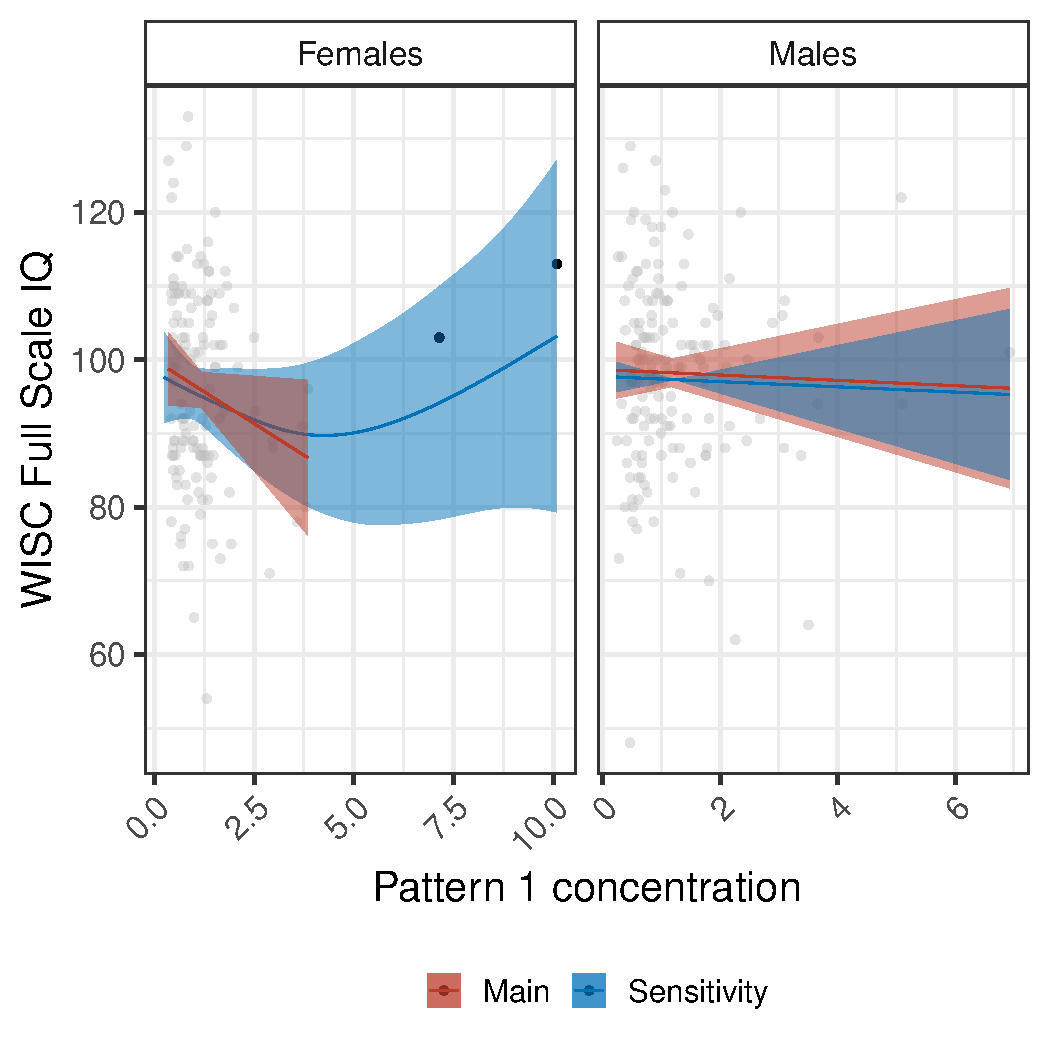
\includegraphics[scale = 0.85]{./figures/sense_plot.pdf}
\caption[Sensitivity analysis of associations in main analysis and full study sample]{Associations between phthalate + BPA pattern concentrations in pregnant women and children's full scale IQ at age 7 in the main analysis and sensitivity analysis. Models adjusted for maternal age, IQ, and education, prenatal alcohol consumption, marital status, HOME score, and material hardship. Shaded areas include 95\% confidence bands. Points represent measured data, with two influential outliers colored in black. Retaining these values in the data caused a deviation from linearity in females. Both extreme observations belonged to female children; their exclusion did not affect the relationship in males.}
\label{fig:fulldat}
\end{figure}
} % put supplemental numbering in curly braces


\chapter{Conclusion}\label{sec:conclusion}
\clearpage

This dissertation aimed to adapt pattern recognition methods employed in other fields (i.e., computer vision and machine learning) to environmental health data. We modified existing methods to remove the researcher from pattern number selection or specification, to retain the interpretability of a parts-based representation of data, and to explicitly account for uncertainty in identified patterns. We further incorporated this uncertainty in a hierarchical health model to understand the relationships between identified patterns of EDC exposure and child cognitive development. In this final chapter, we discuss our findings and their implications in three main sections: in Section~\ref{sec:summarize} we summarize our results and discuss their position within environmental mixtures research, in Section~\ref{sec:future} we discuss future research directions, and in Section~\ref{sec:ph} we conclude with the public health relevance and implications of our work.

\section{Findings \& environmental mixtures research}\label{sec:summarize}

\subsection{Dissertation findings}\label{sec:findings}
additions from this work

\subsection{Environmental mixtures}\label{sec:mixtures}
state of the science \\
examples, source apportionment

\subsection{Pattern recognition}\label{sec:patrec}
other methods \\
similar / different \\

\subsection{Bayesian methods}\label{sec:bayes}

\section{Future research directions}\label{sec:future}

\begin{itemize}
    \item tox studies
    \item coupling pattern recognition with other methods
    \item uncertainty propagation
    \item other mixtures
\end{itemize}

\section{Public Health relevance}\label{sec:ph}

\subsection{Research questions}\label{sec:question}
what questions should we be asking \\
research question should be informed by ultimate goal \\
what questions can we answer with this?

\subsection{Public Health implications}\label{sec:fin}

\begin{itemize}
    \item policy implications / informed interventions
    \item generalizability of patterns and of MN cohort
    \item biological mechanism not really with this method
\end{itemize}

\backmatter

% one bibliography for all chapters
\begin{SingleSpace}
    \linespread{1}
    \bibliographystyle{apalike}
    \bibliography{mix.bib}
\end{SingleSpace}

\end{document}